\documentclass[11pt]{article}

\usepackage[T1]{fontenc}
\usepackage[margin=1in]{geometry}
\usepackage{amsmath,amssymb,amsthm}
\usepackage{enumitem}
\usepackage{hyperref}
\usepackage{mathtools}
\usepackage{tikz}
\usepackage{framed}
\usepackage[hypcap=false]{caption}

\usetikzlibrary{arrows.meta}

\newcommand{\F}{\mathbb{F}}
\newcommand{\B}{\{0,1\}}
\newcommand{\Com}{\mathsf{Com}}
\newcommand{\Open}{\mathsf{Open}}
\newcommand{\Eval}{\mathsf{Eval}}
\newcommand{\Enc}{\mathsf{Enc}}
\newcommand{\Fold}{\mathsf{Fold}}
\newcommand{\MsgFold}{\mathsf{MsgFold}}
\newcommand{\CodeFold}{\mathsf{CodeFold}}
\newcommand{\RAA}{\mathsf{RAA}}
\newcommand{\PRAA}{\mathsf{PRAA}}
\newcommand{\MLE}{\mathsf{MLE}}
\newcommand{\PT}{\mathsf{PT}}
\newcommand{\Handle}{\mathsf{Handle}}
\newcommand{\bits}{\mathsf{bits}}
\newcommand{\Int}{\mathsf{int}}
\newcommand{\Idx}{\mathsf{idx}}
\newcommand{\RepView}{\mathsf{RepView}}
\newcommand{\ValueCheck}{\mathsf{ValueCheck}}
\newcommand{\PermCheck}{\mathsf{PermCheck}}
\newcommand{\AccCheck}{\mathsf{AccCheck}}
\newcommand{\Accumulate}{\mathsf{Accumulate}}
\newcommand{\Permute}{\mathsf{Permute}}
\newcommand{\SumReq}{\mathsf{SumReq}}
\newcommand{\MLEAuth}{\mathsf{MLEAuth}}
\newcommand{\Pad}{\mathsf{Pad}}
\newcommand{\prover}{\mathbb{P}}
\newcommand{\verifier}{\mathbb{V}}
\newcommand{\ip}[2]{\left\langle #1,#2 \right\rangle}

\newtheorem{definition}{Definition}
\newtheorem{lemma}{Lemma}
\newtheorem{theorem}{Theorem}
\newtheorem{remark}{Remark}

\newenvironment{protocolbox}[2]
  {\par\medskip\noindent\begin{minipage}{\textwidth}\begin{framed}\noindent\captionof{figure}{#1}\label{#2}\par\smallskip}
  {\end{framed}\end{minipage}\par\medskip}

\title{A First-Principles Theory of the Blaze/BaseFold Backend}
\author{A self-contained explainer for \texttt{cfri}}
\date{\today}

\begin{document}
\maketitle

\begin{abstract}
This paper explains the Blaze/BaseFold backend from first principles.  The goal
is not to specify byte formats or implementation APIs, but to explain the
mathematical object that the protocol proves and why its pieces fit together.
We start with finite fields, tensors, the multilinear extension (MLE), Merkle
commitments, linear codes, sumcheck, and BaseFold.  We then build the RAA
relation code, the Blaze interleaved commitment, the row-combining trick, the
evaluation-binding sumcheck, the RAA consistency relations, and the holographic
systematic backend that authenticates all terminal claims through one shared
fold spine.  No prior knowledge of tensor commitments, sumcheck protocols,
BaseFold, Blaze, or MLEs is assumed.
\end{abstract}

\tableofcontents

\section{A Gentle Map Of The Destination}

Blaze is a protocol for proving evaluations of large committed tensors while
reading only a small number of symbols.  The final construction uses several
pieces at once: finite-field arithmetic, multilinear extensions, commitments,
linear error-correcting codes, sumcheck, row compression, interleaving, RAA
encoding, and BaseFold-style proximity checks.

This paper builds those pieces bottom-up.  First we define the algebraic objects:
fields, tensors, multilinear extensions, commitments, codes, sumcheck, and
folding.  Then we explain Blaze's code-independent compression step: encode many
row slices, combine their committed row words into an openable folded tensor
$c_\star$, and bind $c_\star$ back to the committed matrix.  Only after that do we instantiate
the linear code with RAA and explain the correlated checks that make the proof
sound.

The one high-level idea to keep in mind is this: the protocol does not run code
checks and tensor-evaluation checks in isolation.  The opened positions,
folded terminal values, and multilinear claims must all refer to the same
committed objects.  Much of the backend exists to maintain that correlation.

\section{Finite Fields From First Principles}

A field is a set in which one can add, subtract, multiply, and divide by any
nonzero element, with the usual algebraic rules.  Familiar examples include the
rational numbers and real numbers.  Cryptographic proof systems usually use
finite fields: fields with only finitely many elements.

The target implementation uses a binary field with $2^{128}$ elements,
\[
  \F_{2^{128}}
  =
  \F_2[X]/(X^{128}+X^7+X^3+X+1).
\]
This means an element is a polynomial of degree at most $127$ with coefficients
in $\{0,1\}$, and multiplication is reduced modulo the irreducible polynomial
$X^{128}+X^7+X^3+X+1$.  Addition is coefficient-wise addition modulo two, which
is bitwise XOR in the usual machine representation.

For the theory, the exact field is less important than three properties:

\begin{enumerate}[label=\textbf{F\arabic*.}]
  \item We can perform field arithmetic exactly.
  \item The field is large enough that random field challenges make cheating
        unlikely.
  \item Linear equations and low-degree polynomial identities can be tested by
        evaluating them at random points.
\end{enumerate}

The protocol relies heavily on linearity.  If $A$ is a linear map, then
\[
  A(\alpha x+\beta y)=\alpha A(x)+\beta A(y).
\]
This simple equation is the reason Blaze can collapse $t$ committed row words
into one openable tensor $c_\star$ and ask the backend to prove one RAA
relation about it.

\section{Tensors, Flat Vectors, And Inner Products}

A tensor is a multi-dimensional array.  In this paper the most common tensor is
an order-$\ell$ tensor of shape $2\times\cdots\times2$, meaning it has one field
value for every Boolean address $b=(b_0,\ldots,b_{\ell-1})\in\B^\ell$.  We write
that entry as $x[b]$.

Formally, such a tensor is a function
\[
  x:\B^\ell\to\F.
\]
We write the vector space of all such tensors as
\[
  \F^{\B^\ell}.
\]
Thus saying $x\in\F^{\B^\ell}$ means exactly that $x$ assigns one field element
to each Boolean address in $\B^\ell$.

This tensor notation is the mathematical object.  Implementations eventually
serialize the same entries into a flat vector for memory, Merkle leaves, and
codeword coordinates:
\[
  x=(x[0],x[1],\ldots,x[N-1]).
\]
Here $N=2^\ell$.  The serialization is a deterministic address order for the
Boolean entries.  In this paper it is always the natural binary order.  For
\(0\le i<2^\ell\), write
\[
  \bits_\ell(i)\in\B^\ell
\]
for the length-\(\ell\) binary expansion of \(i\), with leading zeros included.
Then the \(i\)-th serialized entry is the tensor entry
\[
  x[\bits_\ell(i)].
\]
For an integer interval \([s,t]\subseteq[0,2^\ell-1]\), write
\[
  \bits_\ell([s,t])
  :=
  \{\bits_\ell(i):s\le i\le t\}\subseteq\B^\ell.
\]
This notation is only an implementation shorthand for a set of Boolean
addresses.  Protocol statements still use the binary address set.  For product
domains such as \(\B^a\times\B^b\), the natural layout is the lexicographic
binary layout induced by concatenation \((u,v)\mapsto u\Vert v\in\B^{a+b}\).
That order matters for implementors, because it tells them which memory
locations are paired in a fold or adjacent in an accumulator, but it is not the
algebraic object being folded.

The inner product of two tensors of the same shape is the sum of entrywise
products:
\[
  \ip{x}{y}=\sum_{b\in\B^\ell} x[b]y[b].
\]
After serializing both tensors with the same address order, this is implemented
as the usual inner product of two length-$N$ flat vectors:
\[
  \ip{x}{y}=\sum_{i=0}^{N-1} x[i]y[i].
\]
Many claims in this protocol reduce to inner products.  In particular, the
evaluation of a multilinear extension can be written as an inner product between
the original tensor and a tensor of public evaluation weights.  The protocol
uses both views constantly: the tensor view is the algebraic view for Boolean
addresses and MLEs, while the flat-vector view is the implementation view for
storage, commitments, and linear-algebra kernels.

\section{The Multilinear Extension}

In this paper, MLE means \emph{multilinear extension}, not maximum likelihood
estimation.  It is one of the central objects in modern polynomial-commitment
and sumcheck protocols.

\begin{definition}[Multilinear polynomial]
A polynomial $P(X_0,\ldots,X_{d-1})$ is multilinear if every variable has degree
at most one.  For example,
\[
  3+5X_0+7X_1+11X_0X_1
\]
is multilinear in $X_0,X_1$, but $X_0^2+X_1$ is not.
\end{definition}

\begin{definition}[Multilinear extension]
Let $f\in\F^{\B^d}$ be an order-$d$ tensor.  Its multilinear extension
$\MLE(f):\F^d\to\F$ is the unique multilinear polynomial
that agrees with $f$ on the Boolean hypercube:
\[
  \MLE(f)(b)=f(b)
  \qquad
  \text{for every }b\in\B^d.
\]
\end{definition}

The explicit formula is
\[
  \MLE(f)(z)
  =
  \sum_{b\in\B^d}
    f(b)\chi_b(z),
\]
where
\[
  \chi_b(z)
  =
  \prod_{h=0}^{d-1}
  \bigl((1-b_h)(1-z_h)+b_hz_h\bigr).
\]
The polynomial $\chi_b$ is an indicator polynomial.  It equals $1$ at Boolean
point $b$ and equals $0$ at every other Boolean point.

If an implementation receives the entries as a flat vector of length $2^d$, the
algebraic object is still a tensor $m\in\F^{\B^d}$ obtained by deserializing
those entries into Boolean addresses.  Then
\[
  \MLE(m)(z)
  =
  \sum_{b\in\B^d} m[b]\mu_z[b],
\]
where $\mu_z[b]=\chi_b(z)$ is the public evaluation weight for Boolean address
$b$.  Thus an MLE evaluation is an inner product:
\[
  \MLE(m)(z)=\ip{\mu_z}{m}.
\]

\subsection{A Two-Variable Example}

Suppose $m\in\F^{\B^2}$, with entries
$m[0,0]=m_{00}$, $m[0,1]=m_{01}$, $m[1,0]=m_{10}$, and
$m[1,1]=m_{11}$.  Its MLE is
\[
\begin{aligned}
  \MLE(m)(X_0,X_1)
  &=
  m_{00}(1-X_0)(1-X_1)
  + m_{01}(1-X_0)X_1\\
  &\quad
  + m_{10}X_0(1-X_1)
  + m_{11}X_0X_1.
\end{aligned}
\]
At $(0,0)$ this equals $m_{00}$; at $(0,1)$ it equals $m_{01}$; and so on.
At a non-Boolean point, it is an interpolation of the tensor entries.

\begin{figure}[h]
\centering
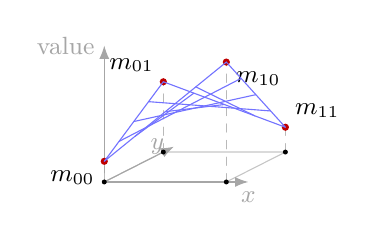
\begin{tikzpicture}[
  x={(1.55cm,0cm)},
  y={(0.75cm,0.38cm)},
  z={(0cm,1.05cm)},
  >=Latex,
  line cap=round,
  line join=round,
  font=\small
]
  \def\hzerozero{0.25}
  \def\honezero{1.45}
  \def\hzeroone{0.85}
  \def\honeone{0.30}

  \draw[gray!45] (0,0,0) -- (1,0,0) -- (1,1,0) -- (0,1,0) -- cycle;
  \draw[-Latex,gray!70] (0,0,0) -- (1.18,0,0) node[below] {$x$};
  \draw[-Latex,gray!70] (0,0,0) -- (0,1.18,0) node[left] {$y$};
  \draw[-Latex,gray!70] (0,0,0) -- (0,0,1.65) node[left] {value};

  \foreach \x/\y/\h in {
    0/0/\hzerozero,
    1/0/\honezero,
    0/1/\hzeroone,
    1/1/\honeone
  } {
    \draw[gray!55,dashed] (\x,\y,0) -- (\x,\y,\h);
    \fill[black] (\x,\y,0) circle (0.9pt);
    \fill[red!75!black] (\x,\y,\h) circle (1.3pt);
  }
  \node[below left] at (0,0,\hzerozero) {$m_{00}$};
  \node[below right] at (1,0,\honezero) {$m_{10}$};
  \node[above left] at (0,1,\hzeroone) {$m_{01}$};
  \node[above right] at (1,1,\honeone) {$m_{11}$};

  \foreach \x in {0,0.25,0.5,0.75,1} {
    \draw[blue!55]
      plot[variable=\y,domain=0:1,samples=25]
      ({\x},{\y},{(1-\x)*(1-\y)*\hzerozero + \x*(1-\y)*\honezero
        + (1-\x)*\y*\hzeroone + \x*\y*\honeone});
  }
  \foreach \y in {0,0.25,0.5,0.75,1} {
    \draw[blue!55]
      plot[variable=\x,domain=0:1,samples=25]
      ({\x},{\y},{(1-\x)*(1-\y)*\hzerozero + \x*(1-\y)*\honezero
        + (1-\x)*\y*\hzeroone + \x*\y*\honeone});
  }
\end{tikzpicture}
\caption{A two-variable multilinear extension as a bilinear interpolating surface.  The tensor $m$ gives values at Boolean corners; $\MLE(m)$ fills in the unique surface linear in each coordinate.}
\label{fig:two-variable-mle}
\end{figure}

\subsection{Folding Is MLE Evaluation One Variable At A Time}

Folding is most naturally expressed on the tensor itself.  Throughout this
paper, when we write a fold formula, we use the convention that the folded
coordinate is the last tensor coordinate.  More general coordinate folds are the
same operation after reordering coordinates.

Let $x\in\F^{\B^d}$.  For $a\in\B^{d-1}$ and $b\in\B$,
write $(a\mid b)\in\B^d$ for the concatenation of the length-$(d-1)$ address
$a$ and the final bit $b$.

For example, if $d=3$ and $a=(1,0)$, then
\[
  (a\mid 0)=(1,0,0),
  \qquad
  (a\mid 1)=(1,0,1).
\]
Folding the last coordinate at a field element $\lambda$ produces a tensor
$x^\star\in\F^{\B^{d-1}}$:
\[
  x^\star[a]
  =
  (1-\lambda)x[(a\mid 0)]
  +
  \lambda x[(a\mid 1)].
\]
This operation evaluates one MLE variable at $\lambda$ and removes that tensor
coordinate.  If we fold all coordinates, using one challenge for each coordinate
in the order those coordinates are removed, the final scalar is
\[
  \MLE(x)(\lambda_0,\ldots,\lambda_{d-1}).
\]

For implementors, the same fold becomes pairwise interpolation in the serialized
array.  If the chosen coordinate is laid out so that entries with that bit equal
$0$ occupy the first half and entries with that bit equal $1$ occupy the second
half, then the coordinate fold is implemented by
\[
  x'[i]=(1-\lambda)x[i]+\lambda x[i+L],
  \qquad 0\le i<L.
\]
That flat formula is a storage layout for the tensor fold, not the definition
of the fold itself.

\section{The Authenticated Opening Functionality}

The algebraic protocols below need authenticated oracle access.  A commitment
binds the prover to a logical tensor and later lets the verifier authenticate
selected entries at named addresses.  We will use this through a generic
functionality; a Merkle tree is one implementation, but not the only one we will
need.  The committed object carries its own natural address space.  If that
address space is \(\B^d\), the Merkle implementation uses the natural binary
leaf order
\[
  \bits_d(0),\bits_d(1),\ldots,\bits_d(2^d-1).
\]
If the address space is a product of binary domains, the leaf order is the
natural binary order after concatenating the address blocks.  Thus the
commitment API does not hide any indexing convention: the logical address space
is the layout.

\begin{protocolbox}{Functionality: $\mathcal{F}_{\mathrm{Commit}}$}{fig:func-commit}
For a committed tensor \(x\in\mathcal L^D\), the address set \(D\) and value
space \(\mathcal L\) are the natural ones carried by \(x\).

\smallskip
\noindent\(\underline{\mathcal{F}_{\mathrm{Commit}}.\Com(\prover:x,\ \verifier:\bot)\to R}\)

\smallskip
\begin{enumerate}[leftmargin=0.24in,label=\textbf{C\arabic*.},itemsep=0.08em,topsep=0.1em,parsep=0pt]
  \item \(\prover\to\mathcal F_{\mathrm{Commit}}\): \(x\in\mathcal L^D\).
  \item \(\mathcal F_{\mathrm{Commit}}\): choose a fresh handle \(R\) and store
        \(x\) under \(R\).  The address set \(D\) and value space
        \(\mathcal L\) are part of the tensor type of \(x\).
  \item \(\prover\to\verifier\): \(R\).
\end{enumerate}

\smallskip
\noindent\(\underline{\mathcal{F}_{\mathrm{Commit}}.\Open(\prover:R,\ \verifier:(R,a\in D))\to o\in\mathcal L\cup\{\bot\}}\)

\smallskip
\begin{enumerate}[leftmargin=0.24in,label=\textbf{O\arabic*.},itemsep=0.08em,topsep=0.1em,parsep=0pt]
  \item \(\prover\to\verifier\): opening data for \((R,a)\).
  \item \(\verifier\): return \(o=x[a]\) if the opening authenticates against
        \(R\); otherwise return \(\bot\).
\end{enumerate}
\end{protocolbox}

The commit call does not separately take \(D\) or \(\mathcal L\): these are the
natural address set and value space of the object being committed.  In the
codeword commitments below, $\mathcal{L}=\F$.  If
$\mathcal{F}_{\mathrm{Commit}}.\Open(R,a)\ne\bot$, its value is the unique
logical value $x[a]$ bound to $R$.  Equivalently, a verifier can check a claimed
value $v$ by opening $R$ at $a$ and checking that the returned value equals $v$.

In a real Merkle implementation, the handle $R$ is the Merkle root.  To compute
it for \(x\in\mathcal L^{\B^d}\), the prover serializes leaves as
\[
  x[\bits_d(0)],x[\bits_d(1)],\ldots,x[\bits_d(2^d-1)],
\]
hashes neighboring pairs, and keeps the final root.  To open address
\(a=\bits_d(i)\), the prover sends \(v=x[a]\) and the sibling hashes along the
path from the \(i\)-th leaf to the root.  The verifier recomputes the path and
checks that it ends at \(R\).

We will use several implementations of this same API.  The ordinary
implementation is Merkle: $\Pi_{\mathrm{merkleCommit}}.\Com(x)$
stores the logical tensor itself and opens coordinates by Merkle paths.  Blaze
also uses virtual handles: a virtual handle does not store one flat tensor
directly, but it still implements the same $\Com/\Open$ behavior.  We use two
virtual implementations.  The first, \(\Pi_{\mathrm{rowFoldCommit}}\), folds the
committed row-word matrix into the folded-tensor handle \(R_\star\).
The second, \(\Pi_{\mathrm{backendCommit}}\), extends \(R_\star\) with the
auxiliary RAA lanes and exposes the full backend message handle \(C_A\).

For example, if $R_c$ is a handle to a column tensor
$C\in(\F^{\B^\ell})^{\B^n}$ and $\rho\in\F^{\B^\ell}$, then a compressed
\(\Pi_{\mathrm{rowFoldCommit}}.\mathsf{Commit}(R_c,\rho)\) returns a handle
\(R_\star\) whose logical domain is \(\B^n\) and whose logical tensor is
\[
  c_\star[b]=\ip{\rho}{C[b]}.
\]
Opening $R_\star$ at $b$ opens the column $C[b]$ through $R_c$ and returns the
inner product with $\rho$.  The backend sees only the handle $R_\star$ and the
operation $\mathcal{F}_{\mathrm{Commit}}.\Open(R_\star,b)$.

The backend message handle is virtual in the same sense.  It is a handle over
the lane domain $\mathcal L\times\B^n$.  Opening lane \(0\) routes to
$R_\star$; opening the RAA lanes routes through the single residual-phase handle
\(C_{\mathrm{raa}}\).  BaseFold sees only this one backend handle, not the
machinery behind each lane.

We will also use a composite handle.  This is just public routing between
existing handles over disjoint coordinate sets; it is not a new cryptographic
assumption.

\begin{protocolbox}{Functionality: Composite Commitment}{fig:func-composite-commit}
\noindent Public parameters: disjoint address sets
\(E_1,\ldots,E_m\), local value spaces \(\mathcal L_i\), and component handles
\(R_i\), where \(R_i\) opens a tensor over address set \(E_i\).  The composite
domain is the disjoint union \(D=E_1\sqcup\cdots\sqcup E_m\).  The address sets
may be binary address sets, product sets, tagged sets, or any other disjoint
sets named by the protocol.

\smallskip
\noindent\(\underline{\mathsf{CompositeCommit}((R_1,E_1),\ldots,(R_m,E_m))\to R}\)

\smallskip
\begin{enumerate}[leftmargin=0.24in,label=\textbf{M\arabic*.},itemsep=0.08em,topsep=0.1em,parsep=0pt]
  \item \(\prover,\verifier\): return the handle \(R\) that stores the routing
        table \(((R_1,E_1),\ldots,(R_m,E_m))\).
\end{enumerate}

\smallskip
\noindent\(\underline{\mathsf{CompositeOpen}(R,a\in D)\to o\in\bigcup_i\mathcal L_i\cup\{\bot\}}\)

\smallskip
\begin{enumerate}[leftmargin=0.24in,label=\textbf{M\arabic*.},resume,itemsep=0.08em,topsep=0.1em,parsep=0pt]
  \item \(\prover,\verifier\): let \(i\) be the unique index with \(a\in E_i\).
  \item \(\prover,\verifier\): return
        \(o=\mathcal{F}_{\mathrm{Commit}}.\Open(R_i,a)\).
\end{enumerate}
\end{protocolbox}

For the systematic split used by BaseFold, the message addresses are
\(\mathcal L\times\B^k\).  The codeword addresses are
\(\mathcal L\times\B^n\).  The systematic address of
\((q,a)\in\mathcal L\times\B^k\) is \((q,0^{n-k}\Vert a)\).  Thus
\[
  D_{\mathrm{sys}}
  =
  \{(q,0^{n-k}\Vert a):q\in\mathcal L,\ a\in\B^k\},
  \qquad
  D_{\mathrm{ext}}
  =
  \mathcal L\times\bigl(\B^n\setminus\bits_n([0,2^k-1])\bigr).
\]
The composite handle is
\[
  \mathsf{CompositeCommit}
  ((C_A,D_{\mathrm{sys}}),(C_{\mathrm{ext}},D_{\mathrm{ext}})).
\]
Here \(C_A\) is viewed as a handle over \(D_{\mathrm{sys}}\): its value at
\((q,0^{n-k}\Vert a)\) is the message value \(A_q[a]\).  The composite handle
opens systematic codeword addresses through \(C_A\), and opens the remaining
codeword addresses through \(C_{\mathrm{ext}}\).

The functionality is binding at the logical-tensor level.  It is not an
algebraic commitment: it does not by itself prove that the logical tensor is a
codeword or that it satisfies any relation.  The algebraic proof comes from
random queries and low-degree/folding checks layered on top of these
authenticated openings.

\section{The Ideal Polynomial Commitment Functionality}

A polynomial commitment scheme, or PCS, is the object we ultimately want.  It
binds the prover to one polynomial before the verifier chooses evaluation
questions.  The clean ideal functionality is representation-free.

\begin{protocolbox}{Ideal Functionality: $\mathcal{F}_{\mathrm{PCS}}$}{fig:func-pcs}
Public parameter: number of variables \(d\).

\smallskip
\noindent\(\underline{\mathcal{F}_{\mathrm{PCS}}.\mathsf{Commit}(\prover:f,\ \verifier:\bot)\to C}\), for \(f:\F^d\to\F\).

\smallskip
\begin{enumerate}[leftmargin=0.24in,label=\textbf{P\arabic*.},itemsep=0.08em,topsep=0.1em,parsep=0pt]
  \item \(\prover\to\mathcal{F}_{\mathrm{PCS}}\): \(f\).
  \item \(\mathcal{F}_{\mathrm{PCS}}\): choose a fresh handle \(C\).
  \item \(\mathcal{F}_{\mathrm{PCS}}\): store \(f\) under \(C\).
  \item \(\mathcal{F}_{\mathrm{PCS}}\to\prover,\verifier\): \(C\).
\end{enumerate}

\smallskip
\noindent\(\underline{\mathcal{F}_{\mathrm{PCS}}.\mathsf{Evaluate}(\prover:\bot,\ \verifier:(C,z,v))\to b}\), for \(z\in\F^d\), \(v\in\F\), and \(b\in\{0,1\}\).

\smallskip
\begin{enumerate}[leftmargin=0.24in,label=\textbf{E\arabic*.},itemsep=0.08em,topsep=0.1em,parsep=0pt]
  \item \(\mathcal{F}_{\mathrm{PCS}}\): retrieve \(f\) stored under \(C\).
  \item \(\mathcal{F}_{\mathrm{PCS}}\): if \(f(z)=v\), set \(b\gets1\); otherwise set \(b\gets0\).
  \item \(\mathcal{F}_{\mathrm{PCS}}\to\verifier\): \(b\).
\end{enumerate}
\end{protocolbox}

The functionality in Figure~\ref{fig:func-pcs} deliberately commits to the
polynomial $f$, not to a particular array representation of $f$.  A concrete
protocol must choose such a representation.  In this paper, the tensor symbol
$y$ will mean whichever representation is being used at that point, and we will
say what it represents before using an evaluation formula.

Two representations are especially common.  If $y\in\F^{\B^d}$ stores Boolean
evaluations, then
\[
  y[b]=f(b)
  \qquad\text{and}\qquad
  f=\MLE(y).
\]
In that case
\[
  f(z)
  =
  \sum_{b\in\B^d} y[b]\chi_b(z),
\]
where
\[
  \chi_b(z)
  =
  \prod_{i=0}^{d-1}\bigl(b_i z_i+(1-b_i)(1-z_i)\bigr).
\]
If instead $y$ stores multilinear coefficients, then
\[
  f(X_0,\ldots,X_{d-1})
  =
  \sum_{b\in\B^d} y[b]\prod_{i=0}^{d-1}X_i^{b_i}.
\]
In that case
\[
  f(z)
  =
  \sum_{b\in\B^d} y[b]\prod_{i=0}^{d-1}z_i^{b_i}.
\]
These are different tensors related by a linear change of basis.  The protocol
goal $f(z)=v$ is the same, but the public weights in the sum are different.
We should therefore never infer $f=\MLE(y)$ unless $y$ has just been declared to
be the Boolean-evaluation tensor.

The simplest concrete implementation of Figure~\ref{fig:func-pcs} is to reveal
the entire representation tensor to the verifier.  Figure~\ref{fig:protocol-trivial-pcs}
is useful as a baseline: it is correct, but it gives up succinctness completely.

\begin{protocolbox}{Protocol: Trivial PCS}{fig:protocol-trivial-pcs}
\noindent\(\underline{\mathsf{TrivialPCS.Commit}(\prover:y,\ \verifier:\bot)\to C}\)

\smallskip
\begin{enumerate}[leftmargin=0.24in,label=\textbf{T\arabic*.},itemsep=0.08em,topsep=0.1em,parsep=0pt]
  \item \(\prover\to\verifier\): \(y\).
  \item \(\verifier\): \(C\gets y\).
  \item \(\verifier\): return \(C\).
\end{enumerate}

\smallskip
\noindent\(\underline{\mathsf{TrivialPCS.Evaluate}(\prover:y,\ \verifier:(C,z,v))\to\{0,1\}}\)

\smallskip
\begin{enumerate}[leftmargin=0.24in,label=\textbf{U\arabic*.},itemsep=0.08em,topsep=0.1em,parsep=0pt]
  \item \(\verifier\): compute \(u=f_C(z)\) from the stored tensor \(C\).
  \item \(\verifier\): if \(u\ne v\), return reject.
  \item \(\verifier\): return accept.
\end{enumerate}
\end{protocolbox}

The protocol in Figure~\ref{fig:protocol-trivial-pcs} is correct.  It is also
exactly what we are trying to avoid.  It leaks the whole polynomial
representation and makes the verifier store or scan $2^d$ field elements.  For
the discussion here, privacy is not the central problem; efficiency and binding
are.  Later versions of polynomial commitments may also hide $f$, but the
Blaze/BaseFold backend is already interesting before adding hiding.

\section{Sumcheck As Claim Randomization}

Our target is the PCS functionality from Figure~\ref{fig:func-pcs}.  After the
prover is bound to a multilinear polynomial $f:\F^d\to\F$, the verifier should
be able to check evaluation claims of the form
\[
  (C,z,v)\longmapsto 1
  \qquad\text{iff}\qquad
  f(z)=v,
\]
where $C$ is the commitment handle.  Sumcheck does not implement this
functionality by itself.  Instead, it transforms one evaluation claim about the
committed polynomial into another evaluation claim about the same committed
polynomial:
\[
  (C,z,v)\quad\rightsquigarrow\quad(C,r,u).
\]
This does not remove the need to verify the new claim $(C,r,u)$.  From a pure
API viewpoint, it is a PCS claim $(C,z,v)$ transformed into another PCS claim
$(C,r,u)$.  The improvement is in the distribution of the point.  The original
point $z$ may be known before the prover commits; the new point $r$ in
$(C,r,u)$ is sampled by the verifier after the prover is bound to the
commitment and to the sumcheck messages.  As protocol designers, that
randomization is valuable.

The first step is to express the claim $f(z)=v$ as a claim about the Boolean
cube.  A multilinear polynomial is determined by its values on $\B^d$.  For
$b\in\B^d$, define the Boolean interpolation weight
\[
  \chi_b(z)
  =
  \prod_{i=0}^{d-1}\bigl(b_i z_i+(1-b_i)(1-z_i)\bigr).
\]
These weights project the arbitrary point $z$ back onto the Boolean cube:
\[
  f(z)
  =
  \sum_{b\in\B^d} f(b)\chi_b(z).
\]
This identity is not an optimization.  It only rewrites the arbitrary-point
claim as a weighted Boolean-cube sum.

For fixed $z$, it is convenient to put the weights into a polynomial whose
variable is the Boolean-cube point being summed over:
\[
  \chi_z(Y)
  =
  \prod_{i=0}^{d-1}\bigl((1-Y_i)(1-z_i)+Y_i z_i\bigr).
\]
At a Boolean point $b$, this gives $\chi_z(b)=\chi_b(z)$.  Therefore, if
\[
  H(Y)=f(Y)\chi_z(Y),
\]
then the PCS claim is equivalent to
\[
  f(z)=v
  \qquad\Longleftrightarrow\qquad
  \sum_{b\in\B^d}H(b)=v.
\]
Even though $f$ and $\chi_z$ are multilinear, their product $H$ is generally
not multilinear: a variable can have degree two.  This is fine.  Sumcheck does
not require multilinearity.  It requires a known bound on the individual degree
of $H$ in each variable, because that bound controls the degree of each
univariate round polynomial.
The verifier could check this by reading all Boolean values of $f$, but that is
the trivial PCS of Figure~\ref{fig:protocol-trivial-pcs} again.  Sumcheck keeps
the Boolean-sum meaning while replacing the endpoint by a random point.

\paragraph{Evaluation and coefficient views.}
The discussion above used the Boolean values
\[
  b\longmapsto f(b),
  \qquad b\in\B^d,
\]
because that is the cleanest way to see why the interpolation weights
$\chi_b(z)$ recover $f(z)$.  This is an \emph{evaluation view}: the tensor is
the table of values of $f$ on the Boolean cube.

The same multilinear polynomial can also be represented by a coefficient tensor
$y\in\F^{\B^d}$:
\[
  f(X_0,\ldots,X_{d-1})
  =
  \sum_{b\in\B^d} y[b]\prod_{i=0}^{d-1}X_i^{b_i}.
\]
This is a different basis for the same object, not a different polynomial.  For
example, when $d=1$,
\[
  f(X)=y[0]+y[1]X,
  \qquad
  (f(0),f(1))=(y[0],y[0]+y[1]).
\]
Either representation determines the other by a linear change of basis.

Sumcheck is easiest to motivate in the evaluation view because it starts with a
Boolean-cube sum.  The concrete BaseFold construction is easiest to fold in the
coefficient view.  For an $(i+1)$-variate multilinear polynomial, splitting the
coefficient tensor along the last Boolean coordinate writes
\[
  f(X_0,\ldots,X_i)
  =
  f_L(X_0,\ldots,X_{i-1})
  +
  X_i f_R(X_0,\ldots,X_{i-1}),
\]
and a challenge $\theta\in\F$ specializes that variable:
\[
  f(X_0,\ldots,X_{i-1},\theta)
  =
  f_L(X_0,\ldots,X_{i-1})
  +
  \theta f_R(X_0,\ldots,X_{i-1}).
\]
This is the coefficient-side version of a fold.  Later, when BaseFold commits to
a coefficient tensor, sumcheck is still talking about the same polynomial
function $f$; only the committed representation has changed.

\subsection{The Two-Variable Case}

Take $d=2$.  The verifier wants to check
\[
  H(0,0)+H(1,0)+H(0,1)+H(1,1)=v.
\]
The prover first sends a univariate polynomial
\[
  g_1(X)=H(0,X)+H(1,X).
\]
The verifier can check the claimed total without evaluating $H$:
\[
  g_1(0)+g_1(1)=v.
\]
If this passes, the verifier samples $r_1\leftarrow\F$, sends it to the prover,
and changes the claim to
\[
  H(0,r_1)+H(1,r_1)=g_1(r_1).
\]
One Boolean coordinate has disappeared.  The prover then sends
\[
  g_0(X)=H(X,r_1).
\]
The verifier checks
\[
  g_0(0)+g_0(1)=g_1(r_1),
\]
samples $r_0\leftarrow\F$, sends it to the prover, and changes the claim to
\[
  H(r_0,r_1)=g_0(r_0).
\]
Now there is no Boolean sum left.  Since $H(Y)=f(Y)\chi_z(Y)$, the last claim is
\[
  f(r_0,r_1)\chi_z(r_0,r_1)=g_0(r_0).
\]
The verifier can compute $\chi_z(r_0,r_1)$ locally.  It only needs one
remaining value of the committed polynomial $f$ at the random point
$(r_0,r_1)$.

The order matters.  The prover sends each $g_i$ before seeing the corresponding
random challenge $r_i$.  A false polynomial identity can agree at a random
field point only with small probability, bounded by its degree over $|\F|$.

\begin{protocolbox}{Protocol: Sumcheck Randomizes A PCS Evaluation Claim}{fig:protocol-sumcheck-randomizes-pcs}
\noindent Public input: \(C\), \(z\in\F^d\), \(v\in\F\).

\smallskip
\begin{enumerate}[leftmargin=0.24in,label=\textbf{S\arabic*.},itemsep=0.08em,topsep=0.1em,parsep=0pt]
  \item \(\verifier\): \(s_d\gets v\).
  \item For \(i=d-1,d-2,\ldots,0\):
        \begin{enumerate}[leftmargin=0.28in,label=\textbf{S\arabic*.\alph*.},itemsep=0.05em,topsep=0.05em,parsep=0pt]
          \item \(\prover\to\verifier\): \(g_i\in\F[X]\).
          \item \(\verifier\): if \(\deg(g_i)>2\), return reject.
          \item \(\verifier\): if \(g_i(0)+g_i(1)\ne s_{i+1}\), return reject.
          \item \(\verifier\): \(r_i\leftarrow\F\).
          \item \(\verifier\to\prover\): \(r_i\).
          \item \(\verifier\): \(s_i\gets g_i(r_i)\).
        \end{enumerate}
  \item \(\verifier\): \(r\gets(r_0,\ldots,r_{d-1})\).
  \item \(\verifier\): if \(\chi_z(r)=0\), return reject.
  \item \(\verifier\): \(u\gets s_0/\chi_z(r)\).
  \item \(\verifier\): \(b\gets\mathcal{F}_{\mathrm{PCS}}.\mathsf{Evaluate}(C,r,u)\).
  \item \(\verifier\): if \(b=0\), return reject.
  \item \(\verifier\): return \((1,C,r,u)\).
\end{enumerate}
\end{protocolbox}

The protocol in Figure~\ref{fig:protocol-sumcheck-randomizes-pcs} is
deliberately circular if the endpoint is the ideal PCS functionality from
Figure~\ref{fig:func-pcs}: we have transformed one PCS evaluation into another
PCS evaluation.  The reason to keep the transformation is that the new point
$r$ is verifier-random and transcript-bound.  BaseFold removes the circularity
by implementing this random endpoint from a commitment to an encoded oracle.  In
short, sumcheck randomizes the polynomial claim; BaseFold folds the
committed codeword along the same challenges.

\subsection{Inner-Product Sumcheck}

The same randomization idea also explains the inner-product checks used later by
Blaze.  Let
\[
  w,x\in\F^{\B^\ell}.
\]
For this subsection, both tensors are Boolean-evaluation tensors.  The verifier
knows $w$ and can compute with all of it.  The prover is bound to $x$ by some
commitment handle $C_x$, but the verifier should not have to read all of $x$.
The claim is
\[
  \sum_{b\in\B^\ell} w[b]x[b]=S.
\]
The objective is to move this full inner product to one claim about the
committed tensor $x$ at a verifier-random point.

Define the polynomial
\[
  H(Y)=\MLE(w)(Y)\MLE(x)(Y).
\]
On Boolean inputs, $H(b)=w[b]x[b]$.  Therefore the inner-product claim is
exactly the Boolean-sum claim
\[
  \sum_{b\in\B^\ell}H(b)=S.
\]
This $H$ is not generally multilinear, because it is a product of two
multilinear polynomials.  Its individual degree is at most two, and that is the
degree bound sumcheck needs.  Therefore the round polynomials are degree two.

Trace one round.  Suppose the active tensors are still indexed by $\B^d$ and
the current claim is their inner product:
\[
  \sum_{a\in\B^d} w[a]x[a]=s_d.
\]
To eliminate the last coordinate, write each address as $(a\mid b)$ with
$a\in\B^{d-1}$ and $b\in\B$.  For each $a\in\B^{d-1}$ define the two line
interpolants
\[
  w_a(X)=(1-X)w[(a\mid0)]+Xw[(a\mid1)],
\]
\[
  x_a(X)=(1-X)x[(a\mid0)]+Xx[(a\mid1)].
\]
The honest round polynomial is
\[
  p(X)=\sum_{a\in\B^{d-1}}w_a(X)x_a(X).
\]
This polynomial has a clear job:
\[
  p(0)+p(1)=s_d.
\]
After checking this equation, the verifier samples $r_{d-1}\leftarrow\F$, sends
it to the prover, and
the new claim becomes
\[
  \sum_{a\in\B^{d-1}} w_a(r_{d-1})x_a(r_{d-1})=s_{d-1},
  \qquad s_{d-1}=p(r_{d-1}).
\]
So one round folds both tensors by the same verifier challenge and replaces the
old inner product by a smaller inner product.

The verifier can perform the fold of $w$ locally, because $w$ is public.  It
cannot locally fold every entry of $x$, because $x$ is committed.  That is the
point of the randomization: after $\ell$ rounds, the verifier has folded $w$
down to the public scalar $\MLE(w)(r)$, and the sumcheck transcript has
produced a random point $r=(r_0,\ldots,r_{\ell-1})$ and a final scalar $s_0$.
Assuming $\MLE(w)(r)\ne0$ in this simplified presentation, the verifier sets
\[
  u=s_0/\MLE(w)(r).
\]
Thus the input inner-product claim has been transformed into the ordinary
committed-evaluation claim
\[
  (C_x,r,u).
\]
Here $(C_x,r,u)$ means that the tensor bound to $C_x$ should satisfy
$\MLE(x)(r)=u$.  This output claim is useful because it asks for one random
evaluation of the committed tensor $x$, not for all of $x$.  BaseFold is the
mechanism that later binds that value $u$ to the committed encoding of $x$ with
only a few openings.

\section{BaseFold From First Principles}

BaseFold combines two ingredients.  We first separate them so the role of each
one is clear.  The first is an IOP of proximity, or IOPP: it checks that an
oracle word is close to a codeword.  The second is the sumcheck protocol in
Figure~\ref{fig:protocol-sumcheck-randomizes-pcs}: it reduces $f(z)=v$ to a
random evaluation claim.  A polynomial commitment scheme appears only when
these two protocols are run together with the same challenges.

The central design question is simple.  Sumcheck wants to fold the message
representation: split the current message as $m=(m_L\mid m_R)$ and replace it
by $m_L+\alpha m_R$ for a verifier challenge $\alpha$.  But the verifier does
not have the raw message.  It has a commitment to an encoded oracle
$\pi=\Enc(m)$.  BaseFold is the answer to the question:
\[
  \text{can we fold the committed encoding as if we had folded the message?}
\]
The code is built so that the answer is yes.

\subsection{The IOPP Functionality}

Fix a public linear code $C\subseteq\F^N$.

\begin{protocolbox}{Ideal Functionality: $\mathcal{F}_{\mathrm{IOPP}}^C$}{fig:func-iopp}
\noindent Public parameters: code \(C\subseteq\F^N\), distance threshold
\(\delta\in[0,1]\).

\smallskip
\noindent\(\underline{\mathcal{F}_{\mathrm{IOPP}}^C.\mathsf{Submit}(\prover:\pi,\ \verifier:\bot)\to I}\)

\smallskip
\begin{enumerate}[leftmargin=0.24in,label=\textbf{I\arabic*.},itemsep=0.08em,topsep=0.1em,parsep=0pt]
  \item \(\prover\to\mathcal{F}_{\mathrm{IOPP}}^C\): \(\pi\in\F^N\).
  \item \(\mathcal{F}_{\mathrm{IOPP}}^C\): choose a fresh handle \(I\).
  \item \(\mathcal{F}_{\mathrm{IOPP}}^C\): store \(\pi\) under \(I\).
  \item \(\mathcal{F}_{\mathrm{IOPP}}^C\to\prover,\verifier\): \(I\).
\end{enumerate}

\smallskip
\noindent\(\underline{\mathcal{F}_{\mathrm{IOPP}}^C.\mathsf{Check}(\prover:\bot,\ \verifier:I)\to\{0,1\}}\)

\smallskip
\begin{enumerate}[leftmargin=0.24in,label=\textbf{J\arabic*.},itemsep=0.08em,topsep=0.1em,parsep=0pt]
  \item \(\mathcal{F}_{\mathrm{IOPP}}^C\): retrieve \(\pi\) stored under \(I\).
  \item \(\mathcal{F}_{\mathrm{IOPP}}^C\): \(\Delta_\pi\gets\min_{c\in C}\Delta(\pi,c)\).
  \item \(\mathcal{F}_{\mathrm{IOPP}}^C\): if \(\Delta_\pi\le\delta\), set \(b\gets1\); otherwise set \(b\gets0\).
  \item \(\mathcal{F}_{\mathrm{IOPP}}^C\to\verifier\): \(b\).
\end{enumerate}
\end{protocolbox}

The functionality in Figure~\ref{fig:func-iopp} is useful, but it is not a
PCS.  It says that the submitted word is close to \emph{some} valid codeword.
It does not say which polynomial was encoded, and it does not by itself prove
$f(z)=v$.  The PCS will use this proximity statement as one component.

\subsection{Concrete Foldable Codes}

Now specialize to the concrete foldable-code structure used by the BaseFold
paper.  For $i=0,\ldots,d$, let $C_i$ be a linear code with message tensor
domain $\B^{k_i}$ and codeword tensor domain $\B^{n_i}$.  The actual message
length is $K_i=2^{k_i}$, and the actual codeword length is $N_i=2^{n_i}$.
At each fold level one Boolean coordinate is removed, so
\[
  k_{i+1}=k_i+1,
  \qquad
  n_{i+1}=n_i+1.
\]
Let
\[
  \Enc_i:\F^{\B^{k_i}}\to\F^{\B^{n_i}}
\]
be its encoder.  Equivalently, with row-vector convention,
\[
  \Enc_i(m)=mG_i,
\]
where $G_i$ is the public generator matrix whose columns are indexed by
$\B^{n_i}$.

The code family is foldable because the next generator matrix is built from the
previous one using a public random diagonal matrix $T_i$ whose rows and columns
are indexed by $\B^{n_i}$.  Diagonal means that
\[
  T_i[a,a']=0
  \qquad\text{whenever } a\ne a'.
\]
In the concrete random foldable code, the diagonal entries
\[
  \{T_i[a,a]\}_{a\in\B^{n_i}}
\]
are sampled independently and uniformly from $\F$, then fixed as part of the
public code description:
\[
  G_{i+1}
  =
  \begin{bmatrix}
    G_i & G_i \\
    G_iT_i & G_i(T_i+I_i)
  \end{bmatrix}.
\]
Here $I_i$ is the identity matrix on $\F^{\B^{n_i}}$.
The two block columns are indexed by $(a,0)$ and $(a,1)$ for
$a\in\B^{n_i}$.  The diagonal entries of $T_i$ are part of the code
description.  Write
\[
  t_{i,a}=T_i[a,a]\in\F.
\]
Then the two interpolation points for coordinate $a$ are $t_{i,a}$ and
$t_{i,a}+1$.  These points are not chosen by the prover and are not verifier
challenges; they are fixed by the concrete random foldable code.

Split a message $m\in\F^{\B^{k_{i+1}}}$ as
\[
  m=(m_L\mid m_R),
  \qquad m_L,m_R\in\F^{\B^{k_i}}.
\]
If $\pi_{i+1}=\Enc_{i+1}(m)$, then for every $a\in\B^{n_i}$,
\[
  \pi_{i+1}[a,0]
  =
  \Enc_i(m_L)[a]+t_{i,a}\Enc_i(m_R)[a],
\]
\[
  \pi_{i+1}[a,1]
  =
  \Enc_i(m_L)[a]+(t_{i,a}+1)\Enc_i(m_R)[a].
\]
Thus these two symbols are evaluations of the same line
\[
  L_a(X)=\Enc_i(m_L)[a]+X\Enc_i(m_R)[a]
\]
at the two public code points $t_{i,a}$ and $t_{i,a}+1$.  If the verifier
later samples a challenge $\alpha_i\in\F$, evaluating the same line at
$\alpha_i$ gives
\[
  L_a(\alpha_i)
  =
  \Enc_i(m_L+\alpha_i m_R)[a].
\]
This is the concrete BaseFold fold.  It is a local interpolation rule on
codeword symbols, and its correctness comes from the displayed generator-matrix
decomposition.

Now we can name the two sides of the same operation.  The message fold is
\[
  \MsgFold_{\alpha_i}(m)=m_L+\alpha_i m_R\in\F^{\B^{k_i}}.
\]
The codeword fold is the local interpolation rule
\[
  \CodeFold_{\alpha_i}(\pi_{i+1})[a]=L_a(\alpha_i),
  \qquad a\in\B^{n_i},
\]
where $L_a$ is reconstructed from the two codeword symbols at the
code-specified points $t_{i,a}$ and $t_{i,a}+1$.  Foldability is the
commuting statement
\[
  \CodeFold_{\alpha_i}(\Enc_{i+1}(m))
  =
  \Enc_i(\MsgFold_{\alpha_i}(m)).
\]
This equation is the intuition that the protocol relies on: sumcheck asks for
the left-to-right message fold, while the verifier can only test the
top-to-bottom codeword fold through committed oracle openings.

\subsection{Minimum Distance And Johnson Radius}

The proof needs a way to talk about how close words can be to codewords, and
how close different codewords can be to each other.  The first tool is minimum
distance.  Half the minimum distance is the uniqueness radius: inside that
radius, a received word can be close to at most one codeword.  That is useful,
but it is not the whole story.  Just outside the uniqueness radius, there may be
more than one nearby codeword.  The proof also needs to know that there are not
too many of them.  Johnson's bound is the standard tool for controlling that
nearby list.

Let $C\subseteq\F^{\B^n}$ be a code.  For words $x,c\in\F^{\B^n}$, write
\[
  \Delta(x,c)
  =
  \frac{|\{a\in\B^n:x[a]\ne c[a]\}|}{2^n}
\]
for ordinary relative Hamming distance.  The relative minimum distance of $C$
is
\[
  \Delta_C
  =
  \min_{\substack{c,c'\in C\\ c\ne c'}}\Delta(c,c').
\]
Thus two distinct codewords disagree on at least a $\Delta_C$ fraction of
coordinates.

\paragraph{Random foldable codes have good minimum distance.}
For BaseFold's random foldable code (RFC), the minimum distance is not assumed by
magic; it is proved from the random diagonal matrices.  Let
$N_i=2^{n_i}$ be the actual codeword length at layer $i$.  The BaseFold
minimum-distance theorem says, in this paper's notation, that the random choice
of the foldable code gives an explicit lower bound
\[
  \Delta_{C_d}\ge \rho_{\mathrm{RFC}}
\]
except with small probability over the sampled diagonal matrices.  The quantity
$\rho_{\mathrm{RFC}}\in[0,1]$ is computed from the code parameters
$(k_0,d,c,|\F|)$; Appendix C of BaseFold gives the recurrence, and the theorem's
failure probability is, for example, on the order of $d\cdot 2^{-\lambda}$ for
security parameter $\lambda$.

The proof style is important.  Because the code is linear, the minimum distance
is the minimum Hamming weight of a nonzero codeword.  So the proof studies zeros:
how many coordinates of $\Enc_i(m)$ can vanish for a nonzero message $m$?
Inductively assume that level $i$ has few zeros for every nonzero message.  At
the next level, split $m=(m_L\mid m_R)$ and write the two previous-layer
encodings as
\[
  A=\Enc_i(m_L),
  \qquad
  B=\Enc_i(m_R).
\]
For each previous-layer coordinate $a\in\B^{n_i}$, the next codeword contains
two line evaluations whose slope is controlled by the random diagonal entry
$t_{i,a}$.  If $A[a]$ and $B[a]$ are not both zero, then the event that one of
those new symbols vanishes is essentially one linear equation in the random
field element $t_{i,a}$, hence has probability about $1/|\F|$.

A naive proof would now union bound over all nonzero messages, but that loses too
much: there are too many messages.  BaseFold's proof refines the union bound by
partitioning messages according to the common zero set
\[
  S=\{a:A[a]=0\text{ and }B[a]=0\}.
\]
Large sets $S$ are dangerous because those coordinates are automatically zero in
both halves, but rank-nullity says there are few messages that can have a large
common zero set.  Small sets $S$ allow many messages, but then many independent
random diagonal entries would need to hit unlucky roots.  The proof balances
these two effects: count messages by the size of $S$, apply a binomial-style
tail bound for the fresh random diagonal entries, and union bound over all
possible $S$.  That is how the random foldable code gets a concrete lower bound
on $\Delta_{C_d}$.

\paragraph{Minimum distance gives unique decoding below half distance.}
If a word $v\in\F^{\B^n}$ satisfies
\[
  \Delta(v,c)<\Delta_C/2,
  \qquad
  \Delta(v,c')<\Delta_C/2
\]
for two codewords $c,c'\in C$, then the triangle inequality gives
\[
  \Delta(c,c')
  \le
  \Delta(c,v)+\Delta(v,c')
  <
  \Delta_C.
\]
This contradicts the definition of $\Delta_C$ unless $c=c'$.  So inside radius
$\Delta_C/2$, there is at most one nearby codeword.  This is the basic
minimum-distance argument.

\paragraph{Johnson controls lists beyond half distance.}
Unique decoding says there is at most one nearby codeword below
$\Delta_C/2$.  List decoding asks a softer question beyond that radius: even if
there are several nearby codewords, can we bound how many there are?  Johnson's
bound gives such a radius using only the minimum distance of the code.

For a slack parameter $\gamma\in(0,1]$, define the Johnson-radius function
\[
  J_\gamma(\lambda)
  =
  1-\sqrt{1-\lambda(1-\gamma)}
  \qquad\text{for }\lambda\in[0,1].
\]
This is a slightly shrunken version of the usual Johnson radius
$1-\sqrt{1-\lambda}$.  The shrinkage gives the proof room for strict
inequalities and union bounds.

The proof intuition is a counting tension.  If many codewords are all within
relative distance $\rho$ of the same received word $v$, then each of them agrees
with $v$ on about a $1-\rho$ fraction of coordinates.  Averaging over pairs of
nearby codewords, many of those agreements must occur on the same coordinates,
so the nearby codewords agree with each other too often.  But distinct codewords
are required to disagree on at least a $\Delta_C$ fraction of coordinates.
Solving this tension gives a controlled list size as long as
$\rho$ is below the Johnson radius.

BaseFold uses this through the following one-step no-free-repair lemma.  Assume
the code minimum distances are monotone in the BaseFold direction, so the
top-layer minimum distance $\Delta_{C_d}$ is a valid lower bound for the layers
below.
Set
\[
  R_{\mathrm{BF}}
  =
  J_\gamma(J_\gamma(\Delta_{C_d})).
\]

\begin{lemma}[One-step no-free-repair lemma]
\label{lem:one-step-no-free-repair}
For any layer $i=0,\ldots,d-1$, any word
$v\in\F^{\B^{n_{i+1}}}$, and any $\eta\le R_{\mathrm{BF}}$, if
\[
  \Delta^*(v,C_{i+1})>\eta,
\]
then
\[
  \Pr_{\alpha_i\leftarrow\F}
  \left[
    \Delta(\CodeFold_{\alpha_i}(v),C_i)
    \le
    \eta-\gamma
  \right]
  \le
  \frac{2}{\gamma^3|\F|}.
\]
Here $\Delta^*$ is the paired/coset distance used by BaseFold: a parent pair is
counted as bad if either of its two entries disagrees with the candidate
codeword.
\end{lemma}

The proof idea matches the foldable-code structure above.  Any parent word
$v$ can be uniquely written as two point evaluations of a coordinatewise line,
so the possible folds $\CodeFold_{\alpha_i}(v)$ trace the affine family
$u+\alpha_i u'$.  If too many challenges $\alpha_i$ made this fold close to
some child codeword of $C_i$, Johnson/list decoding would force those nearby
child codewords to share enough structure to identify two codewords
$w,w'\in C_i$ agreeing with $u,u'$ on many coordinates.  Foldability then
combines $w$ and $w'$ into a parent codeword in $C_{i+1}$ that is close to
$v$ in paired/coset distance, contradicting
$\Delta^*(v,C_{i+1})>\eta$.  This is the formal reason adaptive free repairs
are rare.

\subsection{BaseFold IOPP}

Recall that an IOPP is an interactive oracle proof of proximity.  Its job is
not to prove an evaluation claim such as $f(z)=v$.  Its job is to convince the
verifier that a committed oracle is close to some codeword of a specified code.
BaseFold does this by asking the prover to commit to folded oracle layers and
then auditing a small number of local fold relations between adjacent layers.

First read the protocol in the honest direction.  Fix a number of fold layers
$d\in\mathbb{N}$.  The public objects are the field $\F$, the Boolean coordinate
alphabet $\B$, the log message and codeword dimensions
$k_i,n_i\in\mathbb{N}$ for $i=0,\ldots,d$, with
$k_{i+1}=k_i+1$ and $n_{i+1}=n_i+1$, the encoders
\[
  \Enc_i:\F^{\B^{k_i}}\to\F^{\B^{n_i}},
  \qquad
  C_i=\Enc_i(\F^{\B^{k_i}}),
\]
the code-specified interpolation points $t_{i,a}\in\F$ for
$i=0,\ldots,d-1$ and $a\in\B^{n_i}$, and a query count
$Q_{\mathrm{BF}}\in\mathbb{N}$.  The IOPP input oracle is a committed tensor
$\pi_d\in\F^{\B^{n_d}}$.  In an honest execution, the prover's private input is
a message tensor $m_d\in\F^{\B^{k_d}}$, and the committed top oracle is
\[
  \pi_d=\Enc_d(m_d)\in\F^{\B^{n_d}}.
\]
For each layer $i=d-1,\ldots,0$, the verifier samples a fresh challenge
$\alpha_i\leftarrow\F$, sends it to the prover, and then the prover commits to
the next child oracle.  In
the concrete coefficient-style BaseFold convention of the previous subsection,
the honest prover splits $m_{i+1}=(m_L\mid m_R)$ with
$m_L,m_R\in\F^{\B^{k_i}}$ and sets
\[
  m_i=\MsgFold_{\alpha_i}(m_{i+1})=m_L+\alpha_i m_R.
\]
The honest child oracle is then
\[
  \pi_i=\Enc_i(m_i).
\]
Equivalently, and this is the form the verifier can test, for every
$a\in\B^{n_i}$ the value $\pi_i[a]$ is obtained by interpolating the line through
the two parent symbols
\[
  (t_{i,a},\pi_{i+1}[a,0])
  \qquad\text{and}\qquad
  (t_{i,a}+1,\pi_{i+1}[a,1])
\]
and evaluating that line at $\alpha_i$.  Thus the honest invariant is
\[
  \pi_i=\Enc_i(m_i),
\]
where $m_i$ is the folded message determined by the challenges already sampled.
The verifier cannot check this invariant everywhere, so
Figure~\ref{fig:protocol-basefold-iopp} authenticates the committed oracles and
then checks a few complete parent-child paths.

\begin{protocolbox}{Protocol: BaseFold IOPP}{fig:protocol-basefold-iopp}
\label{fig:protocol-basefold-iopp-query}
\noindent Public parameters: \(d,Q_{\mathrm{BF}}\in\mathbb{N}\), codes
\(\mathcal{C}_i\subseteq\F^{\B^{n_i}}\), interpolation points
\(t_{i,a}\in\F\) for \(i=0,\ldots,d-1\) and \(a\in\B^{n_i}\).

\smallskip
\begin{enumerate}[leftmargin=0.24in,label=\textbf{P\arabic*.},itemsep=0.08em,topsep=0.1em,parsep=0pt]
  \item \(\prover\): \(R_d\gets\mathcal{F}_{\mathrm{Commit}}.\Com(\pi_d)\).
  \item \(\prover\to\verifier\): \(R_d\).
  \item For \(i=d-1,d-2,\ldots,0\):
        \begin{enumerate}[leftmargin=0.28in,label=\textbf{P\arabic*.\alph*.},itemsep=0.05em,topsep=0.05em,parsep=0pt]
          \item \(\verifier\): \(\alpha_i\leftarrow\F\).
          \item \(\verifier\to\prover\): \(\alpha_i\).
          \item \(\prover\): for every \(a\in\B^{n_i}\), let
                \(L_{i,a}(X)\in\F[X]\) be the line with
                \(L_{i,a}(t_{i,a})=\pi_{i+1}[a,0]\) and
                \(L_{i,a}(t_{i,a}+1)=\pi_{i+1}[a,1]\).
          \item \(\prover\): for every \(a\in\B^{n_i}\), set
                \(\pi_i[a]\gets L_{i,a}(\alpha_i)\).
          \item \(\prover\): \(R_i\gets\mathcal{F}_{\mathrm{Commit}}.\Com(\pi_i)\).
          \item \(\prover\to\verifier\): \(R_i\).
        \end{enumerate}
  \item For \(q=0,1,\ldots,Q_{\mathrm{BF}}-1\):
        \begin{enumerate}[leftmargin=0.28in,label=\textbf{P\arabic*.\alph*.},itemsep=0.05em,topsep=0.05em,parsep=0pt]
          \item \(\verifier\): \(a_{q,d-1}\leftarrow\B^{n_{d-1}}\).
          \item \(\verifier\to\prover\): \(a_{q,d-1}\).
          \item \(\verifier\): for every \(i=0,\ldots,d-1\), set
                \(a_{q,i}\in\B^{n_i}\) to the length-\(n_i\) prefix of
                \(a_{q,d-1}\).
          \item For \(i=d-1,d-2,\ldots,0\):
                \begin{enumerate}[leftmargin=0.32in,label=\textbf{P\arabic*.\alph*.\roman*.},itemsep=0.04em,topsep=0.04em,parsep=0pt]
                  \item \(\prover,\verifier\):
                        \(x_0\gets\mathcal{F}_{\mathrm{Commit}}.\Open(R_{i+1},(a_{q,i},0))\).
                  \item \(\prover,\verifier\):
                        \(x_1\gets\mathcal{F}_{\mathrm{Commit}}.\Open(R_{i+1},(a_{q,i},1))\).
                  \item \(\prover,\verifier\):
                        \(x_\star\gets\mathcal{F}_{\mathrm{Commit}}.\Open(R_i,a_{q,i})\).
                  \item \(\verifier\): if \(x_0=\bot\) or \(x_1=\bot\) or
                        \(x_\star=\bot\), return reject.
                  \item \(\verifier\): let \(L(X)\in\F[X]\) be the line with
                        \(L(t_{i,a_{q,i}})=x_0\) and
                        \(L(t_{i,a_{q,i}}+1)=x_1\).
                  \item \(\verifier\): if \(L(\alpha_i)\ne x_\star\), return reject.
                \end{enumerate}
        \end{enumerate}
  \item \(\verifier\): for every \(a\in\B^{n_0}\), set
        \(x_a\gets\mathcal{F}_{\mathrm{Commit}}.\Open(R_0,a)\).
  \item \(\verifier\): if \(x_a=\bot\) for any \(a\in\B^{n_0}\), return reject.
  \item \(\verifier\): set \(\widehat\pi_0\gets(x_a)_{a\in\B^{n_0}}\).
  \item \(\verifier\): if \(\widehat\pi_0\notin\mathcal{C}_0\), return reject.
  \item \(\verifier\): return accept.
\end{enumerate}
\end{protocolbox}

\paragraph{Soundness view.}
Now read Figure~\ref{fig:protocol-basefold-iopp} as a test against a cheating
prover.  In the ideal commitment model of Figure~\ref{fig:func-commit}, the verifier
sees commitment handles and opened coordinates, while an extractor can read the full
tensors that the prover submitted to the functionality.  In particular, after an
accepting execution the extractor can inspect the committed top oracle
$\pi_d\in\F^{\B^{n_d}}$.

We want to rule out the case where $\pi_d$ is far from the top code $C_d$.
For a non-bottom layer $i$ and a codeword $c\in C_i$, let
$\Delta^*(v,c)$ denote the BaseFold paired/coset relative distance between
$v\in\F^{\B^{n_i}}$ and $c$: group coordinates as $(a,0),(a,1)$ for
$a\in\B^{n_i-1}$ and count the fraction of pairs on which $v$ and $c$ disagree
in at least one entry.  Then define the distance from a word to the code by
\[
  \Delta^*(\pi_d,C_d)
  =
  \min_{c\in C_d}\Delta^*(\pi_d,c).
\]
Choose a nearest codeword
\[
  c_d^\star
  \in
  \operatorname*{arg\,min}_{c\in C_d}\Delta^*(\pi_d,c),
\]
and write
\[
  c_d^\star=\Enc_d(m_d^\star),
  \qquad
  m_d^\star\in\F^{\B^{k_d}},
  \qquad
  e_d=\pi_d-c_d^\star\in\F^{\B^{n_d}}.
\]
We assume the encoders are injective, so a codeword identifies its message.

There are two useful ways to measure the residual $e_d$.  The familiar one is
ordinary relative Hamming weight:
\[
  |e_d|_{\mathrm{Ham}}
  =
  \frac{
    \bigl|\{x\in\B^{n_d}:e_d[x]\ne0\}\bigr|
  }{
    2^{n_d}
  }.
\]
BaseFold's proof uses the coarser paired support, because one local fold check
reads a pair of parent coordinates.  Group the top-layer coordinates as
$(a,0),(a,1)$ for $a\in\B^{n_d-1}$ and define
\[
  |e_d|_{\mathrm{pair}}
  =
  \frac{
    \bigl|\{a\in\B^{n_d-1}:e_d[a,0]\ne0\text{ or }e_d[a,1]\ne0\}\bigr|
  }{
    2^{n_d-1}
  }.
\]
With $c_d^\star$ chosen by the same paired/coset distance, the mental picture is
\[
  \Delta^*(\pi_d,C_d)
  =
  \Delta^*(\pi_d,c_d^\star)
  =
  |e_d|_{\mathrm{pair}},
\]
with the normalization above.  Let
$\delta\in[0,1]$ denote the effective top-layer proximity distance in the
BaseFold theorem: this is the above paired/coset distance capped by the
Johnson/list-decoding radius $R_{\mathrm{BF}}$ defined above.
Thus $\delta=0$ means the committed top oracle is already a codeword.  Larger
$\delta$ means that every codeword is farther away, so more parent-pair positions
would have to be repaired before the oracle could look valid.  The proof does
not need this number to keep growing all the way to $1$: beyond the
code-dependent radius, the theorem treats the word as already far enough.
For scale, if the top layer has $1024$ parent pairs and the nearest codeword
differs from $\pi_d$ in at least one entry of $300$ of those pairs, then
$\Delta^*(\pi_d,C_d)=300/1024\approx0.29$ under this normalization.  That is a
large distance: the word is not a codeword with a few typos; almost a third of
the pair positions need to be explained away.

\paragraph{Now switch to soundness.}
Presume the bad case: $\delta$ is large, but the prover still wants the verifier
to accept.  The bottom layer is checked directly in
Figure~\ref{fig:protocol-basefold-iopp}, so an accepting prover needs the
committed bottom oracle $\pi_0$ to be a valid word in the public base code
$C_0$.  Thus a far top oracle must somehow become a valid bottom oracle along
the fold chain.

The concrete game at one layer is simple.  The parent oracle $\pi_{i+1}$ is
already committed.  Then the verifier samples $\alpha_i$.  At that moment the
parent commitment determines a unique truthful folded word
\[
  w_i=\CodeFold_{\alpha_i}(\pi_{i+1})\in\F^{\B^{n_i}}.
\]
The prover now commits to the child oracle $\pi_i$.  At each child coordinate
$a\in\B^{n_i}$, it can either set $\pi_i[a]=w_i[a]$, which is locally truthful,
or set $\pi_i[a]\ne w_i[a]$, which creates a local inconsistency that a query
path can catch.  With this notation, there are only two ways the distance to the
code can drop as the protocol moves from layer $i+1$ to layer $i$.

\paragraph{Free repairs.}
It helps to start with a weaker, non-adaptive game.  Imagine that, before seeing
$\alpha_i$, the prover has already picked a target child codeword
\[
  \widehat c_i\in C_i.
\]
The prover is still allowed to lie in the child oracle.  The simplification is
only that the desired target and the intended lie positions are fixed before the
challenge is known.

For a child coordinate $a\in\B^{n_i}$, the committed parent pair
\[
  \pi_{i+1}[a,0],
  \qquad
  \pi_{i+1}[a,1]
\]
determine a line $L_a(X)$ through the two public code points
$t_{i,a}$ and $t_{i,a}+1$.  The honest folded child value at this coordinate is
\[
  L_a(\alpha_i).
\]
In the fixed-target game, a free repair at $a$ means that the truthful value
$L_a(\alpha_i)$ happens to hit the preselected target value $\widehat c_i[a]$.
That is a single linear condition in the random challenge $\alpha_i$.  This is
the simple local picture: if the target is fixed before the challenge,
accidental repairs are easy to believe rare.

If $L_a(\alpha_i)\ne\widehat c_i[a]$ and the prover still sets
$\pi_i[a]=\widehat c_i[a]$, then the repair is not free.  It is a local lie
against the forced fold value $w_i[a]$, and the query phase may catch it.

The real prover is stronger.  It does not have to name $\widehat c_i$ before
seeing $\alpha_i$.  The adaptive free-repair event is that $\pi_{i+1}$ is far
from $C_{i+1}$, but the forced truthful fold $w_i$ is close to some convenient
codeword of $C_i$.  That convenient codeword may depend on $\alpha_i$.  So the
bad event is not
\[
  w_i[a]=\widehat c_i[a]
\]
for a fixed $\widehat c_i$.  It is the word-level statement that $w_i$ has
become close to the code $C_i$ at all.

Lemma~\ref{lem:one-step-no-free-repair} is the replacement for the fixed-target
local argument.  The bad event it excludes is that, for some layer $i$,
\[
  \Delta(w_i,C_i)
  \le
  \min\{\Delta^*(\pi_{i+1},C_{i+1}),R_{\mathrm{BF}}\}-\gamma,
\]
where $\Delta(x,C_i)=\min_{c\in C_i}\Delta(x,c)$ and $\Delta(x,c)$ is ordinary
relative Hamming distance on the child layer.  The parameter $\gamma>0$ is the
slack used by the proximity analysis.  The lemma says this bad event has small
probability over the verifier's random fold challenges.
Condition on the complementary good-challenge event.  From now on, random folds
do not give the prover a noticeable global repair for free.

\paragraph{Paid repairs.}
Under the good-challenge event, the truthful folded word $w_i$ cannot be much
closer to $C_i$ than the parent distance allows.  If the prover still wants a
cleaner child layer, it must commit to a child oracle $\pi_i$ that differs from
$w_i$.  These differences are the prover's lying mass at layer $i$: they may
move $\pi_i$ closer to the code, but they create local parent-child fold
violations.  Define
\[
  \beta_i
  =
  \Delta(\pi_i,w_i),
\]
where $\Delta$ is ordinary relative Hamming distance on the child coordinate
domain $\B^{n_i}$.  Thus $\beta_i$ is the fraction of child coordinates where the
committed child disagrees with the actual fold of the committed parent.  In
plain language, $\beta_i$ is how much the prover lies at layer $i$.

Equivalently, call a node $(i,a)$ bad when the committed child value
$\pi_i[a]$ is inconsistent with the two parent values
$\pi_{i+1}[a,0]$ and $\pi_{i+1}[a,1]$ under the fold challenge $\alpha_i$.
Then $\beta_i$ is the fraction of bad nodes in layer $i$.

\paragraph{Telescoping.}
Now keep a distance ledger across the layers.  The top oracle starts far from
the top code: its effective distance is $\delta$.  The bottom oracle must end as
an actual codeword of $C_0$, because Figure~\ref{fig:protocol-basefold-iopp}
checks $C_0$ membership directly.  So an accepting prover has to make the
distance-to-code drop from $\delta$ at the top to $0$ at the bottom.

The good-challenge event says that honest folding cannot explain much of this
drop for free.  Therefore, if the distance drops from layer $i+1$ to layer $i$,
the drop must mostly be paid for by local disagreements between the committed
child $\pi_i$ and the forced folded word $w_i$.  The telescoping argument proves
that the total lying mass $\sum_i\beta_i$ has to be large.  The rest of this
paragraph is just notation for that ledger.

The cap in the ledger is
\[
  R_{\mathrm{BF}}
  =
  J_\gamma(J_\gamma(\Delta_{C_d})).
\]
This is the Johnson/list-decoding radius from
Lemma~\ref{lem:one-step-no-free-repair}; beyond this radius the proof simply
treats a word as far enough.  For each layer, define the capped distance
\[
  \delta^{(i)}
  =
  \min\{R_{\mathrm{BF}},\Delta^*(\pi_i,C_i)\}
\]
for non-bottom layers.  For notational convenience at the base layer, read
$\Delta^*(\pi_0,C_0)$ as ordinary relative distance $\Delta(\pi_0,C_0)$, and set
$\delta^{(0)}=0$ when the prover passes the exhaustive check $\pi_0\in C_0$.
Otherwise the verifier rejects immediately.  With this notation,
$\delta^{(d)}=\delta$ and $\delta^{(0)}=0$.

The good-challenge event gives
\[
  \Delta(w_i,C_i)>\delta^{(i+1)}-\gamma.
\]
In words: the truthful fold of the parent, $w_i$, is still almost as far from
$C_i$ as the parent layer was from $C_{i+1}$, up to the slack $\gamma$.
On the other hand, the triangle inequality gives
\[
  \Delta(w_i,C_i)
  \le
  \Delta(w_i,\pi_i)+\Delta^*(\pi_i,C_i)
  =
  \beta_i+\Delta^*(\pi_i,C_i).
\]
In words: if $w_i$ is far from $C_i$ but the committed child $\pi_i$ is closer,
then $w_i$ and $\pi_i$ must differ in many positions.  Those differences are
exactly the layer-$i$ lying mass measured by $\beta_i$.
If $\delta^{(i)}\ge \delta^{(i+1)}-\gamma$, then the desired lower bound on
$\beta_i$ is already trivial.  Otherwise the cap is not active at layer $i$, so
$\delta^{(i)}=\Delta^*(\pi_i,C_i)$, and the two displayed inequalities imply
\[
  \beta_i \ge \delta^{(i+1)}-\delta^{(i)}-\gamma
\]
up to the harmless strict/weak inequality convention in the paper.  Summing this
per-layer lying lower bound over the layers gives the core bound
\[
  \sum_{i=0}^{d-1}\beta_i \ge \delta-\gamma d,
\]
because the distance starts at $\delta^{(d)}=\delta$ and ends at
$\delta^{(0)}=0$.

The verifier's paths are attempts to catch this lying mass.  For query repetition
$q$, Figure~\ref{fig:protocol-basefold-iopp} samples
$a_{q,d-1}\in\B^{n_{d-1}}$ and follows its prefixes down the chain.  At level
$i$, the verifier checks the child value $\pi_i[a_{q,i}]$ against the fold of
the two parent values $\pi_{i+1}[a_{q,i},0]$ and
$\pi_{i+1}[a_{q,i},1]$.  Thus an accepting cheating prover needs every sampled
path to avoid the parent-child positions counted by the $\beta_i$ terms.

The path matters because the lies may be spread across layers.  If the
verifier first chose a random layer $i$ and then checked a random coordinate in
that layer, the catch probability would be an average,
\[
  \frac{1}{d}\sum_{i=0}^{d-1}\beta_i.
\]
That would lose a factor of $d$.  A path check is different: one sampled top
coordinate induces one child coordinate at every lower layer, so the same query
gets a chance to hit lies at all layers.  Intuitively, the path asks
whether this whole ancestor chain is consistent, not whether one isolated layer
looks clean.

There is one more technical step in the paper.  After fixing good fold
challenges, BaseFold gives the prover a cleanup for free.  Along a path, once
the prover has lied at some node, there is no reason to create extra downstream
lies merely to propagate that same changed value.  Those extra lies only make the
path easier to catch.  The proof therefore modifies the internal oracle layers
$\pi_{d-1},\ldots,\pi_1$ without changing the endpoints $\pi_d$ or $\pi_0$ and
without increasing the rejection probability.  This cleanup keeps only the
necessary first lies on paths and makes all avoidable downstream values
consistent with them.

After this normalization, one queried path rejects exactly when it hits at least
one remaining bad node.  In that normalized view, the one-path rejection
probability is
\[
  \sum_{i=0}^{d-1}\beta_i,
\]
and therefore at least $\delta-\gamma d$.  This is where the correlated
top-to-bottom path check enters: after cleanup, $\sum_i\beta_i$ is the mass of
unavoidable first lies that paths must cross, not a double-count of messy
downstream aftershocks.

With $Q_{\mathrm{BF}}$ independently sampled paths, the probability that a word
at effective relative distance $\delta$ survives is therefore bounded by
\[
  (1-\delta+\gamma d)^{Q_{\mathrm{BF}}}
  \le
  \exp\!\left(-Q_{\mathrm{BF}}(\delta-\gamma d)\right).
\]

This gives an information-theoretic extraction story for the IOPP.  The
extractor reads $\pi_d$ from $\mathcal{F}_{\mathrm{Commit}}$ and, conceptually,
finds a nearest codeword such as $c_d^\star$.  Below the unique-decoding radius,
the corresponding message $m_d^\star$ is unique.  The brute-force search may be
inefficient; an efficient extractor would need an efficient decoder for this code
family.

That decoder caveat matters.  Codes with strong efficient decoders are not the
main object in the random foldable-code regime.  If extraction were forced to
rely on a decoder with guaranteed relative radius
$\rho_{\mathrm{dec}}\in[0,1]$ smaller than the IOPP proximity radius, then the
effective threshold for an efficiently extractable theorem would be
$\rho_{\mathrm{dec}}$.  To recover a target soundness level $\lambda>0$ at that
smaller threshold, the verifier would need more query paths, roughly scaling
like $Q_{\mathrm{BF}}\approx\lambda/\rho_{\mathrm{dec}}$.  That restores
soundness, but increases proof size, commitment openings, and verifier work.

For this subsection, the important endpoint is only proximity:
\[
  \pi_d \approx \Enc_d(m_d^\star).
\]
It is not yet the PCS statement that the polynomial represented by
$m_d^\star$ evaluates to $v$ at $z$.  The next subsection adds sumcheck back in
to bind an evaluation claim to the same encoded message.

\subsection{BaseFold PCS: Sumcheck Superimposed With IOPP}

We can now build the PCS evaluation protocol.  The public claim is
\[
  f(z)=v,
  \qquad z\in\F^d,\quad v\in\F,
\]
where the prover has committed to an encoding of the polynomial data for
$f$.  Sumcheck alone can randomize this claim, but it does not make the committed
object smaller.  The BaseFold IOPP alone can fold a committed codeword down to a
tiny codeword, but it does not say which evaluation claim should hold.  The PCS
is obtained by doing both operations with the same verifier challenges.

This is the point of the superposition.  Sumcheck changes the large claim
$f(z)=v$ into a terminal random claim $f(r)=u$.  At the same time, the IOPP
changes the committed object itself.  It folds the top encoding of $f$ into a
bottom encoding of a smaller polynomial, then a smaller one again, until the last
encoded object is just one scalar.  Thus the final randomized sumcheck claim is
not checked against the large top-level object.  It is checked against the tiny
bottom encoding, which the verifier can open and inspect directly.

For this concrete presentation, use the simplifying BaseFold setting $k_0=0$,
so $k_i=i$, $K_0=2^{k_0}=1$, and the bottom code $C_0$ encodes one scalar.  To
match the BaseFold paper, let $y_d\in\F^{\B^d}$ be the coefficient tensor of the
multilinear polynomial $f_d=f$.  That is,
\[
  f_d(X_0,\ldots,X_{d-1})
  =
  \sum_{b\in\B^d} y_d[b]\prod_{i=0}^{d-1}X_i^{b_i}.
\]
The top oracle is supposed to be
\[
  \pi_d=\Enc_d(y_d).
\]
Here $y_d$ is being serialized as the message of the code.  It is not a Boolean
evaluation tensor in this paragraph, so we do not write $f_d=\MLE(y_d)$.

There are now two ledgers to track.  The first ledger is the sumcheck ledger.
With $\chi_z$ as defined earlier, set
\[
  H(Y)=f_d(Y)\chi_z(Y).
\]
For Boolean $b\in\B^d$, $\chi_z(b)=\chi_b(z)$, so
\[
  f_d(z)
  =
  \sum_{b\in\B^d}f_d(b)\chi_z(b)
  =
  \sum_{b\in\B^d}H(b).
\]
The starting claim $f_d(z)=v$ is therefore the Boolean-sum claim
$\sum_{b\in\B^d}H(b)=v$.

After the verifier has sampled the later challenges
$r_{i+1},\ldots,r_{d-1}$, define
\[
  H_{i+1}(Y_0,\ldots,Y_i)
  =
  H(Y_0,\ldots,Y_i,r_{i+1},\ldots,r_{d-1}).
\]
At the start of round $i$, sumcheck maintains the claim
\[
  s_{i+1}
  =
  \sum_{b\in\B^{i+1}}H_{i+1}(b).
\]
The prover sends a univariate polynomial claiming to be
\[
  g_i(X)=\sum_{b\in\B^i}H_{i+1}(b,X).
\]
The check $g_i(0)+g_i(1)=s_{i+1}$ verifies the boundary between the old sum and
the new one.  Then the verifier samples $r_i$ and the maintained sumcheck claim
becomes
\[
  s_i=g_i(r_i)
  =
  \sum_{b\in\B^i}H_i(b),
  \qquad
  H_i(Y_0,\ldots,Y_{i-1})
  =
  H_{i+1}(Y_0,\ldots,Y_{i-1},r_i).
\]

The second ledger is the committed-representation ledger.  It starts from a
tensor $y_d\in\F^{\B^d}$ and its codeword $\pi_d=\Enc_d(y_d)$, but the tensor
does not have a meaning until we choose a representation.  The tag
$\tau\in\{\mathsf{coeff},\mathsf{eval}\}$ says how to read it:
\[
  f_d(X)=
  \begin{cases}
    \displaystyle\sum_{b\in\B^d}y_d[b]\prod_{t=0}^{d-1}X_t^{b_t},
      & \tau=\mathsf{coeff},\\[0.9em]
    \MLE(y_d)(X),
      & \tau=\mathsf{eval}.
  \end{cases}
\]
Suppose layer $i+1$ is honest and encodes
$y_{i+1}\in\F^{\B^{i+1}}$, which represents the current polynomial
$f_{i+1}:\F^{i+1}\to\F$ according to the same tag $\tau$.  Split
\[
  y_{i+1}=(y_L\mid y_R),
  \qquad y_L,y_R\in\F^{\B^i}.
\]
The same challenge $r_i$ used by sumcheck defines the folded tensor
\[
  y_i[b]=
  \begin{cases}
    y_L[b]+r_i y_R[b],
      & \tau=\mathsf{coeff},\\
    (1-r_i)y_L[b]+r_i y_R[b],
      & \tau=\mathsf{eval},
  \end{cases}
  \qquad b\in\B^i,
\]
and in either representation this tensor represents
\[
  f_i(X_0,\ldots,X_{i-1})
  =
  f_{i+1}(X_0,\ldots,X_{i-1},r_i).
\]
The coefficient formula is specialization of the last variable.  The
evaluation formula is the ordinary MLE fold on the last Boolean coordinate.
These are different arrays, but they represent the same restricted polynomial
when they are read in their own bases.

The honest child oracle is
\[
  \pi_i=\Enc_i(y_i).
\]
The encoders and public interpolation points are part of the same typed
instantiation: for the chosen tag $\tau$, the local code fold must produce an
encoding of the folded tensor above.  The verifier cannot read the whole oracle
chain, so the IOPP checks sampled parent-child interpolation relations.  Those
local checks are exactly the BaseFold mechanism for saying that the committed
oracle chain behaves like the sequence
\[
  \Enc_d(y_d),\Enc_{d-1}(y_{d-1}),\ldots,\Enc_0(y_0).
\]

Now the two ledgers meet.  Sumcheck folds $H=f_d\chi_z$ down to the scalar
\[
  s_0=H(r_0,\ldots,r_{d-1})
      =f_d(r_0,\ldots,r_{d-1})\chi_z(r).
\]
The committed-polynomial ledger folds $f_d$ down to
\[
  f_0=f_d(r_0,\ldots,r_{d-1}),
\]
and, in the $k_0=0$ setting, $y_0=f_0$ is one field element.  If
$\chi_z(r)\ne0$, the verifier computes
\[
  u=s_0/\chi_z(r)
\]
and checks that the opened bottom oracle is $\Enc_0(u)$.  This is the small
clear check that replaces the original large committed evaluation claim.

\begin{protocolbox}{Protocol: BaseFold PCS Evaluation}{fig:protocol-basefold-pcs-eval}
\footnotesize
\begin{description}[leftmargin=0.2in,style=nextline,itemsep=0.16em,topsep=0.2em,parsep=0pt]
  \item[Public parameters.]
        $\tau\in\{\mathsf{coeff},\mathsf{eval}\}$;
        $\Enc_i:\F^{\B^{k_i}}\to\F^{\B^{n_i}}$ for $i=0,\ldots,d$;
        $k_{i+1}=k_i+1$ and $n_{i+1}=n_i+1$;
        $t_{i,a}\in\F$ for $i=0,\ldots,d-1$ and $a\in\B^{n_i}$;
        $Q_{\mathrm{BF}}\in\mathbb{N}$.
  \item[Prover input.]
        $(y_d,z,v)$, where $y_d\in\F^{\B^d}$, $z\in\F^d$, and $v\in\F$.
  \item[Verifier input.]
        $(z,v)$.
  \item[Interpret $y_d$.]
        \(\prover\):
        \[
          f_d(X)\gets
          \begin{cases}
            \displaystyle\sum_{b\in\B^d}y_d[b]\prod_{t=0}^{d-1}X_t^{b_t},
              & \tau=\mathsf{coeff},\\[0.9em]
            \MLE(y_d)(X),
              & \tau=\mathsf{eval}.
          \end{cases}
        \]
  \item[Commit phase.]
        \begin{enumerate}[leftmargin=0.28in,label=\textbf{C\arabic*.},itemsep=0.08em,topsep=0.1em,parsep=0pt]
          \item \(\prover\): \(\pi_d\gets\Enc_d(y_d)\in\F^{\B^{n_d}}\).
          \item \(\prover\): \(C_d\gets\mathcal{F}_{\mathrm{Commit}}.\Com(\pi_d)\).
          \item \(\prover\to\verifier\): \(C_d\).
        \end{enumerate}
  \item[Open phase.]
        \begin{enumerate}[leftmargin=0.28in,label=\textbf{O\arabic*.},itemsep=0.08em,topsep=0.1em,parsep=0pt]
          \item \(\prover\): \(H(Y)\gets f_d(Y)\chi_z(Y)\).
          \item \(\verifier\): \(s_d\gets v\).
          \item For $i=d-1,d-2,\ldots,0$:
            \begin{enumerate}[leftmargin=0.24in,label=\textbf{\alph*.},itemsep=0.06em,topsep=0.06em,parsep=0pt]
              \item \(\prover\):
                \[
                  g_i(X)\gets
                  \sum_{b\in\B^i}H(b,X,r_{i+1},\ldots,r_{d-1}).
                \]
                \(\prover\to\verifier\): \(g_i\).
              \item \(\verifier\): if \(\deg(g_i)>2\) or
                \(g_i(0)+g_i(1)\ne s_{i+1}\), return reject.
              \item \(\verifier\): \(r_i\leftarrow\F\).\\
                \(\verifier\to\prover\): \(r_i\).\\
                \(\verifier\): \(s_i\gets g_i(r_i)\).
              \item \(\prover\): split \(y_{i+1}=(y_L\mid y_R)\) with
                \(y_L,y_R\in\F^{\B^i}\), and set
                \[
                  y_i[b]\gets
                  \begin{cases}
                    y_L[b]+r_i y_R[b],
                      & \tau=\mathsf{coeff},\\
                    (1-r_i)y_L[b]+r_i y_R[b],
                      & \tau=\mathsf{eval},
                  \end{cases}
                  \qquad b\in\B^i.
                \]
              \item \(\prover\): for every \(a\in\B^{n_i}\), compute
                \[
                  L_{i,a}(X)\gets
                  \operatorname{line}\bigl((t_{i,a},\pi_{i+1}[a,0]),
                  (t_{i,a}+1,\pi_{i+1}[a,1])\bigr),
                  \qquad
                  \pi_i[a]\gets L_{i,a}(r_i).
                \]
              \item \(\prover\): \(C_i\gets\mathcal{F}_{\mathrm{Commit}}.\Com(\pi_i)\).\\
                \(\prover\to\verifier\): \(C_i\).
            \end{enumerate}
          \item \(\verifier\): \(r\gets(r_0,\ldots,r_{d-1})\).
          \item \(\verifier\): if \(\chi_z(r)=0\), return reject.
          \item \(\verifier\): \(u\gets s_0/\chi_z(r)\).
          \item \(\prover,\verifier\): for every \(a\in\B^{n_0}\), set
            \(o_a\gets\mathcal{F}_{\mathrm{Commit}}.\Open(C_0,a)\).
          \item \(\verifier\): if \(o_a=\bot\) for any \(a\in\B^{n_0}\), return reject.
          \item \(\verifier\): set \(\widehat\pi_0\gets(o_a)_{a\in\B^{n_0}}\).
          \item \(\verifier\): if \(\widehat\pi_0\ne\Enc_0(u)\), return reject.
          \item For $q=0,\ldots,Q_{\mathrm{BF}}-1$:
            \begin{enumerate}[leftmargin=0.24in,label=\textbf{\alph*.},itemsep=0.06em,topsep=0.06em,parsep=0pt]
              \item \(\verifier\): \(a_{q,d-1}\leftarrow\B^{n_{d-1}}\).\\
                \(\verifier\to\prover\): \(a_{q,d-1}\).
              \item \(\verifier\): for every \(i=0,\ldots,d-1\), set
                \(a_{q,i}\in\B^{n_i}\) to the length-\(n_i\) prefix of
                \(a_{q,d-1}\).
              \item For $i=d-1,d-2,\ldots,0$:
                \begin{enumerate}[leftmargin=0.24in,label=\textbf{\roman*.},itemsep=0.06em,topsep=0.06em,parsep=0pt]
                  \item \(\prover,\verifier\): set
                    \(x_0\gets\mathcal{F}_{\mathrm{Commit}}.\Open(C_{i+1},(a_{q,i},0))\),
                    \(x_1\gets\mathcal{F}_{\mathrm{Commit}}.\Open(C_{i+1},(a_{q,i},1))\),
                    and \(x_\star\gets\mathcal{F}_{\mathrm{Commit}}.\Open(C_i,a_{q,i})\).
                  \item \(\verifier\): if \(x_0=\bot\) or \(x_1=\bot\) or \(x_\star=\bot\), return reject.
                  \item \(\verifier\):
                    \[
                      L(X)\gets
                      \operatorname{line}\bigl((t_{i,a_{q,i}},x_0),
                      (t_{i,a_{q,i}}+1,x_1)\bigr);
                    \]
                  \item \(\verifier\): if \(L(r_i)\ne x_\star\), return reject.
                \end{enumerate}
            \end{enumerate}
          \item \(\verifier\): return accept.
        \end{enumerate}
\end{description}
\end{protocolbox}

Figure~\ref{fig:protocol-basefold-pcs-eval} is the compact protocol form of the
walkthrough above.  The PCS claim itself is representation-free: the verifier is
trying to check $f_d(z)=v$.  The protocol box chooses a representation only for
the committed witness tensor $y_d$ and the folded tensors that follow it.  For
$\tau=\mathsf{coeff}$, $y_i$ stores multilinear coefficients, and folding is
coefficient specialization.  For $\tau=\mathsf{eval}$, $y_i$ stores Boolean
evaluations, and folding is the affine MLE fold on the last Boolean coordinate.
The verifier should not mix these two readings; in particular,
$f_i=\MLE(y_i)$ is true only in the evaluation case.

The sumcheck equations determine the terminal claim $f_d(r)=u$.  The BaseFold
path checks and proximity analysis certify that the committed oracle chain
behaves like encodings of the typed folded tensors
$y_d,y_{d-1},\ldots,y_0$, with bottom value $y_0=u$.  The same field element
$r_i$ is used both as the sumcheck challenge in round $i$ and as the code-fold
challenge from layer $i+1$ to layer $i$.  This is why the two transcripts meet
at the same object $(r,u)$ instead of proving two unrelated facts.

The soundness picture is just these two invariants stacked on top of each other.
Sumcheck contributes the algebraic invariant: except with the usual
Schwartz--Zippel error from the random challenges, a prover who passes the
round checks has translated the original claim $f_d(z)=v$ into the terminal
claim $f_d(r)=u$.  The IOPP contributes the commitment/proximity invariant: a
prover who passes the folded-oracle checks has committed to a top word that is
close to an actual codeword, and the same challenges faithfully compress that
encoded polynomial down to the bottom word.  The code is what makes this
compression robust.  The verifier does not trust a few local openings as a
codeword proof by themselves; it relies on the BaseFold proximity analysis to
turn those correlated local checks into the statement that the committed object
is close to one polynomial, whose folded endpoint is the opened scalar $u$.

\subsection{Knowledge Extraction}

\paragraph{Framing.}
Soundness says that a false evaluation claim is rejected with high probability.
Knowledge soundness asks for more.  If a prover can convince the verifier with
non-negligible probability, then an extractor should recover the polynomial that
the commitment is about.  The apparent obstacle is exactly the one we identified
for the IOPP: from the top oracle $\pi_d$ alone, recovery would look like a
decoding problem for the code $C_d$, and this code family is not assumed to have
an efficient decoder in the relevant parameter regime.

The PCS extractor avoids decoding.  It uses the prover as an evaluation oracle
for the hidden polynomial.  Each accepting execution with challenge vector
$r\in\F^d$ yields a terminal value $u$, and the soundness argument above says
that, except with negligible probability,
\[
  u=f_d(r),
\]
where $f_d$ is the unique polynomial whose encoding is close to the committed
top oracle.  Enough such evaluations determine the coefficient tensor of $f_d$.

\paragraph{Required invariants.}
The extraction argument relies on three facts already established by the pieces
above.

First, the proximity analysis gives a unique committed polynomial.  If the
prover passes with non-negligible probability, then the top oracle is close to
some codeword $\Enc_d(y_d)$:
\[
  \Delta^*(\pi_d,\Enc_d(y_d))\le\delta.
\]
For parameters below the uniqueness radius, this $y_d$ is unique.  Conceptually,
the commitment has one polynomial behind it, even if the extractor does not know
how to decode $\pi_d$ to find it directly.

Second, the superimposed protocol makes accepted endpoints correct.  Fix an
accepting run with challenge vector $r=(r_0,\ldots,r_{d-1})$.  Sumcheck says that
the original claim has been translated to the terminal claim $f_d(r)=u$.  The
IOPP says that the committed oracle chain folds, under the same $r_i$, to the
bottom oracle encoding $u$.  If the prover tried to make the bottom value come
from a different folded polynomial, then some layer would have to switch from
being close to the correct folded codeword to being close to another codeword.
The local fold consistency, the code distance, and the proximity bound rule this
out except with negligible probability.

Third, random evaluation points span the coefficient space.  For
$\rho=(\rho_0,\ldots,\rho_{d-1})\in\F^d$, define the expansion vector
\[
  \operatorname{exp}_d(\rho)\in\F^{\B^d},
  \qquad
  \operatorname{exp}_d(\rho)[b]
  =
  \prod_{t=0}^{d-1}\rho_t^{b_t}.
\]
If $y_d$ is the coefficient tensor of $f_d$, then
\[
  f_d(\rho)=\sum_{b\in\B^d}y_d[b]\operatorname{exp}_d(\rho)[b].
\]
Thus $2^d$ evaluations at points whose expansion vectors are linearly
independent give a square linear system for the $2^d$ coefficients of $y_d$.
Random points have this independence property with high probability; the proof
uses the Schwartz--Zippel lemma to show that a fresh random point almost always
adds a new independent row until the coefficient space is full.

The proof packages this last sampling step as a predicate-forking lemma.  In
this setting, the predicate is ``the expansion vectors collected so far are
linearly independent.''  If the prover accepts with probability $\varepsilon$ on
a random challenge vector, the lemma lets an expected polynomial-time extractor,
with overhead proportional to $1/\varepsilon$, find enough accepting challenge
vectors that also satisfy this independence predicate.

\begin{protocolbox}{Extractor: BaseFold PCS Knowledge Extraction}{fig:extractor-basefold-pcs}
\footnotesize
\begin{description}[leftmargin=0.22in,style=nextline,itemsep=0.18em,topsep=0.2em,parsep=0pt]
  \item[Input.]
        Black-box access to a prover $P^\star$ that convinces the verifier in
        Figure~\ref{fig:protocol-basefold-pcs-eval} with non-negligible
        probability $\varepsilon$, and access to the oracle strings submitted to
        $\mathcal{F}_{\mathrm{Commit}}$.
  \item[Goal.]
        Recover a coefficient tensor $y_d\in\F^{\B^d}$ such that
        $\Delta^*(\pi_d,\Enc_d(y_d))\le\delta$ and the represented polynomial
        satisfies $f_d(z)=v$.
  \item[Collect successful challenges.]
        Repeatedly run $P^\star$ with fresh challenge vectors
        $\rho\leftarrow\F^d$, using $\rho_i$ as the round-$i$ sumcheck and
        code-fold challenge.  Keep only accepting executions.  A standard
        predicate-forking argument lets the extractor obtain $2^d$ accepting
        challenge vectors
        \[
          \rho^{(1)},\ldots,\rho^{(2^d)}
        \]
        whose expansion vectors
        $\operatorname{exp}_d(\rho^{(j)})$ are linearly independent.
  \item[Record endpoint values.]
        For each accepted run $j$, read the terminal sumcheck value
        $s_0^{(j)}$ and compute
        \[
          u_j=s_0^{(j)}/\chi_z(\rho^{(j)}),
        \]
        in the simplified presentation where $\chi_z(\rho^{(j)})\ne0$.  By the
        soundness invariant, except with negligible probability,
        $u_j=f_d(\rho^{(j)})$.
  \item[Interpolate.]
        Solve the linear system
        \[
          \sum_{b\in\B^d}
            y_d[b]\operatorname{exp}_d(\rho^{(j)})[b]
          =
          u_j,
          \qquad j=1,\ldots,2^d.
        \]
        The rows are linearly independent, so the solution is unique.  Output
        the recovered coefficient tensor $y_d$.
\end{description}
\end{protocolbox}

\paragraph{Why this works.}
The extractor is efficient because it turns knowledge extraction into
interpolation, not decoding.  The code is still essential, but its job is
different: it prevents the prover from answering each challenge with a different
polynomial.  Once the IOPP and sumcheck soundness arguments ensure that every
accepted endpoint is an evaluation of the same committed polynomial $f_d$, the
extractor can learn $f_d$ from evaluations.  This is why the full PCS can have an
efficient knowledge extractor even though the IOPP by itself only gave a
conceptual nearest-codeword extractor.

\subsection{Systematic Codes And External Input Commitments}

The concrete BaseFold paper presentation above assumes that BaseFold owns one
commitment to the whole top oracle.  A systematic presentation separates the
logical codeword from the way its coordinates are authenticated.  It also uses a
modified code: the top-level code is not the generic RFC codeword with a wrapper
around some coordinates.  It is a systematic code whose message block is literal
and whose parity block is built with the same foldable recurrence.

Fix a depth $d$.  At level $i$, let the message length be $K_i=2^{k_i}$ and
the parity length be $M_i=2^{n_i}$.  The parity encoder is a fold-compatible RFC
encoder
\[
  E_i:\F^{\B^{k_i}}\to\F^{\B^{n_i}}
\]
defined recursively as follows.  Start with the public base parity encoder
$E_0$.  For each $i=0,\ldots,d-1$, the code description contains a public
diagonal schedule $T_i$ whose rows and columns are indexed by $\B^{n_i}$.
Write
\[
  t_{i,a}=T_i[a,a]\in\F
  \qquad(a\in\B^{n_i}).
\]
Given
\[
  y=(y_L\mid y_R)\in\F^{\B^{k_{i+1}}},
  \qquad
  y_L,y_R\in\F^{\B^{k_i}},
\]
let
\[
  L=E_i(y_L)\in\F^{\B^{n_i}},
  \qquad
  R=E_i(y_R)\in\F^{\B^{n_i}}.
\]
Then $E_{i+1}(y)\in\F^{\B^{n_i}\times\B}$ is defined by
\[
  E_{i+1}(y)[a,0]
  =
  L[a]+t_{i,a}\bigl(R[a]-L[a]\bigr),
\]
\[
  E_{i+1}(y)[a,1]
  =
  L[a]+(t_{i,a}+1)\bigl(R[a]-L[a]\bigr)
\]
for every $a\in\B^{n_i}$.  Thus each parity pair is the RFC line between the
two child parity encodings $L$ and $R$, evaluated at the code-specified points
$t_{i,a}$ and $t_{i,a}+1$.

The systematic codeword length is
\[
  N_i=K_i+M_i.
\]
The message coordinates are indexed by $\B^{k_i}$, and the parity coordinates
are indexed by $\B^{n_i}$.  The actual systematic code is
\[
  C_i^{\mathrm{sys}}(y)
  =
  \bigl(y\mid E_i(y)\bigr)
  \in
  \F^{\B^{k_i}}\times\F^{\B^{n_i}}.
\]
Equivalently, with row-vector convention,
\[
  E_i(y)=yG_i^{\mathrm{par}},
\]
and
\[
  G_i^{\mathrm{sys}}
  =
  \begin{bmatrix}
    I_{K_i} & G_i^{\mathrm{par}}
  \end{bmatrix},
\]
so the first $K_i$ coordinates are the message itself and the last $M_i$
coordinates are parity.  This is not the generic RFC generator matrix with some
columns declared systematic.  It is a new systematic generator matrix obtained
by adjoining an identity block to the RFC parity generator.  The distance proof
for this modified systematic code is omitted here and handled as a separate
code-theoretic result.

The point of using this RFC encoder as the parity block is that adjacent
systematic encoders still fold correctly.  Split
$y\in\F^{\B^{k_{i+1}}}$ as
\[
  y=(y_L\mid y_R),
  \qquad
  y_L,y_R\in\F^{\B^{k_i}}.
\]
For the raw systematic block, the two parent entries
$y_L[j]$ and $y_R[j]$ are values at the finite points $0$ and $1$.  Folding at
the verifier challenge $\theta\in\F$ gives
\[
  y^\star[j]=(1-\theta)y_L[j]+\theta y_R[j].
\]
For the parity block, the two parent symbols above $a\in\B^{n_i}$ are the two
values defined by the recursive encoder above.  They are evaluations of the same
line $L[a]+X(R[a]-L[a])$ at the code-specified points $t_{i,a}$ and
$t_{i,a}+1$.

Use two instances of $\mathcal{F}_{\mathrm{Commit}}$ from
Figure~\ref{fig:func-commit} at the top layer $d$.  The first instance is
external and has a public handle $R_{\mathrm{sys}}$.  Its implementation is
opaque to BaseFold: it may be a virtual commitment whose opening protocol
authenticates some larger object and derives the logical value $y[j]$.  The
second instance is owned by the backend and has handle $R_{\mathrm{par}}$ for
the parity vector $\widetilde y=E_d(y)$.  Thus a top-layer opening is dispatched
by coordinate type:
\[
  c[j]=
  \begin{cases}
    y[j], & 0\le j<K_d,\\
    \widetilde y[j-K_d], & K_d\le j<N_d.
  \end{cases}
\]
If $0\le j<K_d$, the verifier checks the opening against $R_{\mathrm{sys}}$.
If $K_d\le j<N_d$, it checks the opening against $R_{\mathrm{par}}$.
After the top layer, the folded oracles
$\pi_{d-1},\ldots,\pi_0$ are backend-owned objects; they can be committed with
ordinary Merkle implementations of $\mathcal{F}_{\mathrm{Commit}}$.

The fold equations use the two coordinate blocks differently.  On systematic
coordinates, $\CodeFold$ specializes to $\MsgFold$ for whatever representation
the systematic entries store.  If those entries are Boolean evaluations, the fold
with verifier challenge $\theta\in\F$ is the MLE fold
\[
  y^\star[a]=(1-\theta)y[(a\mid0)]+\theta y[(a\mid1)],
  \qquad
  \MLE(y^\star)(r)=\MLE(y)(r,\theta).
\]
If those entries are coefficients, the same affine fold is coefficient
specialization:
\[
  f^\star(X)=f(X,\theta).
\]
On parity coordinates, the verifier cannot use the raw message fold because
parity symbols are not message entries.  It uses the code-dependent public
points $t_{i,a}$ and $t_{i,a}+1$ supplied by the RFC.  Interpolating
the two opened parity symbols at $\theta$ gives
\[
  L[a]+\theta\bigl(R[a]-L[a]\bigr)
  =
  E_i\bigl((1-\theta)y_L+\theta y_R\bigr)[a],
\]
where the last equality uses linearity of $E_i$.  This is why the local codeword
view generalizes the raw message fold:
\[
  \CodeFold_\theta(C_{i+1}^{\mathrm{sys}}(y))
  =
  C_i^{\mathrm{sys}}(\MsgFold_\theta(y)).
\]
On systematic symbols this equation is the direct message fold.  On parity
symbols it is enforced by the encoder's structured local relation.  The parity
commitment is what gives the externally authenticated message entries enough
redundancy for the proximity argument.

\section{A Generic MLE Oracle Authentication Backend}

Before returning to Blaze, separate one more interface.  Blaze is an MLIOP-style
protocol: during the protocol the prover sends multilinear oracle tensors, and
the verifier later asks for evaluations of those tensors at field points.  The
RAA-specific algebra decides which tensors exist and which evaluations are
needed.  The backend should not know any of that structure.  It should only
authenticate claims of the form
\[
  \MLE(h)(r)=v
\]
for committed multilinear tensors \(h\).

This is the object the Blaze paper obtains by compiling an MLIOP to an IOPP
using a batching protocol and an RMLE IOPP such as BaseFold.  We model it first
as an ideal functionality and then give the BaseFold-like implementation shape.

\begin{protocolbox}{Functionality: \(\mathcal F_{\mathrm{MLEAuth}}\)}{fig:func-mle-auth}
\noindent Public parameters: a field \(\F\).  Each committed oracle has a
Boolean dimension \(d\).  The value of a committed oracle is a tensor
\(h\in\F^{\B^d}\).

\smallskip
\noindent\(\underline{\mathcal F_{\mathrm{MLEAuth}}.\mathsf{Commit}(\prover:h\in\F^{\B^d},\ \verifier:d)\to A_h\in\Handle}\)

\smallskip
\begin{enumerate}[leftmargin=0.24in,label=\textbf{C\arabic*.},itemsep=0.08em,topsep=0.1em,parsep=0pt]
  \item \(\prover\to\mathcal F_{\mathrm{MLEAuth}}\): \(h\in\F^{\B^d}\).
  \item \(\mathcal F_{\mathrm{MLEAuth}}\): choose a fresh handle \(A_h\) and
        store \((d,h)\) under \(A_h\).
  \item \(\mathcal F_{\mathrm{MLEAuth}}\to\verifier\): \(A_h\).
\end{enumerate}

\smallskip
\noindent\(\underline{\mathcal F_{\mathrm{MLEAuth}}.\mathsf{Open}(\verifier:\mathcal E)\to\{0,1\}}\)

\smallskip
\noindent Here
\[
  \mathcal E=\{(A_i,r_i,v_i)\}_{i=1}^t,
  \qquad
  r_i\in\F^{d_i},\quad v_i\in\F,
\]
and \(A_i\) must be a handle previously returned by
\(\mathcal F_{\mathrm{MLEAuth}}.\mathsf{Commit}\) for some stored tensor
\((d_i,h_i)\).

\smallskip
\begin{enumerate}[leftmargin=0.24in,label=\textbf{O\arabic*.},itemsep=0.08em,topsep=0.1em,parsep=0pt]
  \item \(\mathcal F_{\mathrm{MLEAuth}}\): for every \((A_i,r_i,v_i)\in\mathcal E\),
        compute \(\MLE(h_i)(r_i)\) from the stored tensor behind \(A_i\).
  \item \(\mathcal F_{\mathrm{MLEAuth}}\): return \(1\) iff
        \(\MLE(h_i)(r_i)=v_i\) for every \(i\in\{1,\ldots,t\}\); otherwise return \(0\).
\end{enumerate}
\end{protocolbox}

The functionality deliberately has no RAA words in it.  It does not know about
accumulators, permutations, product trees, residuals, or row folding.  Those
relations only produce the list \(\mathcal E\).  The backend only checks that
the listed field values are the claimed MLE evaluations of the committed
oracles.

The real protocol also needs coordinate commitments, because the backend cannot
store all tensors in an ideal box.  A real commitment phase therefore receives
two pieces for each oracle:
\[
  h_i\in\F^{\B^{d_i}}
  \qquad\text{and}\qquad
  C_i,
\]
where \(C_i\) is a coordinate-opening handle for \(h_i\).  The handle may be an
ordinary Merkle commitment, a composite commitment, or a virtual commitment.  The
implementation below treats all handles opaquely.

The implementation uses one single-tensor subroutine.  Its job is not to know
where the tensor came from.  It only receives a coordinate-opening handle
\(C_A\) for a tensor \(A\in\F^{\B^M}\), binds \(A\) with a BaseFold-style encoded
oracle, and later authenticates one claim \(\MLE(A)(r)=v\).

\begin{protocolbox}{Subroutine: BaseFold-Like RMLE Authentication}{fig:protocol-rmle-backend}
\scriptsize\raggedright
\noindent Public parameters: dimension \(M\); systematic foldable-code encoders
\(\Enc_i:\F^{\B^i}\to\F^{\B^{n_i}}\) for \(i\in\{0,\ldots,M\}\), with
\(\Enc_i(A)[0^{n_i-i}\Vert a]=A[a]\); the BaseFold folding rules from
Figure~\ref{fig:protocol-basefold-pcs-eval}; query count \(Q_{\mathrm{BF}}\);
and the coordinate-commitment API \(\mathcal F_{\mathrm{Commit}}\).

\smallskip
\noindent\(\underline{\Sigma_{\mathrm{RMLE}}.\mathsf{Commit}(\prover:A\in\F^{\B^M},\ \verifier:C_A\in\Handle)\to A_{\mathrm{auth}}\in\Handle}\)

\smallskip
\begin{enumerate}[leftmargin=0.24in,label=\textbf{R\arabic*.},itemsep=0.06em,topsep=0.06em,parsep=0pt]
  \item \(\prover\): compute \(\pi_M=\Enc_M(A)\in\F^{\B^{n_M}}\).
  \item \(\prover\): let \(\pi_{\mathrm{ext}}\) be \(\pi_M\) restricted to
        \(\B^{n_M}\setminus(0^{n_M-M}\Vert\B^M)\).
  \item \(\prover\): \(C_{\mathrm{ext}}\gets
        \mathcal F_{\mathrm{Commit}}.\Com(\pi_{\mathrm{ext}})\).
  \item \(\prover\to\verifier\): \(C_{\mathrm{ext}}\).
  \item \(\prover,\verifier\): define \(C_M\) over \(\B^{n_M}\): on
        \(0^{n_M-M}\Vert a\), open \(C_A\) at \(a\); on
        \(b\in\B^{n_M}\setminus(0^{n_M-M}\Vert\B^M)\), open
        \(C_{\mathrm{ext}}\) at \(b\).
  \item \(\prover,\verifier\): return
        \(A_{\mathrm{auth}}=(C_M,C_{\mathrm{ext}},M)\).
\end{enumerate}

\smallskip
\noindent\(\underline{\Sigma_{\mathrm{RMLE}}.\mathsf{Open}(\prover:A\in\F^{\B^M},\ \verifier:(A_{\mathrm{auth}},r\in\F^M,v\in\F))\to\{0,1\}}\)

\smallskip
\begin{enumerate}[leftmargin=0.24in,label=\textbf{S\arabic*.},itemsep=0.06em,topsep=0.06em,parsep=0pt]
  \item \(\prover,\verifier\): run Figure~\ref{fig:protocol-basefold-pcs-eval}
        in evaluation mode \(\tau=\mathsf{eval}\), using \(A\) as the top
        message tensor, \(r\) as the evaluation point, \(v\) as the claimed
        value, and \(C_M\) from \(A_{\mathrm{auth}}\) as the already-bound top
        codeword handle.
  \item \(\verifier\): return the result of that BaseFold evaluation protocol.
\end{enumerate}
\end{protocolbox}

\begin{protocolbox}{Implementation: \(\MLEAuth\) From Batching And BaseFold/RMLE}{fig:protocol-mle-auth-basefold}
\scriptsize\raggedright
\noindent Public parameters: field \(\F\); a maximum backend dimension \(D\);
an active lane set \(\mathcal L_0\subseteq\B^s\); a coordinate-commitment API
\(\mathcal F_{\mathrm{Commit}}\); a standard MLE evaluation batching protocol
\(\Pi_{\mathrm{batch}}\); and the BaseFold-like RMLE subroutine
\(\Sigma_{\mathrm{RMLE}}\) from Figure~\ref{fig:protocol-rmle-backend}, instantiated
with \(M=s+D\).

\smallskip
\noindent For \(h\in\F^{\B^d}\) with \(d\le D\), define the zero-padded tensor
\(\Pad_{d\to D}(h)\in\F^{\B^D}\) by
\[
  \Pad_{d\to D}(h)[a\Vert t]
  =
  \begin{cases}
    h[a], & t=0^{D-d},\\
    0, & t\ne0^{D-d},
  \end{cases}
  \qquad
  a\in\B^d,\quad t\in\B^{D-d}.
\]
Then
\[
  \MLE(\Pad_{d\to D}(h))(r\Vert0^{D-d})=\MLE(h)(r).
\]

\smallskip
\noindent\(\underline{\MLEAuth.\mathsf{Commit}(\prover:(h_q\in\F^{\B^{d_q}})_{q\in\mathcal L_0},\ \verifier:(d_q,C_q)_{q\in\mathcal L_0})\to A_{\mathrm{auth}}\in\Handle}\)

\smallskip
\begin{enumerate}[leftmargin=0.24in,label=\textbf{B\arabic*.},itemsep=0.06em,topsep=0.06em,parsep=0pt]
  \item \(\prover\): for each \(q\in\mathcal L_0\), compute
        \(\bar h_q\gets\Pad_{d_q\to D}(h_q)\in\F^{\B^D}\).
  \item \(\prover\): define the packed tensor
        \(A\in\F^{\B^s\times\B^D}\) by \(A[q,b]=\bar h_q[b]\) for
        \(q\in\mathcal L_0\), and \(A[q,b]=0\) for padded lanes
        \(q\in\B^s\setminus\mathcal L_0\).
  \item \(\prover,\verifier\): construct a packed coordinate handle \(C_A\).
        For \(q\in\mathcal L_0\) and \(b=a\Vert t\in\B^D\) with
        \(a\in\B^{d_q}\), opening \(C_A\) at \((q,b)\) routes to
        \(\mathcal F_{\mathrm{Commit}}.\Open(C_q,a)\) when \(t=0^{D-d_q}\),
        and returns \(0\) otherwise.  Padded lanes also return \(0\).
  \item \(\prover,\verifier\): run the commit phase of
        \(\Sigma_{\mathrm{RMLE}}\) on \((A,C_A)\), receiving backend handle
        \(A_{\mathrm{auth}}\).
  \item \(\prover,\verifier\): return \(A_{\mathrm{auth}}\), with \(C_A\) and
        the public table \((q,d_q,C_q)_{q\in\mathcal L_0}\) attached to it.
\end{enumerate}

\smallskip
\noindent\(\underline{\MLEAuth.\mathsf{Open}(\verifier:(A_{\mathrm{auth}},\mathcal E),\ \prover:(h_q)_{q\in\mathcal L_0})\to\{0,1\}}\)

\smallskip
\noindent Here
\[
  \mathcal E=\{(q_i,r_i,v_i)\}_{i=1}^t,
  \qquad
  q_i\in\mathcal L_0,\quad r_i\in\F^{d_{q_i}},\quad v_i\in\F.
\]

\smallskip
\begin{enumerate}[leftmargin=0.24in,label=\textbf{O\arabic*.},itemsep=0.06em,topsep=0.06em,parsep=0pt]
  \item \(\prover\): use the packed tensor \(A\) determined by the commit
        phase from \((h_q)_{q\in\mathcal L_0}\).
  \item \(\verifier\): translate every request \((q_i,r_i,v_i)\) into the packed
        request
        \[
          \MLE(A)(q_i,r_i\Vert0^{D-d_{q_i}})=v_i .
        \]
  \item \(\prover,\verifier\): run \(\Pi_{\mathrm{batch}}\) on the packed
        requests, reducing them to one RMLE claim
        \[
          \MLE(A)(r_{\mathrm{batch}})=v_{\mathrm{batch}}.
        \]
  \item \(\prover,\verifier\): run the open/prove phase of
        \(\Sigma_{\mathrm{RMLE}}\) on
        \((A_{\mathrm{auth}},C_A,r_{\mathrm{batch}},v_{\mathrm{batch}})\).
  \item \(\verifier\): return accept iff both
        \(\Pi_{\mathrm{batch}}\) and \(\Sigma_{\mathrm{RMLE}}\) accept.
\end{enumerate}
\end{protocolbox}

This is the paper-faithful abstraction boundary.  Blaze supplies opaque MLIOP
oracle tensors and later supplies evaluation requests.  The implementation pads
and packs those oracles so that one BaseFold/RMLE backend instance can bind the
whole family.  Batching happens before the RMLE opening proof.  No RAA relation
is injected into BaseFold.

\section{Blaze And Code Switching}

Now return to the PCS goal.  The verifier wants to check a polynomial evaluation
claim
\[
  f(z)=v
\]
without learning or recomputing the whole polynomial $f$.  That is the API-level
statement.  A protocol may represent $f$ by Boolean evaluations, coefficients,
or some other committed data structure, but that representation is part of the
implementation, not part of the claim itself.

Blaze is a code-switching strategy for making this PCS cheaper.  Instead of
feeding the full polynomial representation directly into a foldable-code
backend, Blaze first slices the data, applies a fast linear-time code to each
slice, and only then switches to the folding backend on the folded tensor later
denoted $c_\star$.

For this section, use the Boolean-evaluation representation.  That means the
prover's representation of $f$ is a tensor whose entries are Boolean-cube
values, so $f=\MLE(y)$.  Choose a row shape for this tensor:
\[
  y\in\F^{\B^\ell\times\B^k},
  \qquad
  f=\MLE(y),
  \qquad
  t=2^\ell,
  \qquad
  K=2^k.
\]
This is the same data as one tensor of length $tK$; we are only naming one
block of coordinates the row address and the other block the column address.
Because the tensor has been viewed this way, the evaluation point is written
with the matching two blocks:
\[
  z=(z_{\mathrm{row}},z_{\mathrm{col}}),
  \qquad
  z_{\mathrm{row}}\in\F^\ell,
  \qquad
  z_{\mathrm{col}}\in\F^k.
\]
There is no new mathematical claim in this split.  It is just the coordinate
bookkeeping that comes from viewing a length-$tK$ tensor as $t$ slices of length
$K$.

For each row address $h\in\B^\ell$, the corresponding row slice is
\[
  y[h,\ast]\in\F^{\B^k},
  \qquad
  (y[h,\ast])[a]=y[h,a].
\]
This is a representation choice, not a change to the PCS claim.  The polynomial
claim is still about $f(z)=v$; the slices are the data structure that the prover
will authenticate.  Because these slices are Boolean-evaluation tensors, the
systematic BaseFold backend used below is the $\tau=\mathsf{eval}$ instantiation
of Figure~\ref{fig:protocol-basefold-pcs-eval}.

\subsection{Compressing The Outer Commitment}

The setup so far gives the prover a Boolean-evaluation matrix
\[
  y\in\F^{\B^\ell\times\B^k},
  \qquad
  y[h,\ast]\in\F^{\B^k}\text{ for each }h\in\B^\ell.
\]
The verifier's original claim is still the single PCS claim $f(z)=v$, where
$f=\MLE(y)$ and $z=(z_{\mathrm{row}},z_{\mathrm{col}})$.  Blaze does not want to
run the expensive foldable-code backend once for every slice $y[h,\ast]$.  The
goal of this step is to make the prover commit to one folded tensor
$c_\star$, while keeping every opened value of $c_\star$ tied to the original
committed matrix $c$.

The move has two parts.  First, each slice $y[h,\ast]$ is encoded by a fast
linear code $E$ that expands $y[h,\ast]$ into a codeword $c[h,\ast]$ with robust
local structure.  Second, after the encoded matrix $c$ is committed, the
verifier samples a random coefficient vector $\rho$, and the protocol defines
the folded tensor $c_\star$ as the same random linear combination of the
committed row words $c[h,\ast]$.  So Blaze pays the cheap outer encoding cost
on all slices $y[h,\ast]$, but it asks the foldable-code backend to authenticate
one openable tensor $c_\star$ rather than $t$ independent codewords.

Let
\[
  E:\F^{\B^k}\to\F^{\B^n},
  \qquad N=2^n,
\]
be the fast linear code applied to each slice $y[h,\ast]$.  This is not
compression in length: the code has
rate $K/N<1$, so $N>K$ and each slice expands by the inverse rate.  The prover
encodes every slice:
\[
  c[h,\ast]=E(y[h,\ast])\in\F^{\B^n}
  \qquad(h\in\B^\ell).
\]
Thus the encoded object is a matrix
\[
  c\in\F^{\B^\ell\times\B^n}.
\]
Instead of committing to the codewords $c[h,\ast]$ separately, Blaze commits
column-wise.
For each codeword coordinate $b\in\B^n$, define the column
\[
  c[\ast,b]=(c[h,b])_{h\in\B^\ell}\in\F^{\B^\ell}.
\]
The outer commitment is
\[
  R_{\mathrm{outer}}=\Com\bigl((c[\ast,b])_{b\in\B^n}\bigr),
\]
or equivalently a call to $\mathcal{F}_{\mathrm{Commit}}$ from
Figure~\ref{fig:func-commit} on the vector of columns.  Once
$R_{\mathrm{outer}}$ is fixed, the prover can open selected columns
$c[\ast,b]$, but cannot change any committed column value.

The original evaluation claim must also be translated into row language.  The
prover sends
\[
  u_h=\MLE(y[h,\ast])(z_{\mathrm{col}})
  \qquad(h\in\B^\ell).
\]
The verifier knows the public row weights $\chi_h(z_{\mathrm{row}})$ and checks
that these row claims reconstruct the original evaluation:
\[
  v
  =
  \sum_{h\in\B^\ell}\chi_h(z_{\mathrm{row}})u_h.
\]
Only after $R_{\mathrm{outer}}$ and the row-evaluation values
$(u_h)_{h\in\B^\ell}$ are bound does the verifier sample the random coefficient
vector
\[
  \rho=(\rho_h)_{h\in\B^\ell}\in\F^{\B^\ell}.
\]
The transcript now defines
\[
  y_\star=\sum_{h\in\B^\ell}\rho_hy[h,\ast],
  \qquad
  c_\star=\sum_{h\in\B^\ell}\rho_hc[h,\ast],
  \qquad
  v_\star=\sum_{h\in\B^\ell}\rho_hu_h.
\]
The prover may compute \(y_\star\) and a candidate for \(c_\star\), but the
prover does not send either tensor in full.  The verifier computes \(v_\star\)
as public transcript state.  The object \(c_\star\) is the virtual tensor bound
by \(R_{\mathrm{outer}}\) and \(\rho\): if the backend later needs the symbol
\(c_\star[b]\), the verifier derives it from the opened committed column
\(c[\ast,b]\):
\[
  c_\star[b]=\ip{\rho}{c[\ast,b]}.
\]

The construction is useful because both the polynomial claim and the encoding
map $E$ are linear.  From the row evaluations,
\[
  \MLE(y_\star)(z_{\mathrm{col}})
  =
  \sum_{h\in\B^\ell}\rho_h\MLE(y[h,\ast])(z_{\mathrm{col}})
  =
  v_\star.
\]
From the encoding relation,
\[
  c_\star
  =
  \sum_{h\in\B^\ell}\rho_hE(y[h,\ast])
  =
  E\left(\sum_{h\in\B^\ell}\rho_hy[h,\ast]\right)
  =
  E(y_\star).
\]
So if every codeword satisfies $c[h,\ast]=E(y[h,\ast])$, then the compressed
objects satisfy the backend equations:
\[
  c_\star=E(y_\star),
  \qquad
  \MLE(y_\star)(z_{\mathrm{col}})=v_\star.
\]
Under the same honest-row condition, \(c_\star=E(y_\star)\), so the evaluation claim
$\MLE(y_\star)(z_{\mathrm{col}})=v_\star$ can also be rewritten as a linear
claim on the folded tensor $c_\star$:
\[
  \sum_{b\in\B^n}W(b)c_\star[b]=v_\star
\]
for a public weight function \(W:\B^n\to\F\) determined by the code $E$ and
the point $z_{\mathrm{col}}$.  The function $W$ is an evaluation procedure, not
a serialized tensor that the verifier must materialize.  The displayed equation
is the compressed evaluation claim that the backend must authenticate.

Conceptually, then, Blaze needs to prove two things about the openable tensor
\(c_\star\):
\begin{enumerate}[label=\textbf{B\arabic*.}]
  \item $c_\star$ is consistent with the fast outer encoding relation
        $c_\star=E(y_\star)$.
  \item The translated evaluation claim
        \(\sum_{b\in\B^n}W(b)c_\star[b]=v_\star\) is true.
\end{enumerate}
BaseFold is the implementation of the authentication for the two claims
$c_\star=E(y_\star)$ and
\(\sum_{b\in\B^n}W(b)c_\star[b]=v_\star\).  The systematic BaseFold interface
lets the backend use externally authenticated openings of $c_\star$ as its top
input, while backend-owned commitments authenticate auxiliary tensors, residual
tensors, parity, and folded layers.

The soundness intuition is the reverse.  Suppose the prover commits to a
codeword slot $c[h,\ast]$ that is not a valid codeword.  Let $E(y[h,\ast])$ be
a closest codeword to $c[h,\ast]$; if there is a tie, fix any closest codeword.
Define
the associated error vector
\[
  e_h=c[h,\ast]-E(y[h,\ast])\in\F^{\B^n}.
\]
Valid codewords have $e_h=0$; invalid codewords have $e_h\ne0$.  The random
coefficients $\rho_h$ are sampled after the matrix is committed, so the prover
does not get to choose errors that cancel under this particular linear
combination.  Except with small probability over $\rho$, the collapsed error
$\sum_{h\in\B^\ell}\rho_h e_h$ is still nonzero, so the folded tensor
$c_\star$ is not a valid encoding of the collapsed closest messages
$\sum_{h\in\B^\ell}\rho_h y[h,\ast]$.

The column commitment $R_{\mathrm{outer}}$ binds $c_\star$ back to the original
matrix $c$.  The backend will not receive a fresh Merkle commitment to all of
$c_\star$.  Instead, after $\rho$ is sampled, Blaze constructs the virtual
handle
\[
  R_\star=\Pi_{\mathrm{rowFoldCommit}}.\mathsf{Commit}(R_{\mathrm{outer}},\rho).
\]
This handle implements the same opening API as any other
$\mathcal{F}_{\mathrm{Commit}}$ handle.  To open the compressed symbol
$c_\star[b]$, its opening procedure opens the committed column $c[\ast,b]$ and
the verifier computes
\[
  c_\star[b]=\ip{\rho}{c[\ast,b]}.
\]
Thus the Blaze compression works by combining two facts: the random coefficient
vector $\rho$ defines an openable compressed tensor
$c_\star=\sum_{h\in\B^\ell}\rho_hc[h,\ast]$, and openings of $c[\ast,b]$ let
the verifier derive every queried symbol $c_\star[b]$ directly from the
committed matrix $c$.  At this point there is no promise that \(c_\star\) is a
codeword.  It is only a committed, queryable tensor.  The backend relation is
the mechanism that tests whether this tensor equals \(E(y_\star)\) for the
folded message \(y_\star\).

This is the useful distributional statement before the backend begins.  The
matrix $c$ and row-evaluation values $(u_h)_{h\in\B^\ell}$ are fixed before
$\rho$ is sampled.  If every committed codeword is valid, meaning
$c[h,\ast]=E(y[h,\ast])$ for every $h\in\B^\ell$, then
$c_\star=E(y_\star)$ always.  Conversely, if at least one error vector
$e_h=c[h,\ast]-E(y[h,\ast])$ is nonzero, then
\[
  c_\star-E(y_\star)
  =
  \sum_{h\in\B^\ell}\rho_h e_h.
\]
For fixed nonzero errors $(e_h)_{h\in\B^\ell}$, the probability over the random
$\rho$ that this collapsed error is exactly zero is small.  Thus a backend proof
that the already-bound tensor $c_\star$ satisfies $c_\star=E(y_\star)$ proves,
except for this cancellation probability, that the committed codewords
$c[h,\ast]$ were valid encodings in the first place.

\subsection{The Backend Statement}

At this code-independent level, separate the public request from the mathematical
statement being proved.  The public backend request is
\[
  (E,R_\star,z_{\mathrm{col}},v_\star),
\]
where $R_\star=\Pi_{\mathrm{rowFoldCommit}}.\mathsf{Commit}(R_{\mathrm{outer}},\rho)$ is
the virtual commitment handle for the folded tensor $c_\star$ defined by
\[
  c_\star[b]=\ip{\rho}{c[\ast,b]}
  \qquad(b\in\B^n).
\]
The prover-held backend witness is the compressed message tensor
$y_\star\in\F^{\B^k}$.  The verifier-facing object \(c_\star\) is not assumed to
be an encoding of anything; it is the tensor opened by \(R_\star\).  The
mathematical statement to be proved is that this already-bound tensor
\(c_\star\) is the encoding of \(y_\star\) under \(E\), and that \(y_\star\) has
the claimed evaluation:
\[
  c_\star=E(y_\star),
  \qquad
  \MLE(y_\star)(z_{\mathrm{col}})=v_\star
\]
The verifier never receives $y_\star$ and never receives all of $c_\star$.  The
verifier chooses query coordinates $b\in\B^n$.  For each queried coordinate
$b$, the backend asks the commitment functionality to open $R_\star$ at $b$.
The implementation of $R_\star$ derives the value from the opened outer column
$c[\ast,b]$ committed under $R_{\mathrm{outer}}$:
\[
  c[\ast,b]\longmapsto \ip{\rho}{c[\ast,b]}.
\]

This is where the choice of code $E$ begins to matter.  The compression step
only used linearity of $E$ to define an openable folded tensor.  The backend
also needs concrete ways to check that the opened symbols \(c_\star[b]\), which
are fixed by \(R_\star\), are consistent with the encoding relation
\(c_\star=E(y_\star)\) and the evaluation relation
$\MLE(y_\star)(z_{\mathrm{col}})=v_\star$.  Blaze chooses RAA for $E$ because
RAA gives those two relations local algebraic forms: repetition, permutation,
and accumulator relations for code membership, plus a public linear
evaluation-binding relation for
$\MLE(y_\star)(z_{\mathrm{col}})$.

\subsection{The RAA Relation Code}

The compression step above works for any suitable linear code $E$ applied to the
slices $y[h,\ast]$.  The concrete Blaze backend instantiates that code with RAA:
\[
  E=\RAA.
\]
This subsection defines the RAA relation for one message.  Later, the tensor
being tested will be the folded tensor $c_\star$ derived from the outer Blaze
commitment.

Fix public parameters
\[
  (K,N,r,\pi_1,\pi_2),
  \qquad K=2^k,\quad N=2^n,\quad N=Kr,
\]
where $K$ is the message length, $N$ is the output length, $r=N/K$ is the
repetition factor, and $\pi_1,\pi_2:\B^n\to\B^n$ are public permutations.  Since
$r=2^{n-k}$, every codeword address can be written as
\[
  b=(a,s),
  \qquad a\in\B^k,\quad s\in\B^{n-k}.
\]
All length-$N$ stages are tensors over the same binary address set $\B^n$.

For a message tensor $y\in\F^{\B^k}$, RAA produces a codeword
$c\in\F^{\B^n}$ by five stages:
\[
  \text{repeat}
  \;\longrightarrow\;
  \text{permute}
  \;\longrightarrow\;
  \text{accumulate}
  \;\longrightarrow\;
  \text{permute}
  \;\longrightarrow\;
  \text{accumulate}.
\]
In linear-map notation,
\[
  c=Gy
  =
  \mathsf{Acc}\,\Pi_2\,\mathsf{Acc}\,\Pi_1\,\mathsf{Rep}\,y.
\]
Here
\[
  \mathsf{Rep}:\F^{\B^k}\to\F^{\B^n},
  \qquad
  \Pi_1,\Pi_2:\F^{\B^n}\to\F^{\B^n},
  \qquad
  \mathsf{Acc}:\F^{\B^n}\to\F^{\B^n}.
\]
The map $\mathsf{Rep}$ repeats each input coordinate $r$ times, the maps
$\Pi_1,\Pi_2$ apply the public permutations, and $\mathsf{Acc}$ is a running
sum in the natural order on $\B^n$.  If $b\in\B^n$ is not the first address,
write $\operatorname{pred}(b)$ for the previous address; if $b$ is not the last
address, write $\operatorname{succ}(b)$ for the next address.  Then
\[
  (\mathsf{Acc}\,x)[b]=\sum_{q\le b}x[q],
\]
where the sum ranges over all addresses up to $b$ in the natural order.

The intermediate tensors are
\[
\begin{aligned}
  u_1[(a,s)]
    &= y[a],\\
  u_2[\pi_1(b)]
    &= u_1[b],\\
  u_3[b]
    &= \sum_{q\le b} u_2[q]
     = u_2[b]+u_3[\operatorname{pred}(b)],\\
  u_4[\pi_2(b)]
    &= u_3[b],\\
  c[b]
    &= \sum_{q\le b} u_4[q]
     = u_4[b]+c[\operatorname{pred}(b)].
\end{aligned}
\]
For the first address, use the boundary convention
$u_3[\operatorname{pred}(b)]=0$ and $c[\operatorname{pred}(b)]=0$.  The first
line is the free repetition stage: every message entry appears in one block of
$r$ binary addresses, one for each suffix $s\in\B^{n-k}$.  The permutation
convention is that \(\pi_i\) sends an input address to its output address:
equivalently, \(u_2[b]=u_1[\pi_1^{-1}(b)]\) and
\(u_4[b]=u_3[\pi_2^{-1}(b)]\).

\subsection{The Backend Codeword Question}

The backend does not receive a full string and a promise that it is an RAA
codeword.  It receives a handle for a fixed, queryable tensor \(c_\star\), whose
openings are derived from the outer column commitment:
\[
  c_\star[b]=\ip{\rho}{c[\ast,b]}.
\]
The first backend question is therefore not an evaluation question.  It is the
codeword-membership question:
\[
  \text{does there exist }y_\star\in\F^{\B^k}
  \text{ such that }c_\star=\RAA(y_\star)?
\]

To prove this, the prover supplies backend-owned auxiliary tensors
\[
  u_2,u_3,u_4\in\F^{\B^n}.
\]
The tensor $u_1$ is not committed separately.  It is recovered virtually from
the committed \(u_2\) values:
\[
  u_1[b]=u_2[\pi_1(b)].
\]
The intended witness pipeline is
\[
  y_\star\leadsto u_1\leadsto u_2\leadsto u_3\leadsto u_4\leadsto c_\star.
\]

\paragraph{RAA membership criterion.}
The following four conditions are exactly what the backend must enforce.

\begin{enumerate}[label=\textbf{M\arabic*.}]
  \item The implicit tensor $u_1$ is constant on each repetition block.  If
        $b=(a,s)$, define
        \[
          \mathsf{block}(b)=(a,0^{n-k}).
        \]
        Then the condition is
        \[
          u_2[\pi_1(b)]
          =
          u_2[\pi_1(\mathsf{block}(b))]
          \qquad(b\in\B^n).
        \]
  \item The tensor $u_3$ is the running sum of $u_2$:
        \[
          u_3[b]-u_3[\operatorname{pred}(b)]-u_2[b]=0
          \qquad(b\in\B^n).
        \]
  \item The tensor $u_4$ is the $\pi_2$-permutation of $u_3$:
        \[
          u_4[\pi_2(b)]=u_3[b]
          \qquad(b\in\B^n).
        \]
  \item The tensor $c_\star$ is the running sum of $u_4$:
        \[
          c_\star[b]-c_\star[\operatorname{pred}(b)]-u_4[b]=0
          \qquad(b\in\B^n).
        \]
\end{enumerate}

The boundary value for each running-sum equation is zero at the predecessor of
the first address.  If all four conditions hold, then the values
$y_\star[a]=u_2[\pi_1((a,0^{n-k}))]$ define a tensor
$y_\star\in\F^{\B^k}$ and the displayed RAA pipeline gives
$c_\star=\RAA(y_\star)$.

This is the hinge of the backend.  The protocol will not prove codeword
membership by asking the verifier to recompute the whole RAA pipeline.  Instead
it turns the four conditions into residual tensors, proves that the residuals
are zero, and ties those zero claims to the same virtual openings of
$c_\star$ that the evaluation check uses.

\subsection{Who Knows What}

It is useful to keep a ledger of the main objects before following the backend
checks.  The protocol constantly moves values between four statuses:

\begin{description}[leftmargin=0.35in,style=nextline]
  \item[Public before the proof.]
        The field $\F$, dimensions $K=2^k$, $N=2^n$, the slice count
        $t=2^\ell$, the repetition factor $r$, public permutations
        $\pi_1,\pi_2$, code parameters, the evaluation point
        $z=(z_{\mathrm{row}},z_{\mathrm{col}})$, the claimed evaluation value,
        and the outer commitment handle $R_{\mathrm{outer}}$.

  \item[Private witness data.]
        The matrix $y\in\F^{\B^\ell\times\B^k}$, the full encoded matrix
        $c\in\F^{\B^\ell\times\B^n}$ with
        $c[h,\ast]=\RAA(y[h,\ast])$, and the collapsed objects
        $y_\star,c_\star$.  These may be computed by the prover, but the
        verifier never receives them in full.

  \item[Committed oracle data.]
        The outer columns $c[\ast,b]\in\F^{\B^\ell}$ are committed by
        $R_{\mathrm{outer}}$.  Backend-owned proof oracles such as
        $u_2,u_3,u_4$, helper product-tree tensors, component residual tensors,
        compiler parity tensors, and folded layers are committed by backend
        commitment handles before the verifier samples the queries that will
        test them.

  \item[Transcript-derived public data.]
        Challenges such as $\rho$, $\alpha,\beta,\gamma,\eta$, the fold
        challenges $\theta_s$, and the final query schedule are public, but they
        are sampled only after the commitments they test have been bound.  The
        collapsed scalar $v_\star=\ip{\rho}{u}$ and the evaluation-weight
        tensor $w$ are also public transcript-derived values.

  \item[Derived openings.]
        A value like $c_\star[b]$ is opened through the virtual handle
        $R_\star=\Pi_{\mathrm{rowFoldCommit}}.\mathsf{Commit}(R_{\mathrm{outer}},\rho)$.
        Its opening procedure derives the value from an opened outer column:
        $c_\star[b]=\ip{\rho}{c[\ast,b]}$.  Similarly, $R_\eta[b]$ is not opened
        from its own commitment handle; it is recomputed from authenticated
        component residual openings using the public challenge $\eta$.
\end{description}

The important negative statement is: there is no fresh physical commitment to
the entire tensor $c_\star$.  There is a backend commitment handle $R_\star$,
but it is virtual and its openings are owned by the outer Blaze column
commitment.  The backend proves that the values opened through $R_\star$ can
participate in one shared folded proof with the backend-owned auxiliary and
residual data.

\subsection{Residuals For RAA Membership}

A residual tensor is an error signal.  Honest witnesses make it zero everywhere.
If a witness violates the corresponding RAA relation, the residual is nonzero
somewhere unless a randomized batching step later cancels it by chance.

This residual view is the concrete backend version of the multilinear identity
checks in Section 5 of the Blaze paper.  The paper's MLIOP checks relations such
as $u_3=A u_2$ by evaluating the corresponding multilinear identity at a random
point and using sumcheck.  The backend described here packages the same
constraints into residual tensors and then proves, through the shared folded
matrix, that a random multilinear evaluation of the batched residual is zero.
The local openings below are therefore not the only soundness mechanism.  They
authenticate sampled residual entries and their operands so that the folded
terminal claim is tied back to committed tensors.

The backend uses four component residual tensors:
\[
  R_{\mathrm{rep}},\quad
  R_{\mathrm{perm}},\quad
  R_{\mathrm{acc1}},\quad
  R_{\mathrm{acc2}}.
\]

\subsubsection{Repetition Residual}

For $b=(a,s)\in\B^k\times\B^{n-k}$, let
\[
  \mathsf{block}(b)=(a,0^{n-k}).
\]
The repetition residual is
\[
  R_{\mathrm{rep}}[b]
  =
  u_2[\pi_1(b)]
  -
  u_2[\pi_1(\mathsf{block}(b))].
\]
It is zero exactly when the implicit repeated tensor $u_1$ has the same value at
address $b$ and at the first address of $b$'s repetition block.

\subsubsection{Accumulator Residuals}

The first accumulator residual checks that $u_3$ is the prefix sum of $u_2$:
\[
  R_{\mathrm{acc1}}[b]=u_3[b]-u_3[\operatorname{pred}(b)]-u_2[b],
\]
with $u_3[\operatorname{pred}(b)]=0$ when $b$ is the first address.  The second
accumulator residual checks that $c_\star$ is the prefix sum of $u_4$:
\[
  R_{\mathrm{acc2}}[b]=c_\star[b]-c_\star[\operatorname{pred}(b)]-u_4[b],
\]
with $c_\star[\operatorname{pred}(b)]=0$ when $b$ is the first address.  These
are local equations.  To recompute one residual entry, the verifier needs only
the current value, the predecessor value, and the increment.

Sampled local accumulator equations alone would only catch a sampled bad
transition.  The backend also includes the accumulator residuals in the folded
proof.  If a prover inserts an error in the middle of an accumulator, the
resulting residual tensor is nonzero.  The verifier checks sampled residual
entries for correct local computation and checks the folded terminal claim for
the batched residual.  These facts are correlated by the same BaseFold paths, so
the prover cannot freely use one residual tensor for local openings and another
one for the zero evaluation.

\subsubsection{Permutation Product Checks}

The RAA pipeline has two permutation claims.  The first says that $u_2$ is the
implicit repeated stage $u_1$ written at the output address selected by
\(\pi_1\):
\[
  u_2[\pi_1(b)]=u_1[b],
\]
where $u_1$ is not committed separately.  The second says that $u_4$ is the stage
\(u_3\) written at the output address selected by \(\pi_2\):
\[
  u_4[\pi_2(b)]=u_3[b].
\]
These are global multiset statements.  The verifier should not sort or scan all
$N$ addresses.

The standard trick is to attach the output index to each value and compress the
whole indexed multiset into one randomized product.  Suppose an output tensor
$y$ is claimed to be an input tensor $x$ permuted by $\sigma$, in the convention
$y[\sigma(b)]=x[b]$.  Then the two indexed multisets over $\B^2$ are
\[
  (x[00],\sigma(00)),(x[01],\sigma(01)),
  (x[10],\sigma(10)),(x[11],\sigma(11))
\]
and
\[
  (y[00],00),(y[01],01),(y[10],10),(y[11],11).
\]
For random challenges $\alpha,\beta\in\F$, and a fixed public address-tag map
$\Idx:\B^n\to\F$, compare the products of
the compressed factors
\[
  \alpha-(x[b]+\beta\,\Idx(\sigma(b)))
  \qquad\text{and}\qquad
  \alpha-(y[b]+\beta\,\Idx(b)).
\]
If the indexed multisets are equal, the products are equal.  If the indexed
multisets are different, the two products are different polynomials in
$\alpha,\beta$, so they agree at random challenges only with small
Schwartz-Zippel probability.  The $\beta\,\Idx(b)$ term is what prevents a
value from moving to the wrong address without being noticed.

Blaze applies this idea twice:
\[
  \{(u_1[b],\pi_1(b))\}_{b\in\B^n}
  \stackrel{?}{=}
  \{(u_2[b],b)\}_{b\in\B^n},
\]
\[
  \{(u_3[b],\pi_2(b))\}_{b\in\B^n}
  \stackrel{?}{=}
  \{(u_4[b],b)\}_{b\in\B^n}.
\]
The corresponding product leaves are
\[
  f_1[b]=\alpha-(u_2[\pi_1(b)]+\beta\,\Idx(\pi_1(b))),
\]
\[
  g_1[b]=\alpha-(u_2[b]+\beta\,\Idx(b)),
\]
\[
  f_2[b]=\alpha-(u_3[b]+\beta\,\Idx(\pi_2(b))),
\]
\[
  g_2[b]=\alpha-(u_4[b]+\beta\,\Idx(b)).
\]
The $g_1$ formula is the implicit-stage definition
\(u_1[b]=u_2[\pi_1(b)]\) written in the form the verifier can open.  There is
no separate \(u_1\) oracle.

The verifier still cannot multiply all $N$ leaves directly, so the prover
commits to product-tree helper tensors for $f_1,g_1,f_2,g_2$.  A product tree
stores the leaves at the bottom, each parent as the product of two children, and
the final product at the root.  The root equalities are
\[
  \mathsf{root}(f_1)=\mathsf{root}(g_1),
  \qquad
  \mathsf{root}(f_2)=\mathsf{root}(g_2).
\]
Local tree openings check parent equations.  Leaf openings bind helper leaves
back to $u_2,u_3,u_4$ and the public permutations using the displayed formulas.
This second binding matters: a product tree with internally consistent leaves is
useless if those leaves were not actually derived from the RAA stages.

Formally, for a tensor $T\in\F^{\B^n}$, let $\mathcal{T}_n$ be the public node
set of the complete binary tree with $2^n$ leaves, one leaf
$\operatorname{leaf}(a)$ for each $a\in\B^n$, and root node
$\nu_{\mathrm{root}}$.  The product-tree tensor
\[
  \PT(T)\in\F^{\mathcal{T}_n}
\]
is defined by
\begin{equation}
\label{eq:product-tree-definition}
  \PT(T)[\operatorname{leaf}(a)]=T[a],
  \qquad
  \PT(T)[\nu]
  =
  \PT(T)[\operatorname{left}(\nu)]
  \PT(T)[\operatorname{right}(\nu)]
\end{equation}
for each leaf address $a\in\B^n$ and each internal node
$\nu\in\mathcal{T}_n$.  The root value is
\[
  \mathsf{root}(T)=\PT(T)[\nu_{\mathrm{root}}]
  =
  \prod_{a\in\B^n}T[a].
\]

\subsubsection{Permutation Residual}

The permutation residual packages the product-tree checks into a locally
checkable error signal.  Non-leaf helper nodes are checked by product-tree
parent equations.  Leaf nodes are checked against the formulas for
$f_1,g_1,f_2,g_2$.  Root slots compare the two products for each permutation
relation:
\[
  \mathsf{root}(f_1)-\mathsf{root}(g_1),
  \qquad
  \mathsf{root}(f_2)-\mathsf{root}(g_2).
\]
The packed helper layout also includes padding slots; ordinary product-tree
padding residuals remain in the batched expression for the $g_1$ and $g_2$
root-check slots.  This is why the local permutation residual has parent,
leaf, root, and padding cases.

Make that local residual explicit.  For a leaf tensor $T\in\{f_1,g_1,f_2,g_2\}$,
let $\PT(T)$ denote the committed product tree built from $T$.  Apart from the
two public root-check addresses, the public helper layout assigns each
address $b\in\B^n$ one of three roles:
\[
  \mathsf{parent},\qquad \mathsf{leaf},\qquad \mathsf{padding}.
\]
The local product-tree residual $\mathsf{TreeRes}_T[b]$ is the value that should
be zero for the role assigned to $b$:
\[
  \mathsf{TreeRes}_T[b]=
  \begin{cases}
    \PT(T)[\nu]-\PT(T)[\operatorname{left}(\nu)]
      \PT(T)[\operatorname{right}(\nu)],
      & b\text{ checks parent node }\nu,\\
    \PT(T)[\operatorname{leaf}(a)]-T[a],
      & b\text{ checks leaf address }a,\\
    \PT(T)[\operatorname{pad}(b)],
      & b\text{ checks a padding slot.}
  \end{cases}
\]
Root comparison slots are handled by separate residuals:
\[
  \mathsf{RootRes}_1=\mathsf{root}(f_1)-\mathsf{root}(g_1),
  \qquad
  \mathsf{RootRes}_2=\mathsf{root}(f_2)-\mathsf{root}(g_2).
\]
At the two public root-check addresses, the permutation residual uses the
corresponding root residual.  At all ordinary helper addresses, the four local
tree residuals are batched with another random challenge $\gamma$:
\[
  R_{\mathrm{perm}}[b]
  =
  \mathsf{TreeRes}_{f_1}[b]
  +\gamma\mathsf{TreeRes}_{g_1}[b]
  +\gamma^2\mathsf{TreeRes}_{f_2}[b]
  +\gamma^3\mathsf{TreeRes}_{g_2}[b],
\]
If any tree equation or root equality is wrong, this batched residual is
nonzero except with small probability over $\gamma$.

\subsection{Batching Residuals Into One Tensor}

After the component residual commitments are bound, the verifier samples a
batching challenge $\eta$ and defines
\[
  R_\eta
  =
  R_{\mathrm{rep}}
  +\eta R_{\mathrm{perm}}
  +\eta^2R_{\mathrm{acc1}}
  +\eta^3R_{\mathrm{acc2}}.
\]
The RAA-membership target is
\[
  R_\eta\equiv 0.
\]
For every sampled component residual, the verifier opens enough authenticated
values to recompute the displayed local formula.  A repetition residual opens
the two referenced $u_2$ values.  An accumulator residual opens the current
accumulator value, the predecessor accumulator value, and the increment.  A
permutation residual opens the product-tree nodes named by the selected
parent, leaf, padding, or root-check relation.  Opening the derived value
$R_\eta[b]$ opens all four component residuals at the same address and recomputes
\[
  R_\eta[b]
  =
  R_{\mathrm{rep}}[b]
  +\eta R_{\mathrm{perm}}[b]
  +\eta^2R_{\mathrm{acc1}}[b]
  +\eta^3R_{\mathrm{acc2}}[b].
\]

The verifier does not see the full tensor $R_\eta$.  Instead the backend puts
$R_\eta$ into lane \(q=4\), folds it with the same challenges as the other
backend lanes, and checks the terminal equation
\[
  A_4^{(n)}[\emptyset]=0.
\]
If $R_\eta$ is a nonzero tensor, its multilinear extension is a nonzero
multilinear polynomial, which vanishes at a random point with probability at
most about its degree divided by the field size.  This is the usual
Schwartz-Zippel soundness principle.

This zero check relies on proximity binding.  BaseFold queries let the verifier
interpret the terminal value as the evaluation of the same residual tensor whose
sampled entries were locally recomputed.  Without those correlated fold paths,
the prover could publish a zero terminal value that is not actually the fold of
the committed residual data.

The local work is best read as verifier subroutines, not as new oracles.
Figure~\ref{fig:subroutine-tree-res-open} opens one local product-tree residual.
Figure~\ref{fig:subroutine-check-residual-at} uses it to open one committed
component residual and verify the local formula.

\begin{protocolbox}{Verifier Subroutine: $\mathsf{TreeResOpen}(T,b)$}{fig:subroutine-tree-res-open}
\scriptsize\raggedright
\noindent Public parameters: \(T\in\{f_1,g_1,f_2,g_2\}\), address \(b\in\B^n\), challenges \(\alpha,\beta\), grouped handles \(C_{\mathrm{tree}}\) and \(C_{\mathrm{stage}}\), and public maps \(\operatorname{role}(b)\), \(\operatorname{node}(b)\), \(\operatorname{leaf}(b)\), and \(\operatorname{pad}(b)\).

\smallskip
\noindent\(\underline{\mathsf{TreeResOpen}(T,b)\to h_T\in\F\cup\{\bot\}}\)

\smallskip
\begin{enumerate}[leftmargin=0.24in,label=\textbf{T\arabic*.},itemsep=0.08em,topsep=0.1em,parsep=0pt]
  \item \(\prover,\verifier\): if \(\operatorname{role}(b)=\mathsf{parent}\), set \(\nu=\operatorname{node}(b)\),\\
        \(p\gets\mathcal{F}_{\mathrm{Commit}}.\Open(C_{\mathrm{tree}},(T,\nu))\),\\
        \(l\gets\mathcal{F}_{\mathrm{Commit}}.\Open(C_{\mathrm{tree}},(T,\operatorname{left}(\nu)))\),\\
        \(r\gets\mathcal{F}_{\mathrm{Commit}}.\Open(C_{\mathrm{tree}},(T,\operatorname{right}(\nu)))\).\\
        \(\verifier\): if \(p=\bot\) or \(l=\bot\) or \(r=\bot\), return \(\bot\); otherwise return \(h_T=p-lr\).
  \item \(\prover,\verifier\): if \(\operatorname{role}(b)=\mathsf{leaf}\), set \(a=\operatorname{leaf}(b)\),\\
        \(p\gets\mathcal{F}_{\mathrm{Commit}}.\Open(C_{\mathrm{tree}},(T,\operatorname{leaf}(a)))\).
        \begin{enumerate}[leftmargin=0.22in,label=\textbf{\alph*.},itemsep=0.04em,topsep=0.04em,parsep=0pt]
          \item \(\prover,\verifier\): if \(T=f_1\), set \(x\gets\mathcal{F}_{\mathrm{Commit}}.\Open(C_{\mathrm{stage}},(2,\pi_1(a)))\) and \(v=\alpha-(x+\beta\,\Idx(\pi_1(a)))\).
          \item \(\prover,\verifier\): if \(T=g_1\), set \(x\gets\mathcal{F}_{\mathrm{Commit}}.\Open(C_{\mathrm{stage}},(2,a))\) and \(v=\alpha-(x+\beta\,\Idx(a))\).
          \item \(\prover,\verifier\): if \(T=f_2\), set \(x\gets\mathcal{F}_{\mathrm{Commit}}.\Open(C_{\mathrm{stage}},(3,a))\) and \(v=\alpha-(x+\beta\,\Idx(\pi_2(a)))\).
          \item \(\prover,\verifier\): if \(T=g_2\), set \(x\gets\mathcal{F}_{\mathrm{Commit}}.\Open(C_{\mathrm{stage}},(4,a))\) and \(v=\alpha-(x+\beta\,\Idx(a))\).
        \end{enumerate}
        \(\verifier\): if \(p=\bot\) or \(x=\bot\), return \(\bot\); otherwise return \(h_T=p-v\).
  \item \(\prover,\verifier\): if \(\operatorname{role}(b)=\mathsf{pad}\), set
        \(p\gets\mathcal{F}_{\mathrm{Commit}}.\Open(C_{\mathrm{tree}},(T,\operatorname{pad}(b)))\).\\
        \(\verifier\): if \(p=\bot\), return \(\bot\); otherwise return \(h_T=p\).
\end{enumerate}
\end{protocolbox}

\begin{protocolbox}{Verifier Subroutine: $\mathsf{CheckResidualAt}(R,b)$}{fig:subroutine-check-residual-at}
\scriptsize\raggedright
\noindent Public parameters: \(R\in\{R_{\mathrm{rep}},R_{\mathrm{perm}},R_{\mathrm{acc1}},R_{\mathrm{acc2}}\}\), \(b\in\B^n\), challenges \(\alpha,\beta,\gamma\), handle \(R_\star\), grouped handles \(C_{\mathrm{stage}},C_{\mathrm{tree}},C_{\mathrm{res}}\), and public product-tree layout.

\smallskip
\noindent\(\underline{\mathsf{CheckResidualAt}(R,b)\to o_R\in\F\cup\{\bot\}}\)

\smallskip
\begin{enumerate}[leftmargin=0.24in,label=\textbf{R\arabic*.},itemsep=0.08em,topsep=0.1em,parsep=0pt]
  \item \(\prover,\verifier\): \(r_R\gets\mathcal{F}_{\mathrm{Commit}}.\Open(C_{\mathrm{res}},(R,b))\).
  \item \(\verifier\): if \(r_R=\bot\), return \(\bot\).
  \item \(\prover,\verifier\): if \(R=R_{\mathrm{rep}}\), set\\
        \(x_0\gets\mathcal{F}_{\mathrm{Commit}}.\Open(C_{\mathrm{stage}},(2,\pi_1(b)))\),\\
        \(x_1\gets\mathcal{F}_{\mathrm{Commit}}.\Open(C_{\mathrm{stage}},(2,\pi_1(\mathsf{block}(b))))\).\\
        \(\verifier\): if \(x_0=\bot\) or \(x_1=\bot\) or \(r_R\ne x_0-x_1\), return \(\bot\); otherwise return \(r_R\).
  \item \(\prover,\verifier\): if \(R=R_{\mathrm{acc1}}\), set\\
        \(x\gets\mathcal{F}_{\mathrm{Commit}}.\Open(C_{\mathrm{stage}},(3,b))\), \(z\gets\mathcal{F}_{\mathrm{Commit}}.\Open(C_{\mathrm{stage}},(2,b))\),\\
        \(y\gets0\) if \(b=b_{\mathrm{first}}\), and \(y\gets\mathcal{F}_{\mathrm{Commit}}.\Open(C_{\mathrm{stage}},(3,\operatorname{pred}(b)))\) otherwise.\\
        \(\verifier\): if \(x=\bot\) or \(y=\bot\) or \(z=\bot\) or \(r_R\ne x-y-z\), return \(\bot\); otherwise return \(r_R\).
  \item \(\prover,\verifier\): if \(R=R_{\mathrm{acc2}}\), set\\
        \(z\gets\mathcal{F}_{\mathrm{Commit}}.\Open(C_{\mathrm{stage}},(4,b))\), \(x\gets\mathcal{F}_{\mathrm{Commit}}.\Open(R_\star,b)\),\\
        \(y\gets0\) if \(b=b_{\mathrm{first}}\), and \(y\gets\mathcal{F}_{\mathrm{Commit}}.\Open(R_\star,\operatorname{pred}(b))\) otherwise.\\
        \(\verifier\): if \(x=\bot\) or \(y=\bot\) or \(z=\bot\) or \(r_R\ne x-y-z\), return \(\bot\); otherwise return \(r_R\).
  \item \(\prover,\verifier\): if \(R=R_{\mathrm{perm}}\) and \(b=b_{\mathrm{root},1}\), set\\
        \(a\gets\mathcal{F}_{\mathrm{Commit}}.\Open(C_{\mathrm{tree}},(f_1,\nu_{\mathrm{root}}))\),\\
        \(a'\gets\mathcal{F}_{\mathrm{Commit}}.\Open(C_{\mathrm{tree}},(g_1,\nu_{\mathrm{root}}))\).\\
        \(\verifier\): if \(a=\bot\) or \(a'=\bot\) or \(r_R\ne a-a'\), return \(\bot\); otherwise return \(r_R\).
  \item \(\prover,\verifier\): if \(R=R_{\mathrm{perm}}\) and \(b=b_{\mathrm{root},2}\), set\\
        \(a\gets\mathcal{F}_{\mathrm{Commit}}.\Open(C_{\mathrm{tree}},(f_2,\nu_{\mathrm{root}}))\),\\
        \(a'\gets\mathcal{F}_{\mathrm{Commit}}.\Open(C_{\mathrm{tree}},(g_2,\nu_{\mathrm{root}}))\).\\
        \(\verifier\): if \(a=\bot\) or \(a'=\bot\) or \(r_R\ne a-a'\), return \(\bot\); otherwise return \(r_R\).
  \item \(\prover,\verifier\): if \(R=R_{\mathrm{perm}}\), set \(h_T\gets\mathsf{TreeResOpen}(T,b)\) for \(T\in\{f_1,g_1,f_2,g_2\}\).
  \item \(\verifier\): if \(h_{f_1}=\bot\) or \(h_{g_1}=\bot\) or \(h_{f_2}=\bot\) or \(h_{g_2}=\bot\), return \(\bot\).
  \item \(\verifier\): if \(r_R\ne h_{f_1}+\gamma h_{g_1}+\gamma^2h_{f_2}+\gamma^3h_{g_2}\), return \(\bot\); otherwise return \(r_R\).
\end{enumerate}
\end{protocolbox}

With that subroutine in hand, the residual protocol itself becomes small.
Figure~\ref{fig:protocol-raa-residual-commit} fixes the tensors and challenge
order; Figure~\ref{fig:protocol-raa-residual-query} defines how the resulting
handle opens one RAA lane value.

\begin{protocolbox}{Protocol: RAA Residual Commit Phase}{fig:protocol-raa-residual-commit}
\scriptsize\raggedright
\noindent Public parameters: \(K=2^k\), \(N=2^n\), \(N=Kr\), permutations \(\pi_1,\pi_2:\B^n\to\B^n\), address-tag map \(\Idx:\B^n\to\F\), product-tree layout, and \(b_{\mathrm{root},1},b_{\mathrm{root},2}\in\B^n\).

\smallskip
\noindent\(\underline{\mathsf{RAAResidualCommit}(\prover:(u_2,u_3,u_4,c_\star^{\mathrm{wit}}\in\F^{\B^n}),\ \verifier:R_\star:\Handle)\to(C_{\mathrm{raa}}:\Handle,\alpha,\beta,\gamma,\eta)}\)

\smallskip
\begin{enumerate}[leftmargin=0.24in,label=\textbf{C\arabic*.},itemsep=0.06em,topsep=0.06em,parsep=0pt]
  \item \(\prover\): \(C_{\mathrm{stage}}\gets
        \mathcal{F}_{\mathrm{Commit}}.\Com((u_2,u_3,u_4))\).\\
        \(\prover\to\verifier\): \(C_{\mathrm{stage}}\).
  \item \(\verifier\): \(\alpha,\beta\leftarrow\F\).\\
        \(\verifier\to\prover\): \(\alpha,\beta\).
  \item \(\prover\): for \(b\in\B^n\),
        \[
          f_1[b]\gets\alpha-(u_2[\pi_1(b)]+\beta\,\Idx(\pi_1(b))),\quad
          g_1[b]\gets\alpha-(u_2[b]+\beta\,\Idx(b)),
        \]
        \[
          f_2[b]\gets\alpha-(u_3[b]+\beta\,\Idx(\pi_2(b))),\quad
          g_2[b]\gets\alpha-(u_4[b]+\beta\,\Idx(b)).
        \]
  \item \(\prover\): \(C_{\mathrm{tree}}\gets
        \mathcal{F}_{\mathrm{Commit}}.\Com((\PT(f_1),\PT(g_1),\PT(f_2),\PT(g_2)))\).\\
        \(\prover\to\verifier\): \(C_{\mathrm{tree}}\).
  \item \(\verifier\): \(\gamma\leftarrow\F\).\\
        \(\verifier\to\prover\): \(\gamma\).
  \item \(\prover\): for \(b\in\B^n\),
        \[
          u_3^{-}[b]\gets
          \begin{cases}
            0, & b=b_{\mathrm{first}},\\
            u_3[\operatorname{pred}(b)], & \text{otherwise,}
          \end{cases}
          \qquad
          c_\star^{-}[b]\gets
          \begin{cases}
            0, & b=b_{\mathrm{first}},\\
            c_\star^{\mathrm{wit}}[\operatorname{pred}(b)], & \text{otherwise.}
          \end{cases}
        \]
  \item \(\prover\): for \(b\in\B^n\),
        \[
          R_{\mathrm{rep}}[b]\gets u_2[\pi_1(b)]-u_2[\pi_1(\mathsf{block}(b))],
        \]
        \[
          R_{\mathrm{acc1}}[b]\gets u_3[b]-u_3^{-}[b]-u_2[b],\quad
          R_{\mathrm{acc2}}[b]\gets c_\star^{\mathrm{wit}}[b]-c_\star^{-}[b]-u_4[b].
        \]
  \item \(\prover\): \(\mathsf{RootRes}_1\gets\PT(f_1)[\nu_{\mathrm{root}}]-\PT(g_1)[\nu_{\mathrm{root}}]\),\\
        \(\prover\): \(\mathsf{RootRes}_2\gets\PT(f_2)[\nu_{\mathrm{root}}]-\PT(g_2)[\nu_{\mathrm{root}}]\).
  \item \(\prover\): for \(b\in\B^n\),
        \[
          R_{\mathrm{perm}}[b]\gets
          \begin{cases}
            \mathsf{RootRes}_1, & b=b_{\mathrm{root},1},\\
            \mathsf{RootRes}_2, & b=b_{\mathrm{root},2},\\
            \mathsf{TreeRes}_{f_1}[b]+\gamma\mathsf{TreeRes}_{g_1}[b]
            +\gamma^2\mathsf{TreeRes}_{f_2}[b]
            +\gamma^3\mathsf{TreeRes}_{g_2}[b], & \text{otherwise.}
          \end{cases}
        \]
  \item \(\prover\): \(C_{\mathrm{res}}\gets
        \mathcal{F}_{\mathrm{Commit}}.\Com((R_{\mathrm{rep}},R_{\mathrm{perm}},R_{\mathrm{acc1}},R_{\mathrm{acc2}}))\).\\
        \(\prover\to\verifier\): \(C_{\mathrm{res}}\).
  \item \(\verifier\): \(\eta\leftarrow\F\).\\
        \(\verifier\to\prover\): \(\eta\).
  \item \(\prover\): for \(b\in\B^n\),
        \[
          R_\eta[b]\gets R_{\mathrm{rep}}[b]
          +\eta R_{\mathrm{perm}}[b]
          +\eta^2R_{\mathrm{acc1}}[b]
          +\eta^3R_{\mathrm{acc2}}[b].
        \]
  \item \(\prover,\verifier\): return \(C_{\mathrm{raa}}\) with logical domain
        \(\{1,2,3,4\}\times\B^n\), storing
        \(R_\star,C_{\mathrm{stage}},C_{\mathrm{tree}},C_{\mathrm{res}},\alpha,\beta,\gamma,\eta\).
\end{enumerate}
\end{protocolbox}

\begin{protocolbox}{Protocol: RAA Residual Handle Opening}{fig:protocol-raa-residual-query}
\scriptsize\raggedright
\noindent\(\underline{\Pi_{\mathrm{raaResidual}}.\mathsf{Open}(\prover:C_{\mathrm{raa}}:\Handle,\ \verifier:(C_{\mathrm{raa}}:\Handle,(q,b)\in\{1,2,3,4\}\times\B^n))\to o\in\F\cup\{\bot\}}\)

\smallskip
\begin{enumerate}[leftmargin=0.24in,label=\textbf{Q\arabic*.},itemsep=0.06em,topsep=0.06em,parsep=0pt]
  \item \(\prover,\verifier\): if \(q=1\), return
        \(o=\mathcal{F}_{\mathrm{Commit}}.\Open(C_{\mathrm{stage}},(2,b))\).
  \item \(\prover,\verifier\): if \(q=2\), return
        \(o=\mathcal{F}_{\mathrm{Commit}}.\Open(C_{\mathrm{stage}},(3,b))\).
  \item \(\prover,\verifier\): if \(q=3\), return
        \(o=\mathcal{F}_{\mathrm{Commit}}.\Open(C_{\mathrm{stage}},(4,b))\).
  \item \(\prover,\verifier\): if \(q=4\), set
        \(r_{\mathrm{rep}}\gets\mathsf{CheckResidualAt}(R_{\mathrm{rep}},b)\),
        \(r_{\mathrm{perm}}\gets\mathsf{CheckResidualAt}(R_{\mathrm{perm}},b)\),
        \(r_{\mathrm{acc1}}\gets\mathsf{CheckResidualAt}(R_{\mathrm{acc1}},b)\),
        \(r_{\mathrm{acc2}}\gets\mathsf{CheckResidualAt}(R_{\mathrm{acc2}},b)\).
  \item \(\verifier\): if \(q=4\) and any of
        \(r_{\mathrm{rep}},r_{\mathrm{perm}},r_{\mathrm{acc1}},r_{\mathrm{acc2}}\)
        equals \(\bot\), return \(\bot\).
  \item \(\verifier\): if \(q=4\), return
        \(o=r_{\mathrm{rep}}+\eta r_{\mathrm{perm}}+\eta^2r_{\mathrm{acc1}}+\eta^3r_{\mathrm{acc2}}\).
\end{enumerate}
\end{protocolbox}

\subsection{Evaluation Binding For A Valid RAA Codeword}

Once the residual proof has tied $c_\star$ to an RAA witness pipeline, the
backend still has to connect the claimed value $v_\star$ to the message behind
that codeword.  The statement is
\[
  \MLE(y_\star)(z_{\mathrm{col}})=v_\star,
\]
where $y_\star\in\F^{\B^k}$ is the message tensor whose RAA encoding is
$c_\star$.

Because RAA is linear, the verifier can use a public weight function
\(W:\B^n\to\F\) such that
\[
  \sum_{b\in\B^n}W(b)c_\star[b]=\MLE(y_\star)(z_{\mathrm{col}}).
\]
Then the evaluation statement becomes the codeword inner-product statement
\[
  \sum_{b\in\B^n}W(b)c_\star[b]=v_\star.
\]
The RAA formulas naturally speak about the ordered binary address set $\B^n$,
because accumulators depend on the predecessor relation induced by the public
serialization.  The backend uses those same addresses as the Boolean entries of
order-$n$ tensors for folding.  The serialization fixes the accumulator order;
it does not change the tensor or the inner product.

\subsubsection{Where The Weights Come From}

Start from the MLE weight tensor $\mu_{z_{\mathrm{col}}}\in\F^{\B^k}$
satisfying
\[
  \MLE(y_\star)(z_{\mathrm{col}})
  =
  \ip{\mu_{z_{\mathrm{col}}}}{y_\star}.
\]
The RAA encoder is the linear map already defined above:
\[
  c_\star=Gy_\star,
  \qquad
  G
  =
  \mathsf{Acc}\,\Pi_2\,\mathsf{Acc}\,\Pi_1\,\mathsf{Rep}.
\]
The weight function \(W:\B^n\to\F\) should make the codeword inner product equal
to the message inner product for every message tensor $y_\star$:
\[
  \sum_{b\in\B^n}W(b)(Gy_\star)[b]
  =
  \ip{\mu_{z_{\mathrm{col}}}}{y_\star}.
\]
Equivalently, using the ordinary transpose with respect to these inner
products,
\[
  G^\top W=\mu_{z_{\mathrm{col}}}.
\]
So the backend needs one public solution \(W\) to this linear equation.  Written
as the RAA factors, the condition is
\[
  \mathsf{Rep}^{\top}\Pi_1^{\top}\mathsf{Acc}^{\top}
  \Pi_2^{\top}\mathsf{Acc}^{\top}W
  =
  \mu_{z_{\mathrm{col}}}.
\]
The implementation recurrence below is one explicit way to define such a
function:
\[
  W=\mathsf{raaCodewordEvalWeightFunction}(\RAA,z_{\mathrm{col}}),
  \qquad
  W:\B^n\to\F.
\]

For the target implementation, the recurrence chooses a sparse representative.
First place the message weights at one representative position in each
repetition block:
\[
  w^{(2)}[b]
  =
  \begin{cases}
    \mu_{z_{\mathrm{col}}}[a],
      &\text{if }b=\pi_1((a,0^{n-k})),\\
    0,&\text{otherwise,}
  \end{cases}
\]
Then push those weights through the two accumulator/permutation layers toward
the codeword side:
\[
  w^{(3)}[b]=w^{(2)}[b]+
  \begin{cases}
    -\,w^{(2)}[\operatorname{succ}(b)],&\text{if }b\text{ is not the last address},\\
    0,&\text{if }b\text{ is the last address},
  \end{cases}
\]
\[
  w^{(4)}[\pi_2(b)]=w^{(3)}[b],
\]
\[
  W(b)=w^{(4)}[b]+
  \begin{cases}
    -\,w^{(4)}[\operatorname{succ}(b)],&\text{if }b\text{ is not the last address},\\
    0,&\text{if }b\text{ is the last address}.
  \end{cases}
\]
Then \(\sum_{b\in\B^n}W(b)c_\star[b]=\MLE(y_\star)(z_{\mathrm{col}})\).

This displayed recurrence is the general-field form: the inverse of the
prefix-sum adjoint is a finite difference, hence the subtraction signs.  In
characteristic two, these subtractions are additions in the implementation.

\subsection{The Backend Sumcheck}

The backend sumcheck reduces the public inner-product claim
\[
  \sum_{b\in\B^n} W(b)c_\star[b]=v_\star
\]
to one terminal claim about a folded value of $c_\star$.  The implementation
stores tensors in serialization order, but the sumcheck claim is over Boolean
addresses.

At each round, the prover sends the degree-two round polynomial for the active
inner product.  The polynomial is degree two because it multiplies the folded
public weight function by the folded $c_\star$ tensor; it is not required to be
multilinear.  The verifier checks the sum of the polynomial's values at $0$ and
$1$, samples the fold challenge $\theta_s$, derives the next folded weight
function, and requires the same challenge to fold the $c_\star$ tensor inside
the shared augmented matrix.

At round $s$, the active tensor has order $n-s$.  In last-coordinate notation,
for each remaining address $a\in\B^{n-s-1}$,
\[
  c_\star^{(s+1)}[a]
  =
  (1-\theta_s)c_\star^{(s)}[(a\mid 0)]
  +
  \theta_s c_\star^{(s)}[(a\mid 1)].
\]
After $n=\log_2 N$ rounds, the evaluation claim has become the scalar equation
\[
  \mathsf{claimedSum}_{n}
  =
  W^{(n)}(\emptyset)\,c_\star^{(n)}[\emptyset].
\]
The scalar $c_\star^{(n)}[\emptyset]$ is not trusted just because the prover
publishes it.  The shared BaseFold backend must authenticate that terminal value
back to opened addresses of the externally supplied tensor $c_\star$.

\subsection{The Shared Augmented Matrix}

The target backend gives BaseFold \(\mathcal L\) systematic input tensors.  For the RAA
backend in this section, the lane set is
\[
  \mathcal L=\{0,1,2,3,4\}.
\]
Each lane is a tensor over the power-of-two folding domain \(\B^n\):
\[
  A_q^{(0)}\in\F^{\B^n}
  \qquad(q\in\mathcal L),
\]
with lane meanings
\[
  A_0^{(0)}=c_\star,\qquad
  A_1^{(0)}=u_2,\qquad
  A_2^{(0)}=u_3,\qquad
  A_3^{(0)}=u_4,\qquad
  A_4^{(0)}=R_\eta.
\]
Each lane has $N=2^n$ Boolean entries, serialized as a flat oracle for the
implementation.  At each fold round, every lane uses the same tensor-coordinate
challenge.  At round $s$, the active tensor in each lane has order $n-s$, so in
last-coordinate notation, for each remaining address $a\in\B^{n-s-1}$,
\[
  A_q^{(s+1)}[a]
  =
  (1-\theta_s)A_q^{(s)}[(a\mid 0)]
  +
  \theta_s A_q^{(s)}[(a\mid 1)]
  \qquad(q\in\mathcal L).
\]
The prover publishes the terminal vector
\[
  T_{\mathcal L}
  =
  \bigl(A_0^{(n)}[\emptyset],A_1^{(n)}[\emptyset],
        A_2^{(n)}[\emptyset],A_3^{(n)}[\emptyset],
        A_4^{(n)}[\emptyset]\bigr)
  \in\F^{\mathcal L}.
\]

This terminal vector is not trusted merely because it is published.  It becomes
trusted only through BaseFold path checks, compiler parity checks, and
authenticated openings.  Slot 0 contains $c_\star$, whose base values are
authenticated by the external systematic handle: the outer Blaze column
commitment.  Slots 1--3 contain backend-owned systematic tensors authenticated
by backend commitments.  Slot 4 contains the derived tensor $R_\eta$: each
opened $R_\eta[b]$ is recomputed from four authenticated component residual
values at the same address $b$.  The compiler parity and folded layers are
backend-owned oracles committed through
$\mathcal{F}_{\mathrm{Commit}}$.

\subsection{Why One Shared Fold Spine Matters}

There are two terminal facts to bind:

\begin{enumerate}[label=\textbf{T\arabic*.}]
  \item The evaluation-binding sumcheck needs the terminal folded value of
        $c_\star$.
  \item The residual zero check needs the terminal folded value of $R_\eta$ to
        be zero.
\end{enumerate}

A naive implementation could prove these with separate folded authentication
objects.  That would be sound in spirit, but it would not have the intended
Blaze proof-size accounting, and it would make the correlation harder to audit.
The target protocol instead includes both $c_\star$ and $R_\eta$ in the same
augmented systematic matrix and uses the same fold challenges and the same
backend proof authentication.

Thus the terminal checks are:
\[
  \mathsf{claimedSum}_{n}
  =
  W_0^{(n)}(\emptyset)A_0^{(n)}[\emptyset],
\]
\[
  A_4^{(n)}[\emptyset]=0.
\]
Both terminal entries are bound by the same shared BaseFold relation.  No fresh
Merkle commitment to all of $c_\star$ is allowed.  No separate terminal-core
authentication for the RAA residual check is allowed.

This is the practical version of the code-switching idea: the algebraic protocol
reduces the statement to a few terminal evaluations, and the IOPP/proximity
layer checks those terminal evaluations against the same encoded object that
supplied the opened coordinates.  The opened addresses, the folded terminals,
and the MLE claims are one correlated transcript.

\subsection{The Query Schedule}

After all relevant commitments and sumcheck messages are transcript-bound, the
verifier samples a typed query schedule.  The schedule has distinct classes:

\begin{enumerate}[label=\textbf{Q\arabic*.}]
  \item Input queries into $c_\star$, authenticated by outer Blaze column
        openings.  These are BaseFold systematic-input queries answered by the
        external commitment handle.
  \item Compiler parity queries, authenticated by backend commitments.
  \item Folded-layer queries for the shared BaseFold paths.
  \item Auxiliary queries into $u_2,u_3,u_4$.
  \item Component residual queries.
  \item Helper product-tree queries.
\end{enumerate}

The number of outer input queries is exactly $Q_{\RAA}$.  This is a structural
part of the proof size:
\[
  Q_{\RAA}\text{ opened columns}
  +
  Q_{\RAA}\text{ outer commitment openings}.
\]
If a backend local equation needs both $c_\star[b]$ and
$c_\star[\operatorname{pred}(b)]$, both addresses must be present as explicit input queries
and both consume the outer opening budget.  There are no hidden free input
siblings.

Backend proof-oracle openings are different.  They are authenticated by backend
commitment handles and counted in the backend proof, not as extra openings of
the outer Blaze commitment.  A Merkle tree is the ordinary implementation for
these backend-owned handles, but the protocol only needs the
$\mathcal{F}_{\mathrm{Commit}}$ opening API.

The same physical opening can play several roles.  For example, an opened
$c_\star[b]$ may be an operand in a residual equation and also the base of a
row-$0$ fold path.  This is intentional.  The local equation says the opened
symbols satisfy the relevant RAA constraint at that sampled address.  The fold
path says those same opened symbols participate in the terminal MLE value used
by the algebraic check.  The query schedule is responsible for keeping these
roles correlated.

The schedule is not just a list of independent samples.  Local equations induce
more openings, and the verifier closes the schedule under those obligations:

\begin{enumerate}[label=\textbf{QS\arabic*.}]
  \item The configured schedule contains exact typed counts:
        $Q_{\RAA}$ input queries and $Q_{\mathrm{backend}}$ backend proof
        queries.
  \item At least one backend proof query must exercise the compiler parity
        domain, so the proof includes a parity fold path tying folded layers
        back to the compiler code.
  \item A sampled residual equation enqueues its auxiliary, helper, residual,
        and input operands.  For example, an $R_{\mathrm{acc2}}[b]$ check
        enqueues $c_\star[b]$ and, when $b$ is not the first address,
        $c_\star[\operatorname{pred}(b)]$.
  \item A component-residual opening used as $R_\eta[b]$ enqueues all four
        component residual openings at address $b$.
  \item A parity equation check enqueues every systematic support entry named by
        the public sparse parity equation.
  \item Every obligated systematic opening in one of
        $c_\star,u_2,u_3,u_4,R_\eta$ induces the shared fold path for that
        tensor.
  \item Every terminal systematic value used by an acceptance equation must be
        reached by at least one fold path.  In the target backend this means lane
        \(q=0\) for the eval-binding terminal value and lane \(q=4\) for the
        residual zero terminal value.
  \item After closure, the final input set is padded with random input indices,
        if necessary, until it has exactly $Q_{\RAA}$ de-duplicated entries.
        If induced input openings exceed $Q_{\RAA}$, that sampling attempt is
        rejected and resampled.
\end{enumerate}

These rules keep proof size deterministic and prevent a proof from publishing a
terminal value that appears in a public equation but is never tied back to base
openings.

\subsection{The Full Blaze Protocol}

Blaze is the PCS layer for MLE claims over committed tensors.  In this
interactive presentation the public API has two calls:
\[
  C_y\gets\mathsf{Blaze.Commit}(y),
  \qquad
  \mathsf{Blaze.Open}(y;C_y,z,v)\in\{0,1\}.
\]
The committed object is a tensor
$y\in\F^{\B^\ell\times\B^k}$ with $L=2^\ell$ row slices and $K=2^k$ entries per
slice.  The evaluation point is
$z=(z_{\mathrm{row}},z_{\mathrm{col}})\in\F^\ell\times\F^k$, and the claim is
$\MLE(y)(z)=v$.  The boxes below separate the PCS layer, the virtual compressed
commitment, and the BaseFold backend.  Each box has one job and passes explicit
handles to the next box.  Commitment handles have the generic type \(\Handle\).
The symbols \(k,n,K,N\) in the Blaze and RAA boxes refer to the RAA row code:
\(K=2^k\) is the row-message size and \(N=2^n\) is the RAA codeword size.  When
Blaze invokes BaseFold, BaseFold has its own local parameters
\(K_{\mathrm{BF}}=2^{k_{\mathrm{BF}}}\) and
\(N_{\mathrm{BF}}=2^{n_{\mathrm{BF}}}\), with \(K_{\mathrm{BF}}=N\) and
\(k_{\mathrm{BF}}=n\).  Thus Blaze prepares tensors
\(A_q\in\F^{\B^n}\): these are BaseFold messages, not already BaseFold
codewords.

\begin{protocolbox}{Protocol: \(\mathsf{Blaze}\), PCS Commit And Open}{fig:protocol-blaze}
\scriptsize\raggedright
\noindent Public parameters: field \(\F\); sizes \(L=2^\ell\), \(K=2^k\), \(N=2^n\); RAA code \(\RAA:\F^{\B^k}\to\F^{\B^n}\) with repetition \(r\) and permutations \(\pi_1,\pi_2:\B^n\to\B^n\); and BaseFold backend parameters.  The prover holds \(y\in\F^{\B^\ell\times\B^k}\).  In the open call, the verifier has \(C_y\), \(z=(z_{\mathrm{row}},z_{\mathrm{col}})\in\F^\ell\times\F^k\), and \(v\in\F\).

\medskip
\noindent\(\underline{\mathsf{Blaze.Commit}(\prover:y\in\F^{\B^\ell\times\B^k},\ \verifier:\bot)\to C_y:\Handle}\)

\smallskip
\begin{enumerate}[leftmargin=0.24in,label=\textbf{C\arabic*.},itemsep=0.08em,topsep=0.1em,parsep=0pt]
  \item \(\prover\): for \(h\in\B^\ell\), let \(c[h,\ast]=\RAA(y[h,\ast])\in\F^{\B^n}\).
  \item \(\prover\): for \(b\in\B^n\), let \(C_{\mathrm{outer}}[b]=c[\ast,b]\in\F^{\B^\ell}\).
  \item \(\prover\): let \(R_{\mathrm{outer}}\gets\mathcal{F}_{\mathrm{Commit}}.\Com(C_{\mathrm{outer}})\).
  \item \(\prover\to\verifier\): \(R_{\mathrm{outer}}\).
  \item \(\verifier\): let \(C_y=R_{\mathrm{outer}}\).\\
        \(\verifier\): return \(C_y\).
\end{enumerate}

\smallskip
\noindent\(\underline{\mathsf{Blaze.Open}(\prover:y\in\F^{\B^\ell\times\B^k},\ \verifier:(C_y:\Handle,\ z\in\F^\ell\times\F^k,\ v\in\F))\to\{0,1\}}\)

\smallskip
\begin{enumerate}[leftmargin=0.24in,label=\textbf{O\arabic*.},itemsep=0.08em,topsep=0.1em,parsep=0pt]
  \item \(\prover\): for \(h\in\B^\ell\), let \(u[h]=\MLE(y[h,\ast])(z_{\mathrm{col}})\).
  \item \(\prover\to\verifier\): \(u\in\F^{\B^\ell}\).
  \item \(\verifier\): if \(v\ne\sum_{h\in\B^\ell}\chi_h(z_{\mathrm{row}})u[h]\), return reject.
  \item \(\verifier\): sample \(\rho\leftarrow\F^{\B^\ell}\).\\
        \(\verifier\to\prover\): \(\rho\).
  \item \(\prover,\verifier\): let \(R_\star\gets\Pi_{\mathrm{rowFoldCommit}}.\mathsf{Commit}(C_y,\rho)\) as in Figure~\ref{fig:protocol-row-fold-commit}.\\
        \(\prover,\verifier\): let \(v_\star=\ip{\rho}{u}\).
  \item \(\prover\): for \(a\in\B^k\), let \(y_\star[a]=\sum_{h\in\B^\ell}\rho[h]y[h,a]\).
  \item \(\prover,\verifier\): let \(c_\star\in\F^{\B^n}\) denote the logical tensor bound by \(R_\star\), so \(\mathcal{F}_{\mathrm{Commit}}.\Open(R_\star,b)=c_\star[b]\) for every accepted opening.
  \item \(\prover\): let \(u_1=\mathsf{Rep}\,y_\star\), \(u_2=\Pi_1u_1\), \(u_3=\mathsf{Acc}\,u_2\), \(u_4=\Pi_2u_3\), and \(c_\star^{\mathrm{wit}}=\mathsf{Acc}\,u_4\).
  \item \(\prover,\verifier\): run \(\mathsf{RAAResidualCommit}(u_2,u_3,u_4,c_\star^{\mathrm{wit}};R_\star)\) from Figure~\ref{fig:protocol-raa-residual-commit}, receiving \(C_{\mathrm{raa}}\) and challenges \(\alpha,\beta,\gamma,\eta\).
  \item \(\prover\): let \(R_\eta\in\F^{\B^n}\) be the hidden tensor defined inside Figure~\ref{fig:protocol-raa-residual-commit}.
  \item \(\prover\): define tensors \(A_q\in\F^{\B^n}\) for \(q\in\mathcal L\) by \(A_0[b]=c_\star[b]\), \(A_1[b]=u_2[b]\), \(A_2[b]=u_3[b]\), \(A_3[b]=u_4[b]\), and \(A_4[b]=R_\eta[b]\).
  \item \(\prover\): use \(c_\star^{\mathrm{wit}}\) as the lane-\(0\) witness for \(A_0\) when computing BaseFold extension values; lane-\(0\) openings in \(C_A\) are still authenticated through \(R_\star\).
  \item \(\prover,\verifier\): let \(C_A\gets\Pi_{\mathrm{backendCommit}}.\mathsf{Commit}(R_\star,C_{\mathrm{raa}})\) as in Figure~\ref{fig:protocol-backend-commit}.
  \item \(\prover,\verifier\): let \(\widehat W=\mathsf{raaCodewordEvalWeightFunction}(\RAA,z_{\mathrm{col}})\), where \(\widehat W:\B^n\to\F\).
  \item \(\prover,\verifier\): define \(W_q:\B^n\to\F\) for \(q\in\mathcal L\) by \(W_0(b)=\widehat W(b)\) and \(W_q(b)=0\) for \(q\ne0\); set \(S=v_\star\).
  \item \(\prover,\verifier\): run \(\mathsf{BaseFold.Commit}((A_q)_{q\in\mathcal L};C_A)\) from Figure~\ref{fig:protocol-basefold}, receiving \(C_{\mathrm{code}}\).
  \item \(\prover,\verifier\): run \(\mathsf{BaseFold.Open}((A_q)_{q\in\mathcal L};C_{\mathrm{code}},(W_q)_{q\in\mathcal L},S)\) from Figure~\ref{fig:protocol-basefold}.
  \item \(\verifier\): return the \(\mathsf{BaseFold.Open}\) result.
\end{enumerate}
\end{protocolbox}

\begin{protocolbox}{Protocol: \(\Pi_{\mathrm{rowFoldCommit}}\), Row-Fold Virtual Commitment}{fig:protocol-row-fold-commit}
\scriptsize\raggedright
\noindent Public parameters: row domain \(\B^\ell\), RAA codeword domain \(\B^n\), and commitment API \(\mathcal{F}_{\mathrm{Commit}}\).

\medskip
\noindent\(\underline{\Pi_{\mathrm{rowFoldCommit}}.\mathsf{Commit}(\prover:R_{\mathrm{outer}}:\Handle,\ \verifier:(R_{\mathrm{outer}}:\Handle,\rho\in\F^{\B^\ell}))\to R_\star:\Handle}\)

\smallskip
\begin{enumerate}[leftmargin=0.24in,label=\textbf{R\arabic*.},itemsep=0.08em,topsep=0.1em,parsep=0pt]
  \item \(\prover,\verifier\): return \(R_\star\) with logical domain \(\B^n\), storing \((R_{\mathrm{outer}},\rho)\).
\end{enumerate}

\smallskip
\noindent\(\underline{\Pi_{\mathrm{rowFoldCommit}}.\mathsf{Open}(\prover:R_\star:\Handle,\ \verifier:(R_\star:\Handle,b\in\B^n))\to o_\star\in\F\cup\{\bot\}}\).

\smallskip
\begin{enumerate}[leftmargin=0.24in,label=\textbf{R\arabic*.},resume,itemsep=0.08em,topsep=0.1em,parsep=0pt]
  \item \(\prover,\verifier\): \(\mathsf{col}\gets\mathcal{F}_{\mathrm{Commit}}.\Open(R_{\mathrm{outer}},b)\).
  \item \(\verifier\): if \(\mathsf{col}=\bot\), return \(\bot\).
  \item \(\verifier\): return \(o_\star=\ip{\rho}{\mathsf{col}}\).
\end{enumerate}
\end{protocolbox}

\begin{protocolbox}{Protocol: \(\Pi_{\mathrm{backendCommit}}\), Backend Virtual Commitment}{fig:protocol-backend-commit}
\scriptsize\raggedright
\noindent Public parameters: lane set \(\mathcal L=\{0,1,2,3,4\}\), RAA codeword domain \(\B^n\), residual lane \(q_{\mathrm{res}}=4\), and commitment API \(\mathcal{F}_{\mathrm{Commit}}\).

\medskip
\noindent\begin{minipage}{0.98\linewidth}
\(\Pi_{\mathrm{backendCommit}}.\mathsf{Commit}(\prover:\bot,\)\\
\(\verifier:(R_\star:\Handle,C_{\mathrm{raa}}:\Handle))\to C_A:\Handle\)
\smallskip\hrule
\end{minipage}

\smallskip
\begin{enumerate}[leftmargin=0.24in,label=\textbf{A\arabic*.},itemsep=0.08em,topsep=0.1em,parsep=0pt]
  \item \(\prover,\verifier\): return \(C_A\) with logical domain \(\mathcal L\times\B^n\), storing \(R_\star,C_{\mathrm{raa}}\).
\end{enumerate}

\smallskip
\noindent\(\underline{\Pi_{\mathrm{backendCommit}}.\mathsf{Open}(\prover:C_A:\Handle,\ \verifier:(C_A:\Handle,(q,b)\in\mathcal L\times\B^n))\to o\in\F\cup\{\bot\}}\).

\smallskip
\begin{enumerate}[leftmargin=0.24in,label=\textbf{A\arabic*.},resume,itemsep=0.08em,topsep=0.1em,parsep=0pt]
  \item \(\prover,\verifier\): if \(q=0\), return \(o=\mathcal{F}_{\mathrm{Commit}}.\Open(R_\star,b)\).
  \item \(\prover,\verifier\): if \(q\in\{1,2,3,4\}\), return
        \(o=\Pi_{\mathrm{raaResidual}}.\mathsf{Open}(C_{\mathrm{raa}},(q,b))\).
\end{enumerate}
\end{protocolbox}

\begin{protocolbox}{Protocol: \(\mathsf{BaseFold}\), Generic Commit And Open}{fig:protocol-basefold}
\scriptsize\raggedright
\noindent Public parameters: for integers \(a\le b\), write \([a,b]=\{a,a+1,\ldots,b\}\) and \([b]=[1,b]\); finite lane set \(\mathcal L\subset\mathbb{N}\); message size \(K=2^k\); code size \(N=2^n\); systematic BaseFold encoders
\[
  \Enc_{\mathrm{BF}}^{(s)}:\F^{\B^{k-s}}\to\F^{\B^{n-s}}
  \qquad(s\in[0,k]),
\]
where \(\Enc_{\mathrm{BF}}^{(s)}(A)[0^{n-k}\Vert a]=A[a]\) for every \(A\in\F^{\B^{k-s}}\) and \(a\in\B^{k-s}\); the BaseFold instance folds the last coordinate each round; code-folding rules \(\CodeFold_s\); weight-folding rules \(\mathsf{FoldWeight}_s\); path-check query count \(Q_{\mathrm{path}}\); path-check predicates \(P_{s,\mathrm{path}}:\F^3\to\F\) for \(s\in[0,k-1]\); residual lane \(q_{\mathrm{res}}\in\mathcal L\); residual query count \(Q_{\mathrm{res}}\); and the commitment API.  In the commit call, the verifier has \(C_A:\Handle\) exposing the message tensors on the systematic address set \(\{(q,0^{n-k}\Vert a):q\in\mathcal L,\ a\in\B^k\}\), with value \(A_q[a]\) at address \((q,0^{n-k}\Vert a)\).  In the open call, the verifier has \(C_{\mathrm{code}}:\Handle\), weight functions \(W_q:\B^k\to\F\) for \(q\in\mathcal L\), and \(S\in\F\).

\medskip
\noindent\(\underline{\mathsf{BaseFold.Commit}(\prover:(A_q\in\F^{\B^k})_{q\in\mathcal L},\ \verifier:C_A:\Handle)\to C_{\mathrm{code}}:\Handle}\)

\smallskip
\begin{enumerate}[leftmargin=0.24in,label=\textbf{B\arabic*.},itemsep=0.08em,topsep=0.1em,parsep=0pt]
  \item \(\prover\): for every \(q\in\mathcal L\), compute \(y_q=\Enc_{\mathrm{BF}}^{(0)}(A_q)\in\F^{\B^n}\).
  \item \(\prover\): let \(y_{\mathrm{ext}}=(y_q[b])_{q\in\mathcal L,\ b\in\B^n\setminus(0^{n-k}\Vert\B^k)}\).
  \item \(\prover\): let \(C_{\mathrm{ext}}\gets\mathcal{F}_{\mathrm{Commit}}.\Com(y_{\mathrm{ext}})\).
  \item \(\prover\to\verifier\): \(C_{\mathrm{ext}}\).
  \item \(\prover,\verifier\): let
        \(D_{\mathrm{sys}}=\{(q,0^{n-k}\Vert a):q\in\mathcal L,\ a\in\B^k\}\)
        and
        \(D_{\mathrm{ext}}=\mathcal L\times(\B^n\setminus\bits_n([0,2^k-1]))\).
  \item \(\prover,\verifier\): let
        \(C_{\mathrm{code}}=\mathsf{CompositeCommit}
        ((C_A,D_{\mathrm{sys}}),(C_{\mathrm{ext}},D_{\mathrm{ext}}))\).
  \item \(\prover,\verifier\): return \(C_{\mathrm{code}}\).
\end{enumerate}

\medskip
\noindent\(\underline{\mathsf{BaseFold.Open}(\prover:(A_q\in\F^{\B^k})_{q\in\mathcal L},\ \verifier:(C_{\mathrm{code}}:\Handle,(W_q:\B^k\to\F)_{q\in\mathcal L},S\in\F))\to\{0,1\}}\)

\smallskip
\begin{enumerate}[leftmargin=0.24in,label=\textbf{F\arabic*.},itemsep=0.08em,topsep=0.1em,parsep=0pt]
  \item \(\prover\): set \(y_q^{(0)}=\Enc_{\mathrm{BF}}^{(0)}(A_q)\) for every \(q\in\mathcal L\).\\
        \(\prover,\verifier\): set \(C_{\mathrm{code}}^{(0)}=C_{\mathrm{code}}\), \(W_q^{(0)}=W_q\) for every \(q\in\mathcal L\), and \(S_0=S\).
  \item for \(s\in[0,k-1]\):
        \begin{enumerate}[leftmargin=0.22in,label=\textbf{\alph*.},itemsep=0.04em,topsep=0.04em,parsep=0pt]
          \item \(\prover\to\verifier\): \(g_s(X)\).
          \item \(\verifier\): if \(\deg(g_s)>2\) or \(g_s(0)+g_s(1)\ne S_s\), return reject.
          \item \(\verifier\): \(\theta_s\leftarrow\F\).\\
                \(\verifier\to\prover\): \(\theta_s\).
          \item \(\prover,\verifier\): update \(S_{s+1}=g_s(\theta_s)\) and \(W_q^{(s+1)}=\mathsf{FoldWeight}_s(W_q^{(s)},\theta_s)\) for every \(q\in\mathcal L\).
          \item \(\prover\): set \(y_q^{(s+1)}=\CodeFold_s(y_q^{(s)},\theta_s)\) for every \(q\in\mathcal L\).
          \item \(\prover\): \(C_{\mathrm{code}}^{(s+1)}\gets\mathcal{F}_{\mathrm{Commit}}.\Com((y_q^{(s+1)})_{q\in\mathcal L})\).
          \item \(\prover\to\verifier\): \(C_{\mathrm{code}}^{(s+1)}\).
        \end{enumerate}
  \item \(\prover\): set \(t_q=y_q^{(k)}\in\F^{\B^{n-k}}\) for every \(q\in\mathcal L\).
  \item \(\prover\to\verifier\): \(t=(t_q)_{q\in\mathcal L}\in(\F^{\B^{n-k}})^{\mathcal L}\).
  \item \(\verifier\): sample query addresses:
        \begin{enumerate}[leftmargin=0.22in,label=\textbf{\alph*.},itemsep=0.04em,topsep=0.04em,parsep=0pt]
          \item \(\verifier\): for \(i\in[Q_{\mathrm{path}}]\), sample \(b_i\leftarrow\B^n\).
          \item \(\verifier\): for \(\lambda\in[Q_{\mathrm{res}}]\), sample \(b'_\lambda\leftarrow\B^n\).
          \item \(\verifier\to\prover\): \((b_i)_{i\in[Q_{\mathrm{path}}]}\) and \((b'_\lambda)_{\lambda\in[Q_{\mathrm{res}}]}\).
        \end{enumerate}
  \item for each \(i\in[Q_{\mathrm{path}}]\), \(s\in[0,k-1]\), and \(q\in\mathcal L\):
        \begin{enumerate}[leftmargin=0.22in,label=\textbf{\alph*.},itemsep=0.04em,topsep=0.04em,parsep=0pt]
          \item \(\prover,\verifier\): let \(a=\mathsf{prefix}_{n-s-1}(b_i)\).
          \item \(\prover,\verifier\): let \(x_0=\mathcal{F}_{\mathrm{Commit}}.\Open(C_{\mathrm{code}}^{(s)},(q,a\Vert0))\).
          \item \(\prover,\verifier\): let \(x_1=\mathcal{F}_{\mathrm{Commit}}.\Open(C_{\mathrm{code}}^{(s)},(q,a\Vert1))\).
          \item \(\prover,\verifier\): let \(x_\star=\mathcal{F}_{\mathrm{Commit}}.\Open(C_{\mathrm{code}}^{(s+1)},(q,a))\).
          \item \(\verifier\): if \(x_0=\bot\) or \(x_1=\bot\) or \(x_\star=\bot\) or \(P_{s,\mathrm{path}}(x_0,x_1,x_\star)\ne0\), return reject.
        \end{enumerate}
  \item for \(\lambda\in[Q_{\mathrm{res}}]\):
        \begin{enumerate}[leftmargin=0.22in,label=\textbf{\alph*.},itemsep=0.04em,topsep=0.04em,parsep=0pt]
          \item \(\prover,\verifier\): let \(r=\mathcal{F}_{\mathrm{Commit}}.\Open(C_{\mathrm{code}},(q_{\mathrm{res}},b'_\lambda))\).
          \item \(\verifier\): if \(r=\bot\) or \(r\ne0\), return reject.
        \end{enumerate}
  \item \(\verifier\): if \(S_k\ne\sum_{q\in\mathcal L}\sum_{a\in\B^{n-k}}W_q^{(k)}(a)t_q[a]\), return reject.
  \item \(\verifier\): return accept.
\end{enumerate}
\end{protocolbox}

\subsection{Fiat-Shamir: Making The Protocol Noninteractive}

The theory is easiest to explain as an interactive protocol: the prover commits,
the verifier samples random challenges, the prover answers, and the verifier
checks.  In practice the protocol is noninteractive.  Random challenges are
derived from a transcript hash using the Fiat-Shamir transform.

The order matters.  A condensed version of the target transcript schedule is:

\begin{enumerate}[label=\textbf{X\arabic*.}]
  \item Absorb the parameter-suite identifier, PRAA code spec, outer handle,
        number of interleaved rows, claimed point
        $(z_{\mathrm{row}},z_{\mathrm{col}})$, claimed value, and row
        evaluations $(u_h)_{h\in\B^\ell}$.
  \item Check the row-weighted aggregation
        $v=\sum_{h\in\B^\ell}\chi_h(z_{\mathrm{row}})u_h$.
  \item Squeeze the random coefficient vector $\rho$, derive
        $R_\star=\Pi_{\mathrm{rowFoldCommit}}.\mathsf{Commit}(R_{\mathrm{outer}},\rho)$
        and $v_\star=\ip{\rho}{u}$.  The collapsed value is verifier-derived
        proof state, not independent prover evidence.
  \item Absorb the RAA backend request
        $(R_\star,z_{\mathrm{col}},v_\star)$ and the stage handle
        \(C_{\mathrm{stage}}\) for \((u_2,u_3,u_4)\).
  \item Squeeze the RAA challenges \((\alpha,\beta)\).
  \item Build and absorb the product-tree handle \(C_{\mathrm{tree}}\).
  \item Squeeze the tree-batching challenge \(\gamma\).
  \item Build and absorb the component-residual handle \(C_{\mathrm{res}}\).
  \item Squeeze the batching challenge $\eta$ and define the batched residual
        tensor $R_\eta$ from the already committed component residuals.
  \item Define the lane tensors
        \(A_0=c_\star\), \(A_1=u_2\), \(A_2=u_3\), \(A_3=u_4\),
        and \(A_4=R_\eta\), their backend virtual handle \(C_A\), and the normalized
        linear claim \(\sum_{q\in\mathcal L}\sum_{b\in\B^n}W_q(b)A_q[b]=S\).
  \item Absorb the BaseFold code spec, the systematic slice
        \(\mathcal L\times(0^{n-k}\Vert\B^k)\), and the extension
        commitment \(C_{\mathrm{ext}}\).  Together with \(C_A\), this defines
        the composite codeword handle \(C_{\mathrm{code}}\).
  \item For each BaseFold round $s$, absorb the round polynomial, squeeze the
        fold challenge $\theta_s$, then absorb the next folded-layer handle.
        The next round polynomial is absorbed only after this handle is fixed.
  \item Absorb the final claim data and terminal tensor.
  \item Absorb the remaining terminal data and query-count spec; then sample
        the typed query schedule.
\end{enumerate}

If a commitment is moved after a challenge that is supposed to test it, the
prover may be able to adapt the commitment to the challenge.  If a query is
sampled before the corresponding oracle handle is bound, the query is no
longer a surprise.  Transcript ordering is therefore a mathematical soundness
condition, not just a serialization detail.

\subsection{Completeness And Soundness Intuition}

Completeness means an honest prover can always convince the verifier.  Here this
is straightforward:

\begin{enumerate}[label=\textbf{C\arabic*.}]
  \item Honest RAA stages satisfy the repetition, permutation, and accumulator
        residual equations.
  \item Honest residual tensors are zero, so $R_\eta$ is zero.
  \item Honest MLE weights satisfy
        \(\sum_{q\in\mathcal L}\sum_{b\in\B^n}W_q(b)A_q[b]
        =S=\MLE(y_\star)(z_{\mathrm{col}})\).
  \item Honest fold paths match the published terminal vector.
  \item Honest commitment openings verify against their handles.
\end{enumerate}

Soundness means a dishonest prover should be caught except with small
probability.  The protocol combines several standard ideas:

\begin{enumerate}[label=\textbf{S\arabic*.}]
  \item Commitment binding prevents changing committed oracle values after
        handles are fixed.
  \item Random row combination prevents independent row errors from being
        arranged to cancel predictably.
  \item Sumcheck reduces a large inner-product claim to a random terminal
        equation.
  \item Random product checks turn permutation/multiset equality into low-degree
        polynomial identities.
  \item Random batching with $\gamma$ and $\eta$ prevents the prover from hiding
        one residual error behind another chosen after the challenge.
  \item BaseFold query paths bind terminal values back to base openings and
        committed proof oracles.
  \item Schwartz-Zippel bounds the chance that a nonzero low-degree polynomial
        evaluates to zero at a random point.
\end{enumerate}

The core soundness dichotomy is the IOPP dichotomy.  If a committed oracle is
far from the relevant code, the proximity queries reject with high probability.
If it is close within the intended unique-decoding/proximity radius, the
verifier can reason about the nearby codeword supplied by the IOPP theorem, and
the random multilinear identity checks apply to that decoded object.  This is
why the construction needs both the spot/proximity queries and the polynomial
evaluation checks.  The former are ingredients in the IOPP/proximity theorem
and bind terminals to base openings along sampled paths; the latter rule out
incorrect RAA/evaluation relations for the nearby object supplied by that
theorem.

This also explains the query count.  If the proximity parameter is $\delta$ and
the verifier makes $q$ independent proximity-style queries, the rough miss
probability is $(1-\delta)^q$.  Blaze instantiates this through the BaseFold
IOPP bounds and the RAA distance analysis, not by assuming that every internal
error must be sampled directly.

The backend is holographic, so its soundness for $c_\star$ is conditional on the
outer Blaze column commitment being binding.  BaseFold receives a commitment
handle $R_\star$ for $c_\star$, but that handle is virtual: its openings are
derived from the external column commitment.  The backend owns the proof that
those opened values are consistent with the shared folded relation.

\subsection{Proof-Size Accounting}

The final proof has these conceptual byte buckets:

\begin{enumerate}[label=\textbf{A\arabic*.}]
  \item The row evaluation vector $(u_h)_{h\in\B^\ell}$.
  \item Backend prequery commitments, sumcheck messages, folded-layer handles,
        and the terminal vector.
  \item Exactly $Q_{\RAA}$ opened interleaved columns.
  \item Exactly $Q_{\RAA}$ outer commitment openings.
  \item Shared backend query values and backend opening authentication.
  \item Small scalar and length-tag overhead actually serialized by the proof
        format.
\end{enumerate}

The following are not part of the target proof:

\begin{enumerate}[label=\textbf{N\arabic*.}]
  \item A fresh backend commitment to all of $c_\star$.
  \item A second standalone BaseFold opening proof for $c_\star$.
  \item A separate RAA-residual terminal folded-layer authentication object.
  \item Verifier-derived values such as $v_\star=\ip{\rho}{u}$, unless a future
        protocol explicitly serializes and checks them.
\end{enumerate}

This is the central accounting lesson.  Reducing field element size changes
constants.  Removing duplicate authentication objects changes the proof family.
The target Blaze/BaseFold backend gets its intended shape only when outer
columns authenticate $c_\star$ and the shared augmented fold relation
authenticates all backend terminal claims.

\subsection{The Prover's View}

The prover's conceptual algorithm is:

\begin{enumerate}[label=\textbf{P\arabic*.}]
  \item View the Boolean-evaluation tensor as
        $y\in\F^{\B^\ell\times\B^k}$.
  \item Encode each row: $c[h,\ast]=\RAA(y[h,\ast])$.
  \item Commit to interleaved columns $c[\ast,b]$ for $b\in\B^n$ with a
        commitment handle.  In the concrete Blaze implementation this handle is
        a Merkle root.
  \item Send row MLE evaluations
        $u_h=\MLE(y[h,\ast])(z_{\mathrm{col}})$.
  \item Derive $\rho$ and compute $y_\star,c_\star,v_\star$.
  \item Build collapsed auxiliary stages $u_2,u_3,u_4$ for $y_\star$.
  \item Build helper product trees and component residual tensors.
  \item Batch residual tensors into $R_\eta$.
  \item Run the evaluation-binding sumcheck and shared augmented BaseFold fold
        chain.
  \item Answer the sampled query schedule: outer columns for input queries,
        backend openings for proof-oracle queries.
\end{enumerate}

The prover may compute the full $c_\star$ for efficiency, but it must not
serialize a backend commitment whose purpose is to authenticate all of
$c_\star$ again.  The verifier-facing authentication for $c_\star$ entries is
the outer column opening.

\subsection{The Verifier's View}

The verifier's conceptual algorithm is:

\begin{enumerate}[label=\textbf{V\arabic*.}]
  \item Check public parameters and code shapes.
  \item Verify
        $v=\sum_{h\in\B^\ell}\chi_h(z_{\mathrm{row}})u_h$ for the submitted
        row evaluations.
  \item Recompute all Fiat-Shamir challenges in the correct order.
  \item Derive the virtual handle
        $R_\star=\Pi_{\mathrm{rowFoldCommit}}.\mathsf{Commit}(R_{\mathrm{outer}},\rho)$.
        For every queried compressed coordinate $b$, obtain
        $c_\star[b]$ through $\mathcal{F}_{\mathrm{Commit}}.\Open(R_\star,b)$.
  \item Verify backend openings for auxiliary, helper, residual, parity, and
        folded-layer values.
  \item Check local RAA residual equations at sampled addresses.
  \item Check product-tree parent equations and helper leaf bindings.
  \item Check the evaluation-binding sumcheck equations.
  \item Check BaseFold fold edges and parity equations along sampled paths.
  \item Check terminal equations:
        \[
          \mathsf{claimedSum}_n
          =
          W_0^{(n)}(\emptyset)A_0^{(n)}[\emptyset],
          \qquad
          A_4^{(n)}[\emptyset]=0.
        \]
\end{enumerate}

If the verifier completes V1--V10 without rejection, it accepts that the
committed matrix opens to the claimed multilinear value under the stated
Blaze/BaseFold protocol.

\subsection{A Small Mental Model}

It is helpful to think of the protocol as five layers stacked together:

\begin{enumerate}[label=\textbf{L\arabic*.}]
  \item \textbf{Data layer.}  The prover has rows of message data.
  \item \textbf{Encoding layer.}  RAA turns each row into a longer
        codeword with useful local checks.
  \item \textbf{Commitment layer.}  Blaze commits to interleaved columns so a
        folded tensor $c_\star$ can be opened one column at a time.
  \item \textbf{Algebraic-check layer.}  Sumcheck, residuals, and product trees
        turn global correctness into random low-degree and local equations.
  \item \textbf{Authentication layer.}  BaseFold binds terminal claims to
        authenticated tensor openings through one shared fold spine.
\end{enumerate}

The protocol is efficient because each layer is careful about ownership.  The
virtual handle $R_\star$ exposes $c_\star$ openings through the outer column
commitment.  The backend owns auxiliary and proof oracles.  The shared fold
spine owns the terminal binding.  No layer pays again for an object already
authenticated by another layer.

\section{Blaze: Paper-Faithful Reconstruction}

This section gives the Blaze paper's MLIOP for the row-code relation
\(\mathrm{RMLE}[\RAA]\), compiled into authenticated oracle access.  The boxes
below follow the requirements in
\texttt{docs/blaze\_protocol\_box\_requirements.md}: public parameters are fixed
before the run, each runtime object appears in a signature, each verifier
challenge is sent before use, and each oracle evaluation becomes an explicit
authenticated request.

\subsection{What RAA Is Doing}

RAA is the fast row code used by Blaze.  Fix \(n>k\), let
\(K=2^k\), \(N=2^n\), and let \(r=N/K=2^{n-k}\).  The public code also fixes
two permutations
\[
  \pi_1,\pi_2:\B^n\to\B^n.
\]
With these parameters, RAA is a linear map
\[
  \RAA:\F^{\B^k}\to\F^{\B^n},
  \qquad K<N.
\]
Given a row message \(m\in\F^{\B^k}\), write an address in \(\B^n\) as
\((a,s)\in\B^k\times\B^{n-k}\).  The codeword
\(\RAA(m)\in\F^{\B^n}\) is the final tensor \(u_5\) produced by the following
five stage tensors:
\[
  \begin{aligned}
    u_1[a,s] &:= m[a],
      && a\in\B^k,\ s\in\B^{n-k},\\
    u_2[\pi_1(b)] &:= u_1[b],
      && b\in\B^n,\\
    u_3[b] &:= \sum_{x\le b}u_2[x],
      && b\in\B^n,\\
    u_4[\pi_2(b)] &:= u_3[b],
      && b\in\B^n,\\
    u_5[b] &:= \sum_{x\le b}u_4[x],
      && b\in\B^n.
  \end{aligned}
\]
Here \(x\le b\) means the natural binary serialization order on \(\B^n\).  The
second and fourth lines define the permutation convention used below:
equivalently, \(u_2[b]=u_1[\pi_1^{-1}(b)]\) and
\(u_4[b]=u_3[\pi_2^{-1}(b)]\).  Finally,
\[
  \RAA(m):=u_5.
\]
Thus RAA is exactly repeat, permute, accumulate, permute, accumulate.  The
repetition step copies each message coordinate \(r\) times, a permutation step
only reorders coordinates, and an accumulation step replaces a tensor by its
running prefix sums in the natural binary order.

This stage view is the reason RAA is useful in the proof.  The verifier will not
recompute all of \(\RAA(m)\).  Instead, the prover names the intermediate
tensors \(u_1,u_2,u_3,u_4\), and the protocol checks that the adjacent stages
fit together.  If the stages fit together, then the final tensor is an RAA
encoding of the message.  The rest of this section explains how Blaze turns
those large stage relations into a small number of authenticated evaluation
claims.

\subsection{Claims, Invariants, And Extraction}

The easiest way to read this construction is claim-first.  At every point we
should know the claim currently being proved, what invariant the protocol has
established, and what remains for the next layer.

The starting PCS claim is
\[
  \MLE(m)(z_{\mathrm{row}},z_{\mathrm{col}})=v,
  \qquad
  m\in\F^{\B^\ell\times\B^k}.
\]
Here \(m\) is the prover-held witness tensor.  The verifier knows the
commitment handle \(C_m\), the point
\(z=(z_{\mathrm{row}},z_{\mathrm{col}})\), and the target value \(v\).  The
first goal is to reduce this two-block claim to one claim about one folded row.

The prover sends row values
\[
  u[h]=\MLE(m[h,\ast])(z_{\mathrm{col}})
  \qquad(h\in\B^\ell).
\]
The verifier checks
\[
  v=\sum_{h\in\B^\ell}\chi_h(z_{\mathrm{row}})u[h].
\]
This check says: if the row values \(u[h]\) are correct, then the original
claim is correct.  What remains is to prove that the row values really came from
row messages that are consistent with the committed row encodings.

The verifier then samples \(\rho\in\F^{\B^\ell}\).  This defines
\[
  m_\star=\sum_{h\in\B^\ell}\rho[h]m[h,\ast],
  \qquad
  v_\star=\sum_{h\in\B^\ell}\rho[h]u[h],
\]
so the row-value claims collapse to
\[
  \MLE(m_\star)(z_{\mathrm{col}})=v_\star.
\]
The same \(\rho\) also folds the committed row words into a virtual tensor
\[
  c_\star=\sum_{h\in\B^\ell}\rho[h]c[h,\ast].
\]
The invariant after this step is:
\[
  \text{if every row satisfies }c[h,\ast]=\RAA(m[h,\ast]),
  \text{ then }c_\star=\RAA(m_\star).
\]
Thus the remaining backend claim is
\[
  c_\star=\RAA(m_\star)
  \qquad\text{and}\qquad
  \MLE(m_\star)(z_{\mathrm{col}})=v_\star.
\]
This is the ideal relation the backend tries to enforce, not a promise about
the committed tensor.  After the row fold, the verifier has made the prover
commit to the tensor \(c_\star\) through the virtual handle \(R_\star\), and the
verifier may ask for \(c_\star[b]\) at any backend coordinate \(b\in\B^n\).  The
soundness statement still has proximity slack: an accepting transcript extracts
a nearby tensor that satisfies the RAA relation, rather than proving that the
verifier-facing \(c_\star\) equals \(\RAA(m_\star)\) at every coordinate.
This is the core compression move.  We do not want to prove one RAA statement
per row.  The random row fold gives one representative RAA statement.  If the
prover tries to hide inconsistent rows, the random linear combination carries
that inconsistency into the folded object except with small probability over
\(\rho\).

The RAA target relation is still too large to check directly.  The MLIOP layer
expands the target relation \(c_\star=\RAA(m_\star)\) into the stage tensors
\[
  u_1,u_2,u_3,u_4,u_5\in\F^{\B^n},
  \qquad u_5=c_\star,
\]
and then processes each component relation separately.  The accumulator relation
\(u_3=\mathsf{Acc}(u_2)\), for example, becomes one Boolean-sum identity whose
terms mention MLE values of \(u_2\) and \(u_3\).  The second accumulator relation
\(c_\star=\mathsf{Acc}(u_4)\) becomes the same kind of Boolean-sum identity,
but now one of the mentioned tensors is the virtual tensor \(c_\star\).  The
permutation relations \(u_2=\Pi_1u_1\) and \(u_4=\Pi_2u_3\) first become
grand-product statements, and the product-tree tensors
\(f_1,g_1,f_2,g_2\) turn those products into local parent-child equations.

Each of these component checks still starts life as a large identity over
\(\B^n\).  Sumcheck compresses such an identity to a random endpoint: instead
of checking every Boolean address, the verifier is left with a small collection
of claimed MLE values at points chosen during the protocol.  These claims are
not new algebraic objects; they are requests to authenticate already named
tensors.  Concretely, after the MLIOP and sumcheck steps, the compiler sees a
list of triples
\[
  (H,r_H,v_H)
\]
meaning ``the tensor named \(H\) should satisfy \(\MLE(H)(r_H)=v_H\).''  The
tensor \(H\) may be physically committed by the backend, such as \(u_2\) or
\(f_1\), or virtually committed, such as \(c_\star\).  The possible tensor names
are
\[
  H\in\{m_\star,u_2,u_3,u_4,c_\star,f_1,g_1,f_2,g_2\}.
\]

We will first describe the unoptimized version, because it is easier to audit:
authenticate each request in this list separately.  In that presentation, Blaze
asks the BaseFold backend to authenticate one evaluation task for each request:
\[
  (C_H,H,r_H,v_H)
\]
Here \(C_H\) is the commitment/opening handle for the tensor named \(H\).  The
handle may have many forms.  Some handles are physical commitments to auxiliary
tensors introduced by the RAA/MLIOP layer, such as \(u_2\) or \(f_1\).  Other
handles are virtual.  For \(c_\star\), openings route to the row-fold handle
\(R_\star\), which derives \(c_\star[b]\) from the committed outer column
\(c[\ast,b]\).  BaseFold does not need to know which kind of handle it received;
it only uses \(C_H\) to authenticate claimed values of \(H\).

The optimized Blaze protocol then reuses the same random linear folding
operation that formed \(c_\star\).  After all requested tensors are bound, the
verifier samples fresh coefficients and folds the whole list of triples
\((H,r_H,v_H)\) into one BaseFold evaluation claim over a virtual committed
tensor.  This is the same operation: commit first, randomize second, and make
errors survive the random linear combination except with small probability.  In
the optimized protocol there is therefore one BaseFold claim and one BaseFold
IOPP execution, although opening the virtual committed tensor may fan out to
openings of the underlying tensors \(H\).

The proximity and minimum-distance story is easiest to read in the unbatched
view.  A few opened values do not by themselves prove that a committed word is a
valid encoding.  BaseFold's folding/proximity analysis says that, if the prover
passes, then the committed encoded oracle for each requested tensor \(H\) is
close to a valid compiler-codeword, except with the protocol's soundness error.
Minimum distance is what makes this useful: within the relevant radius, a nearby
valid codeword determines a well-defined underlying tensor \(H\), or at least a
small controlled list of candidates in the list-decoding regime.  The extracted
tensor is the message whose compiler encoding is that nearby valid codeword.
This does not mean the received word itself is error-free.  The optimized
version preserves the same logic after randomly folding the requests into one
virtual backend claim.

In the ideal commitment model used by this explainer, the extractor can inspect
the committed oracle strings.  Its job after an accepting transcript is:
\[
  \text{committed encoded word}
  \;\longmapsto\;
  \text{nearby valid compiler-codeword}
  \;\longmapsto\;
  \text{message tensor }H.
\]
For \(c_\star\), the extractor also sees the outer committed matrix \(c\) and
the row-fold challenge \(\rho\).  The virtual folded word is
\[
  c_\star[b]=\sum_{h\in\B^\ell}\rho[h]c[h,b].
\]
BaseFold's role is to make the committed compiler-codeword close to an encoding
whose message tensor is close to this virtual folded word, while the opening
handle \(R_\star\) authenticates the queried values of \(c_\star\).

Once the tensors are extracted, the rest of the argument is algebraic.  The
authenticated evaluation claims make the checks in the MLIOP meaningful.
Sumcheck soundness says the checked Boolean-sum identities hold for the
extracted tensors, except with small probability.  If
\(c_\star^{\mathrm{ext}}\) denotes the tensor extracted for the \(c_\star\)
handle, then the RAA algebra gives
\[
  c_\star^{\mathrm{ext}}=\RAA(m_\star)
  \qquad\text{and}\qquad
  \MLE(m_\star)(z_{\mathrm{col}})=v_\star.
\]
The verifier-facing virtual tensor \(c_\star\) is only guaranteed to be close to
this extracted tensor, with the queried values authenticated through
\(R_\star\).  Finally, the row-folding step links the extracted folded statement
back to the original claim \(\MLE(m)(z_{\mathrm{row}},z_{\mathrm{col}})=v\),
up to the same proximity and batching soundness errors.

\subsection{How Tensor Checks Compose}

Before instantiating the RAA stages, it is useful to isolate the generic shape
of the checks.  The protocol repeatedly starts with a relation between large
tensors and turns it into a small list of authenticated MLE evaluations.  The
specific relation changes from stage to stage, but the checking pattern is the
same.

Suppose the protocol has named tensors
\[
  H_j\in\F^{\B^{d_j}}
  \qquad(j\in J),
\]
each with some commitment/opening handle.  A large relation is expressed by a
residual tensor
\[
  R\in\F^{\B^s}.
\]
The relation is true when
\[
  R[a]=0
  \qquad(a\in\B^s).
\]
Each residual coordinate is a public low-degree expression in MLE evaluations
of the named tensors.  Abstractly, for \(a\in\B^s\),
\[
  R[a]
  =
  \Phi_a\Bigl(
    \MLE(H_{j_1})(\psi_1(a)),
    \ldots,
    \MLE(H_{j_m})(\psi_m(a))
  \Bigr),
\]
where the address maps
\[
  \psi_t:\B^s\to\F^{d_{j_t}}
\]
and the expression \(\Phi_a\) are public.  The expression
\(\Phi_a:\F^m\to\F\) is low degree in its \(m\) input values.  The subscript
\(a\) means that its coefficients may depend on the residual coordinate, but
that dependence is also public.

For sumcheck, the Boolean description must come with low-degree extensions.
For each address map we write
\[
  \widehat\psi_t:\F^s\to\F^{d_{j_t}},
  \qquad
  \widehat\psi_t(a)=\psi_t(a)\quad(a\in\B^s).
\]
Likewise, the family \((\Phi_a)_{a\in\B^s}\) must be represented by a public
low-degree expression \(\widehat\Phi_X\) in both the field point \(X\in\F^s\)
and the \(m\) tensor values, with
\(\widehat\Phi_a=\Phi_a\) on Boolean \(a\).  Then the sumcheck polynomial is the
low-degree extension of the residual:
\[
  \widehat R(X)
  =
  \widehat\Phi_X\Bigl(
    \MLE(H_{j_1})(\widehat\psi_1(X)),
    \ldots,
    \MLE(H_{j_m})(\widehat\psi_m(X))
  \Bigr).
\]
This is only a template: it says what information a check is allowed to use,
and what low-degree structure it must expose, not which RAA stage is being
checked.

The verifier does not read all of \(R\).  Instead it samples a point
\(r\in\F^s\) and projects the zero claim to one scalar equation:
\[
  \sum_{a\in\B^s}\chi_a(r)R[a]=0.
\]
If \(R\) is not the zero tensor, then this projected equation fails with high
probability over \(r\).  When the projected sum is still too large to evaluate
directly, the prover and verifier run sumcheck on this scalar claim.  Sumcheck
does not authenticate any tensor by itself; it only reduces the projected
identity to endpoint claims of the form
\[
  \MLE(H_j)(r_j)=v_j.
\]

Those endpoint claims are the handoff to BaseFold.  The algebraic check has
identified which tensor values must be true; BaseFold authenticates those values
against the corresponding handles.  Thus the general pipeline is
\[
  \begin{aligned}
    \text{tensor relation}
    &\longrightarrow
    \text{residual zero claim}
    \longrightarrow
    \text{random projection} \\
    &\longrightarrow
    \text{sumcheck endpoints}
    \longrightarrow
    \text{BaseFold authentication}.
  \end{aligned}
\]

A useful toy example is a pointwise product relation.  Suppose the named tensors
are
\[
  A,B,C\in\F^{\B^s},
\]
and the intended relation is
\[
  C[a]=A[a]B[a]
  \qquad(a\in\B^s).
\]
The residual tensor is
\[
  R[a]=C[a]-A[a]B[a].
\]
This exactly fits the template.  The three address maps are all the identity
map:
\[
  \psi_C(a)=\psi_A(a)=\psi_B(a)=a,
  \qquad
  \widehat\psi_C(X)=\widehat\psi_A(X)=\widehat\psi_B(X)=X.
\]
The low-degree expression is independent of \(a\):
\[
  \Phi(X_C,X_A,X_B)=X_C-X_AX_B,
  \qquad
  \widehat\Phi_X=\Phi.
\]
Thus
\[
  \widehat R(X)
  =
  \MLE(C)(X)-\MLE(A)(X)\MLE(B)(X).
\]
The verifier samples \(r\in\F^s\) and asks for the projected zero claim
\[
  \sum_{a\in\B^s}\chi_a(r)\bigl(C[a]-A[a]B[a]\bigr)=0.
\]
The residual values \(R[a]\) were fixed before \(r\) was sampled; only the
weights \(\chi_a(r)\) depend on \(r\).

Now suppose a cheating prover has made the tensors inconsistent at some
coordinate \(a_0\), so
\[
  e:=C[a_0]-A[a_0]B[a_0]\ne0.
\]
If this is the only bad coordinate, then the projected sum is
\[
  e\,\chi_{a_0}(r),
\]
where
\[
  \chi_{a_0}(r)
  =
  \prod_{j:a_{0,j}=0}(1-r_j)
  \prod_{j:a_{0,j}=1}r_j.
\]
This value is zero exactly when at least one factor is zero, namely when
\(r_j=1\) for some coordinate with \(a_{0,j}=0\), or \(r_j=0\) for some
coordinate with \(a_{0,j}=1\).  For uniformly sampled \(r\in\F^s\), this
happens with probability at most \(s/|\F|\).  More generally, if the prover
cheats at many coordinates, the projected sum is \(\MLE(R)(r)\).  As long as
\(R\) is not the zero tensor, this is a nonzero multilinear polynomial of total
degree at most \(s\), so by Schwartz--Zippel a random \(r\) misses the
inconsistency with probability at most \(s/|\F|\).  Sumcheck is what lets the
verifier test this projected claim without reading all of \(A,B,C\); BaseFold
is what authenticates the endpoint values that sumcheck asks for.

The next subsections instantiate this template for the stages needed by RAA.

\subsection{Typed Objects}

Fix \(\ell,k,n\in\mathbb N\), \(L=2^\ell\), \(K=2^k\),
\(N=2^n\), and \(r=N/K\in\mathbb N\).
The original PCS witness is represented as a tensor
\(m\in\F^{\B^\ell\times\B^k}\).  The first coordinate \(h\in\B^\ell\) selects a
row and the second coordinate \(a\in\B^k\) selects a coordinate inside that row.
The original claim point is
\[
  z=(z_{\mathrm{row}},z_{\mathrm{col}})
  \in\F^\ell\times\F^k,
  \qquad v\in\F.
\]
The Blaze paper calls this row code packed RAA, or PRAA, because the protocol
uses many row encodings in parallel.  In this writeup the tensor
\(m\in\F^{\B^\ell\times\B^k}\) already makes the parallelism explicit, so the
row code itself is just
\[
  \RAA:\F^{\B^k}\to\F^{\B^n}.
\]
For each row \(h\in\B^\ell\),
\[
  c[h,\ast]=\RAA(m[h,\ast])\in\F^{\B^n}.
\]
The outer commitment handle \(R_{\mathrm{outer}}\) opens columns:
\[
  \mathcal F_{\mathrm{Commit}}.\Open(R_{\mathrm{outer}},b)=c[\ast,b]
  \in\F^{\B^\ell}
  \qquad(b\in\B^n).
\]

After the verifier samples \(\rho\in\F^{\B^\ell}\), the folded message and
virtual folded tensor are
\[
  m_\star[a]=\sum_{h\in\B^\ell}\rho[h]m[h,a]
  \quad(a\in\B^k),
  \qquad
  c_\star[b]=\sum_{h\in\B^\ell}\rho[h]c[h,b]
  \quad(b\in\B^n).
\]
Linearity gives \(c_\star=\RAA(m_\star)\) for an honest prover.  For an
arbitrary prover, no such relation is assumed.  The verifier does not receive
\(c_\star\) as a new string.  It receives a virtual handle \(R_\star\) whose
openings are computed from \(R_{\mathrm{outer}}\) and \(\rho\).  Thus
\(R_\star\) fixes the values of \(c_\star\); the later backend checks are what
test whether those fixed values form \(\RAA(m_\star)\).

\begin{protocolbox}{Protocol: \(\Pi_{\mathrm{rowFoldCommit}}\), Paper-Faithful Row Fold}{fig:protocol-paper-row-fold}
\scriptsize\raggedright
\noindent Public parameters: row domain \(\B^\ell\), codeword domain \(\B^n\), commitment functionality \(\mathcal F_{\mathrm{Commit}}\).

\smallskip
\noindent\(\underline{\Pi_{\mathrm{rowFoldCommit}}.\mathsf{Commit}(\verifier:(R_{\mathrm{outer}},\rho\in\F^{\B^\ell}),\ \prover:(R_{\mathrm{outer}},\rho\in\F^{\B^\ell}))\to R_\star}\)

\smallskip
\begin{enumerate}[leftmargin=0.24in,label=\textbf{C\arabic*.},itemsep=0.06em,topsep=0.06em,parsep=0pt]
  \item \(\prover,\verifier\): \(R_\star\gets(R_{\mathrm{outer}},\rho)\).
  \item \(\prover,\verifier\): return \(R_\star\).
\end{enumerate}

\smallskip
\noindent\(\underline{\Pi_{\mathrm{rowFoldCommit}}.\mathsf{Open}(\verifier:(R_\star,b\in\B^n),\ \prover:(R_\star,b\in\B^n))\to o_\star\in\F\cup\{\bot\}}\)

\smallskip
\begin{enumerate}[leftmargin=0.24in,label=\textbf{O\arabic*.},itemsep=0.06em,topsep=0.06em,parsep=0pt]
  \item \(\prover,\verifier\): parse \(R_\star=(R_{\mathrm{outer}},\rho)\).
  \item \(\prover,\verifier\): \(\gamma_b\gets\mathcal F_{\mathrm{Commit}}.\Open(R_{\mathrm{outer}},b)\in\F^{\B^\ell}\cup\{\bot\}\).
  \item \(\verifier\): if \(\gamma_b=\bot\), return \(\bot\).
  \item \(\verifier\): \(o_\star\gets\sum_{h\in\B^\ell}\rho[h]\gamma_b[h]\).
  \item \(\verifier\): return \(o_\star\).
\end{enumerate}
\end{protocolbox}

The row-fold handle is deliberately boring.  It is not a new algebraic
commitment and it does not prove that \(c_\star\) is a valid RAA codeword.  It
only gives the backend a way to ask for coordinates of the folded tensor.  If
the backend asks for \(c_\star[b]\), the handle opens the already committed
outer column \(c[\ast,b]\) and computes the inner product with \(\rho\).  All
later algebraic work treats \(R_\star\) as the commitment handle for the tensor
\(c_\star\), but its implementation is still this column-opening procedure.

\subsection{RAA Objects And Evaluation Requests}

This is a roadmap for the objects used by the RAA checks.  The next subsection
explains the checks themselves.

Fix \(K=2^k\), \(N=2^n\), and \(r=N/K\).  The public RAA data are
\[
  \pi_1,\pi_2:\B^n\to\B^n,\qquad
  \mathsf{Rep}:\F^{\B^k}\to\F^{\B^n},\qquad
  \Pi_1,\Pi_2,\mathsf{Acc}:\F^{\B^n}\to\F^{\B^n}.
\]
The permutation convention is the same one used in the RAA definition above:
\[
  (\Pi_i h)[\pi_i(b)]=h[b]
  \qquad(i\in\{1,2\},\ b\in\B^n).
\]
The accumulator convention is
\[
  (\mathsf{Acc}\,h)[b]=\sum_{x\le b}h[x],
\]
where \(\le\) is the natural binary order.
For \(m_\star\in\F^{\B^k}\), the honest pipeline is
\[
  m_\star
  \xrightarrow{\mathsf{Rep}}
  u_1
  \xrightarrow{\Pi_1}
  u_2
  \xrightarrow{\mathsf{Acc}}
  u_3
  \xrightarrow{\Pi_2}
  u_4
  \xrightarrow{\mathsf{Acc}}
  u_5.
\]
The target relation is
\[
  u_5=c_\star,
  \qquad
  \MLE(m_\star)(z_{\mathrm{col}})=v_\star.
\]

The committed or externally opened tensors used by the checks are:
\[
  \begin{array}{c|c|c|c}
    \text{label }H & \text{tensor domain} & \text{MLE notation} & \text{handle} \\
    \hline
    m_\star & \B^k & \widehat m_\star:=\MLE(m_\star):\F^k\to\F & C_{m_\star} \\
    u_2,u_3,u_4 & \B^n & \widehat u_i:=\MLE(u_i):\F^n\to\F & C_{u_i} \\
    c_\star & \B^n & \widehat c_\star:=\MLE(c_\star):\F^n\to\F & C_{c_\star} \\
    f_1,g_1,f_2,g_2 & \B^{n+1} &
      \widehat f_i,\widehat g_i:\F^{n+1}\to\F &
      C_{f_i},C_{g_i}
  \end{array}
\]
The tensor \(u_1\) is virtual.  With
\[
  \mathsf{msg}:\F^n\to\F^k
\]
the projection to the message coordinate,
\[
  \widehat u_1(r'):=\widehat m_\star(\mathsf{msg}(r')).
\]

The public maps and kernels used later are:
\[
  \widehat A:\F^n\times\F^n\to\F,
  \qquad
  \Idx,\widehat\pi_1,\widehat\pi_2:\F^n\to\F,
\]
\[
  \mathsf{root}\in\F^{n+1},
  \qquad
  \mathsf{leaf},\mathsf{parent},\mathsf{left},\mathsf{right}:\F^n\to\F^{n+1},
\]
and
\[
  \chi_r(X):=\prod_{j=1}^n\bigl((1-r_j)(1-X_j)+r_jX_j\bigr).
\]
Here \(\widehat A\) is the MLE kernel for the accumulator matrix,
\(\Idx\) is the low-degree extension of the public address-tag map on
\(\B^n\), and \(\widehat\pi_i\) is the MLE of the Boolean function
\(b\mapsto\Idx(\pi_i(b))\).

An evaluation request is a named MLE claim together with the coordinate handle
that is supposed to bind the tensor:
\[
  (H,C_H,r_H,v_H)\in\mathsf{EvalReq},
  \qquad
  H\in\mathcal H_{\RAA},
\]
where
\[
  \mathcal H_{\RAA}
  =
  \{H_{m_\star},H_{u_1},H_{u_2},H_{u_3},H_{u_4},H_{c_\star},
    H_{f_1},H_{g_1},H_{f_2},H_{g_2}\}
\]
is a set of public labels.  A label such as \(H_{u_3}\) names the tensor whose
values are being claimed; it is not the tensor itself.  When these labels are
passed to \(\MLEAuth\), they are identified with distinct active lanes in the
packed backend domain.  The dimensions are
\[
  r_H\in\F^{d_H},
  \qquad
  d_{H_{m_\star}}=k,\quad
  d_{H_{u_1}}=d_{H_{u_2}}=d_{H_{u_3}}=d_{H_{u_4}}=d_{H_{c_\star}}=n,\quad
  d_{H_{f_1}}=d_{H_{g_1}}=d_{H_{f_2}}=d_{H_{g_2}}=n+1.
\]
It means: authenticate the claim that the MLE of the tensor named by \(H\)
evaluates to \(v_H\) at \(r_H\), against the handle \(C_H\).  The handle
\(C_H\) is an opening interface for Boolean coordinates of the named tensor; it
may be an ordinary Merkle handle, a composite handle, or a virtual handle.  The
MLE claim is stronger than a coordinate opening, so it is authenticated by a
backend PCS step rather than by \(\mathcal F_{\mathrm{Commit}}\) alone.

Owned tensors are first bound through the same generic commitment API used
everywhere else:
\[
  \mathcal F_{\mathrm{Commit}}.\Com(h)\to C_H.
\]
Externally supplied or virtual tensors already come with handles implementing
that API.  The backend authentication layer is the generic
\(\MLEAuth\) interface from Figure~\ref{fig:func-mle-auth}.  Its
BaseFold/RMLE implementation in Figure~\ref{fig:protocol-mle-auth-basefold}
pads and packs these opaque oracle tensors, batches all later evaluation
requests, and invokes the RMLE backend on the resulting batched claim.  No RAA
relation is passed into \(\MLEAuth\); RAA only determines which evaluation
requests are produced.

\subsection{RAA MLIOP Checks}

Now focus on the algebraic heart of the construction.  At this point the
target relation for the extracted tensors is
\[
  c_\star=\RAA(m_\star)
  \qquad\text{and}\qquad
  \MLE(m_\star)(z_{\mathrm{col}})=v_\star.
\]
As above, this is target-relation notation: the verifier-facing \(c_\star\)
may have proximity slack, and the soundness statement is about the tensor
extracted from the authenticated \(c_\star\) handle.
The value claim is already a normal MLE evaluation claim about \(m_\star\).  The
hard part is the RAA relation.  Expanding the RAA pipeline, the prover wants the
verifier to believe that there exist stage tensors
\[
  u_1,u_2,u_3,u_4,u_5\in\F^{\B^n}
\]
such that
\[
  u_1=\mathsf{Rep}(m_\star),\quad
  u_2=\Pi_1u_1,\quad
  u_3=\mathsf{Acc}(u_2),\quad
  u_4=\Pi_2u_3,\quad
  u_5=\mathsf{Acc}(u_4),\quad
  u_5=c_\star.
\]
The MLIOP checks this pipeline by turning each edge into the residual template
from the previous subsection.  Sometimes this is direct.  Sometimes there is a
preprocessing step that introduces helper tensors before the residual is
defined.  The point of the preprocessing is not to change the target relation;
it is to rewrite the target relation in a form whose residual has low degree and
whose endpoint values can be authenticated.

\paragraph{Repetition.}
The first edge is
\[
  u_1=\mathsf{Rep}(m_\star).
\]
If \(u_1\) were a committed tensor, the residual would be
\[
  R_{\mathrm{rep}}[a,s]
  =
  u_1[a,s]-m_\star[a],
  \qquad
  (a,s)\in\B^k\times\B^{n-k}.
\]
Blaze does not commit to \(u_1\) at all.  Instead, it uses this residual as a
rewrite rule.  The address map is the projection
\[
  \mathsf{msg}:\F^n\to\F^k,
\]
and every requested value of the virtual tensor \(u_1\) is rewritten as
\[
  \widehat u_1(r')=\MLE(m_\star)(\mathsf{msg}(r')).
\]
So repetition fits the template, but after the rewrite there is no separate
residual to sumcheck and no separate \(u_1\) handle to authenticate.

\paragraph{Accumulator Edges.}
Now consider a generic accumulator edge
\[
  u_{\mathrm{out}}=\mathsf{Acc}(u_{\mathrm{in}}).
\]
The coordinate relation is
\[
  u_{\mathrm{out}}[b]=\sum_{x\le b}u_{\mathrm{in}}[x],
  \qquad b\in\B^n.
\]
Checking this relation at every \(b\) is too expensive.  The preprocessing step
is that the verifier samples
\[
  r_{\mathrm{chk}}\in\F^n
\]
and asks for the relation at the MLE point \(r_{\mathrm{chk}}\).  Using the
public accumulator kernel, the scalar residual is
\[
  \widehat u_{\mathrm{out}}(r_{\mathrm{chk}})
  -
  \sum_{x\in\B^n}
    \widehat A(r_{\mathrm{chk}},x)\,u_{\mathrm{in}}[x].
\]
Equivalently, sumcheck is run on the Boolean-sum claim with target
\(\widehat u_{\mathrm{out}}(r_{\mathrm{chk}})\) and summand
\[
  G_{\mathrm{acc}}(x)
  =
  \widehat A(r_{\mathrm{chk}},x)\,u_{\mathrm{in}}[x],
  \qquad x\in\B^n.
\]
This is the residual template with one named tensor \(u_{\mathrm{in}}\), address
map \(\psi(x)=x\), low-degree extension \(\widehat\psi(X)=X\), and public
expression
\[
  \Phi_x(X_{\mathrm{in}})
  =
  \widehat A(r_{\mathrm{chk}},x)\,X_{\mathrm{in}}.
\]
The output value \(\widehat u_{\mathrm{out}}(r_{\mathrm{chk}})\) is not trusted
for free; it is recorded as an evaluation request and later authenticated.

There are two accumulator instantiations:
\[
  u_3=\mathsf{Acc}(u_2),
  \qquad
  c_\star=u_5=\mathsf{Acc}(u_4).
\]
They give the two sumcheck targets
\[
  \widehat u_3(r_{\mathrm{chk}})
  =
  \sum_{x\in\B^n}
    \widehat A(r_{\mathrm{chk}},x)\,u_2[x],
\]
\[
  \widehat c_\star(r_{\mathrm{chk}})
  =
  \sum_{x\in\B^n}
    \widehat A(r_{\mathrm{chk}},x)\,u_4[x].
\]
The first output value is authenticated against the \(u_3\) handle.  The second
is authenticated against the \(c_\star\) handle, whose openings are virtual and
ultimately route through \(R_\star\).

\paragraph{Permutation Checks Through Product Trees.}
The permutation edge
\[
  u_2=\Pi_1u_1
\]
is the claim that the output tensor \(u_2\) is obtained by permuting the
addresses of the input tensor \(u_1\).  Directly checking this large address
relation is awkward.  Instead, after the handles answering \(u_1\) and \(u_2\)
queries are fixed, the protocol introduces two randomized helper tensors
\(f_1\) and \(g_1\).  Here \(u_2\) has its own handle, while \(u_1\) is a
virtual tensor: an opening of \(u_1\) at \(b\in\B^n\) is implemented by opening
\(m_\star\) at \(\mathsf{msg}(b)\).  Logically, the single claim \(u_1\to u_2\)
is decomposed into three
claims:
\[
  u_1\to f_1,\qquad f_1\leftrightarrow g_1,\qquad g_1\leftarrow u_2.
\]
The arrows do not mean that these tensors are public computations.  They mean
that the committed objects must satisfy three relations: \(f_1\)'s leaves are
loaded from \(u_1\), \(g_1\)'s leaves are loaded from \(u_2\), and the two helper
tensors certify the same product.

After the relevant handles are fixed, the verifier samples
\[
  \alpha,\beta\leftarrow\F.
\]
These challenges attach a random address tag to each value.  The reason this
helps is that a permutation claim can be written as a product identity over its
index set.  If \(u_2=\Pi_1u_1\), then \(u_2[\pi_1(b)]=u_1[b]\) for every
\(b\in\B^n\).  Therefore
\[
  \begin{aligned}
  \prod_{b\in\B^n}
    \left(\alpha-\bigl(u_1[b]+\beta\,\Idx(\pi_1(b))\bigr)\right)
  &=
  \prod_{b\in\B^n}
    \left(\alpha-\bigl(u_2[\pi_1(b)]+\beta\,\Idx(\pi_1(b))\bigr)\right)\\
  &=
  \prod_{a\in\B^n}
    \left(\alpha-\bigl(u_2[a]+\beta\,\Idx(a)\bigr)\right),
  \end{aligned}
\]
where the last equality only renames the product index using the fact that
\(\pi_1:\B^n\to\B^n\) is a bijection.
The two products range over the same address set.  The left product writes each
input value with its permuted address; the right product writes the output value
at that address.

The helper tensors \(f_1,g_1\in\F^{\B^{n+1}}\) are product trees for these two
products.  A product tree has one leaf for each address \(b\in\B^n\), and its
higher layers repeatedly multiply pairs until one root value remains.  Since the
whole tree is stored as a tensor over \(\B^{n+1}\), public coordinate maps name
where the logical tree nodes live.

Here is the concrete layout.  Blaze's paper writes the same product-tree test
with a different coordinate convention: leaves are addressed as \((0,r)\), the
root as \((1^n,0)\), and the parent-child residual as
\(f(1,x)-f(x,0)f(x,1)\).  We use an equivalent heap relabeling because it makes
the binary addresses explicit.  Identify \(\B^{n+1}\) with the natural heap
order: the root has heap index \(1\), heap index \(0\) is padding, and the
children of heap index \(j\) have heap indices \(2j\) and \(2j+1\).  In
binary-coordinate notation this is simply
\[
  \mathsf{root}=\bits_{n+1}(1),
  \qquad
  \mathsf{leaf}(b)=1\|b.
\]
For an internal address \(x\in\B^n\setminus\{\bits_n(0)\}\), set
\[
  \mathsf{parent}(x)=0\|x,\qquad
  \mathsf{left}(x)=x\|0,\qquad
  \mathsf{right}(x)=x\|1.
\]
For example, if \(x=\bits_n(j)\), then \(x\|0=\bits_{n+1}(2j)\) and
\(x\|1=\bits_{n+1}(2j+1)\).
The coordinate \(\bits_{n+1}(0)\), and the internal address \(\bits_n(0)\), are
padding.  We set
\[
  \mathsf{parent}(\bits_n(0))
  =
  \mathsf{left}(\bits_n(0))
  =
  \mathsf{right}(\bits_n(0))
  =
  \bits_{n+1}(0),
\]
and fix the tree value at \(\bits_{n+1}(0)\) to be \(0\).  Then the padding
residual is \(0-0\cdot 0=0\), so it does not affect the Boolean-sum checks.
The low-degree extensions of these public maps are what we evaluate later at
field points.

Concretely, for a tensor \(h\in\F^{\B^n}\) and a permutation
\(\sigma:\B^n\to\B^n\), let
\(\mathsf{TaggedTree}(h,\sigma;\alpha,\beta)\in\F^{\B^{n+1}}\) denote the
tensor \(T\) generated as follows.  First fill the leaves:
\[
  T[\mathsf{leaf}(b)]
  =
  \alpha-\bigl(h[b]+\beta\,\Idx(\sigma(b))\bigr)
  \qquad(b\in\B^n).
\]
Then fill the internal nodes bottom-up:
\[
  T[\mathsf{parent}(x)]
  =
  T[\mathsf{left}(x)]\,T[\mathsf{right}(x)]
  \qquad(\Int(x)\in[1,2^n-1]).
\]
Finally set \(T[\bits_{n+1}(0)]=0\).
Thus \(T[\mathsf{root}]\) is the product of all leaf factors.  The only tensor
coordinate not used by the logical tree is the padding coordinate
\(\bits_{n+1}(0)\).
The honest prover computes
\[
  f_1=\mathsf{TaggedTree}(u_1,\pi_1;\alpha,\beta),
\]
and computes \(g_1\) by the same tree procedure with leaf values
\[
  g_1[\mathsf{leaf}(b)]
  =
  \alpha-\bigl(u_2[b]+\beta\,\Idx(b)\bigr)
  \qquad(b\in\B^n).
\]

The first invariant is the leaf-loading relation \(u_1\to f_1\).  For every
Boolean address \(b\in\B^n\),
\[
  \MLE(f_1)(\mathsf{leaf}(b))
  =
  \alpha-\bigl(u_1[b]+\beta\,\Idx(\pi_1(b))\bigr),
\]
so the leaves of \(f_1\) are exactly the left product factors.  The second
invariant is the leaf-loading relation \(g_1\leftarrow u_2\):
\[
  \MLE(g_1)(\mathsf{leaf}(b))
  =
  \alpha-\bigl(u_2[b]+\beta\,\Idx(b)\bigr).
\]
The leaves of \(g_1\) are exactly the right product factors.

The third invariant is \(f_1\leftrightarrow g_1\).  Each helper tensor must be a
valid product tree, and their roots must agree:
\[
  \MLE(f_1)(\mathsf{root})=\MLE(g_1)(\mathsf{root}).
\]
If the leaf-loading relations hold and both trees are valid, this root equality
is precisely the tagged-product identity above.  If the tagged multisets differ,
their products agree only with small probability over \(\alpha,\beta\).

Now we translate these invariants into the MLE checks used by the protocol.
For the \(u_1\to f_1\) leaf invariant, the implementation will route \(u_1\)
queries through the committed repeated-message handle.  Using
\(u_1[b]=m_\star[\mathsf{msg}(b)]\), the equality checked at a field point
\(r'\in\F^n\) is
\[
  \MLE(f_1)(\mathsf{leaf}(r'))
  =
  \alpha-\bigl(\MLE(m_\star)(\mathsf{msg}(r'))
    +\beta\,\widehat\pi_1(r')\bigr).
\]
For the \(g_1\leftarrow u_2\) leaf invariant, the equality checked at \(r'\) is
\[
  \MLE(g_1)(\mathsf{leaf}(r'))
  =
  \alpha-\bigl(\widehat u_2(r')+\beta\,\Idx(r')\bigr).
\]
Each leaf formula is a residual of the abstract kind.  For \(f_1\), the
named tensors are \(f_1\) and \(m_\star\), the address maps are
\(\mathsf{leaf}(b)\) and \(\mathsf{msg}(b)\), and the low-degree expression is
\[
  \Phi^{f_1}_b(X_f,X_m)
  =
  X_f-\alpha+\bigl(X_m+\beta\,\Idx(\pi_1(b))\bigr).
\]
The low-degree extension replaces \(b\) by \(X\), \(\mathsf{leaf}(b)\) by
\(\mathsf{leaf}(X)\), \(\mathsf{msg}(b)\) by \(\mathsf{msg}(X)\), and
\(\Idx(\pi_1(b))\) by \(\widehat\pi_1(X)\).  The protocol checks the projected
leaf residual at the random point \(r_{\mathrm{chk}}\) by recording the equality
shown above.  The \(g_1\) leaf residual is identical except that its named
tensors are \(g_1\) and \(u_2\), and its tag is \(\Idx(b)\).

The second permutation edge
\[
  u_4=\Pi_2u_3
\]
uses helper tensors \(f_2,g_2\) with the analogous leaf formulas
\[
  \MLE(f_2)(\mathsf{leaf}(r'))
  =
  \alpha-\bigl(\widehat u_3(r')+\beta\,\widehat\pi_2(r')\bigr),
\]
\[
  \MLE(g_2)(\mathsf{leaf}(r'))
  =
  \alpha-\bigl(\widehat u_4(r')+\beta\,\Idx(r')\bigr).
\]

\paragraph{Checking Product Trees.}
The leaf checks above only authenticate the bottom layer of each helper tensor.
The verifier must also authenticate that the higher layers were filled by the
product-tree rule.  For a helper tensor \(T\in\F^{\B^{n+1}}\), define the
parent residual
\[
  R_T[x]
  =
  \MLE(T)(\mathsf{parent}(x))
  -
  \MLE(T)(\mathsf{left}(x))\MLE(T)(\mathsf{right}(x))
  \qquad(x\in\B^n).
\]
For every real internal node \(x\in\B^n\setminus\{\bits_n(0)\}\), the condition
\(R_T[x]=0\) is exactly
\[
  T[0\|x]=T[x\|0]\,T[x\|1].
\]
At the padding address \(x=\bits_n(0)\), the same residual is zero because
\(\mathsf{parent}(x)=\mathsf{left}(x)=\mathsf{right}(x)=\bits_{n+1}(0)\) and
the padding coordinate is fixed to \(0\).

This is a direct residual-template instance.  The address maps are
\[
  \psi_0=\mathsf{parent},\qquad
  \psi_1=\mathsf{left},\qquad
  \psi_2=\mathsf{right},
\]
and the low-degree expression is
\[
  \Phi(X_0,X_1,X_2)=X_0-X_1X_2.
\]
The projected zero claim at \(r_{\mathrm{chk}}\) is
\[
  0=
  \sum_{x\in\B^n}
    \chi_{r_{\mathrm{chk}}}(x)
    R_T[x].
\]
This is one sumcheck-shaped identity for each
\[
  T\in\{f_1,g_1,f_2,g_2\}.
\]
If all parent residuals vanish, then the root value of \(T\) is the product of
the leaf layer defined earlier by \(\mathsf{TaggedTree}\).  The permutation
check therefore finishes with the root
equalities
\[
  \MLE(f_1)(\mathsf{root})=\MLE(g_1)(\mathsf{root}),
  \qquad
  \MLE(f_2)(\mathsf{root})=\MLE(g_2)(\mathsf{root}).
\]

\paragraph{What Gets Batched.}
The six Boolean-sum claims are the two accumulator claims and the four
product-tree residual claims.  These are batched in
Figure~\ref{fig:protocol-paper-praa-six-sumcheck}.  The leaf-formula residuals
and the two root equalities are checked at sampled points and stored as explicit
equalities in \(\mathcal T\).  The endpoint values that appear in these
equalities and in the batched sumcheck are not trusted until the compiler
authenticates the corresponding evaluation requests.

For the permutation checks, these pieces should be read as one correlated
test.  The leaf equations alone do not prove that a permutation was applied.
The root equalities alone only compare two claimed products.  The product-tree
sumchecks alone only say that the helper tensors are locally tree-shaped.  The
Blaze argument uses the same \(\alpha,\beta\) and the same sampled point
\(r_{\mathrm{chk}}\) across these checks, so a prover that changes the
permutation relation must either break a leaf equation, break a product-tree
equation, or make two different tagged multisets have the same random product.

It is useful to separate what each block has achieved from what it has not
achieved yet.  The repetition rule removes the need to commit to \(u_1\):
queries to \(u_1\) become queries to \(m_\star\).  The accumulator equations
turn two prefix-sum claims into two Boolean sums.  The permutation tags turn two
permutation claims into two product-equality claims.  The product trees turn
those global products into local parent-child constraints, again expressible as
Boolean sums.  Sumcheck then compresses the six Boolean sums to a small list of
evaluation requests.  None of this by itself proves that the requested values
came from the committed tensors.  That last job is exactly the evaluation
authentication step, which is implemented by the BaseFold backend.

One notation point matters here.  In the boxes below, the label \(c_\star\) in
an evaluation request names the verifier-facing tensor opened through
\(C_{c_\star}\).  The prover may use a witness candidate
\(c_\star^{\mathrm{wit}}\) to compute claimed values, but those values are
accepted only if authentication against \(C_{c_\star}\) succeeds.

\begin{protocolbox}{Protocol: Accumulate And Permute Reductions}{fig:protocol-paper-raa-reductions}
\scriptsize\raggedright
\noindent Public parameters: \(N=2^n\), \(\widehat A:\F^n\times\F^n\to\F\), permutations \(\sigma:\B^n\to\B^n\), \(\widehat\sigma,\Idx:\F^n\to\F\), \(\mathsf{root}\in\F^{n+1}\), \(\mathsf{leaf},\mathsf{parent},\mathsf{left},\mathsf{right}:\F^n\to\F^{n+1}\), \(\mathcal F_{\mathrm{Commit}}\), and \(\mathsf{TaggedTree}\).

\smallskip
\noindent\(\underline{\Accumulate.\mathsf{Reduce}(\verifier:(H_x,C_x,H_y,C_y,r\in\F^n),\ \prover:(x,y\in\F^{\B^n}))\to(\mathcal E,\Gamma,s)}\)
\begin{enumerate}[leftmargin=0.24in,label=\textbf{A\arabic*.},itemsep=0.06em,topsep=0.06em,parsep=0pt]
  \item \(\prover\to\verifier\): \(s\in\F\), intended to equal \(\MLE(y)(r)\).
  \item \(\verifier\): \(\mathcal E\gets\{(H_y,C_y,r,s)\}\).
  \item \(\verifier\): \(\Gamma\gets(s,\;H_x,\;C_x,\;G(X)=\widehat A(r,X)\,\widehat H_x(X))\in\SumReq\).
  \item \(\verifier\): return \((\mathcal E,\Gamma,s)\).
\end{enumerate}

\smallskip
\noindent\(\underline{\Permute.\mathsf{Commit}(\verifier:(C_x,C_y,\sigma,\widehat\sigma,\alpha,\beta),\ \prover:(x,y,\sigma,\widehat\sigma,\alpha,\beta))\to(\verifier:(C_f,C_g),\prover:(C_f,C_g,f,g))}\)
\begin{enumerate}[leftmargin=0.24in,label=\textbf{P\arabic*.},itemsep=0.06em,topsep=0.06em,parsep=0pt]
  \item \(\prover\): \(f\gets\mathsf{TaggedTree}(x,\sigma;\alpha,\beta)\).
  \item \(\prover\): compute \(g\in\F^{\B^{n+1}}\) by the same tree rule with leaves \(g[\mathsf{leaf}(b)]=\alpha-(y[b]+\beta\,\Idx(b))\).
  \item \(\prover,\verifier\): \(C_f\gets\mathcal F_{\mathrm{Commit}}.\Com(\prover:f,\verifier:\bot)\).
  \item \(\prover,\verifier\): \(C_g\gets\mathcal F_{\mathrm{Commit}}.\Com(\prover:g,\verifier:\bot)\).
  \item \(\prover,\verifier\): return \((C_f,C_g)\).
  \item \(\prover\): retain \(f,g\).
\end{enumerate}

\smallskip
\noindent\(\underline{\Permute.\mathsf{Reduce}(\verifier:(H_x,C_x,H_y,C_y,H_f,C_f,H_g,C_g,\widehat\sigma,\alpha,\beta,r\in\F^n),\ \prover:(x,y,f,g))\to(\mathcal E,\mathcal T,\Gamma_f,\Gamma_g)}\)
\begin{enumerate}[leftmargin=0.24in,label=\textbf{L\arabic*.},itemsep=0.06em,topsep=0.06em,parsep=0pt]
  \item \(\prover\to\verifier\): \(v_{f,r},v_{g,r},v_{x,1},v_{y,1},v_{f,1},v_{g,1}\in\F\).
  \item \(\verifier\): \(\mathcal E\gets\{(H_f,C_f,\mathsf{root},v_{f,r}),(H_g,C_g,\mathsf{root},v_{g,r})\}\).
  \item \(\verifier\): append \((H_x,C_x,r,v_{x,1})\), \((H_y,C_y,r,v_{y,1})\), \((H_f,C_f,\mathsf{leaf}(r),v_{f,1})\), and \((H_g,C_g,\mathsf{leaf}(r),v_{g,1})\) to \(\mathcal E\).
  \item \(\verifier\): apply the \(\RepView\) rewrite to any request whose label is \(H_{u_1}\).
  \item \(\verifier\): \(\mathcal T\gets\{v_{f,r}=v_{g,r},\ v_{f,1}=\alpha-(v_{x,1}+\beta\,\widehat\sigma(r)),\ v_{g,1}=\alpha-(v_{y,1}+\beta\,\Idx(r))\}\).
  \item \(\verifier\): \(\Gamma_f\gets(0,\;H_f,\;C_f,\;G_f(X)=\chi_r(X)(\widehat H_f(\mathsf{parent}(X))-\widehat H_f(\mathsf{left}(X))\widehat H_f(\mathsf{right}(X))))\in\SumReq\).
  \item \(\verifier\): \(\Gamma_g\gets(0,\;H_g,\;C_g,\;G_g(X)=\chi_r(X)(\widehat H_g(\mathsf{parent}(X))-\widehat H_g(\mathsf{left}(X))\widehat H_g(\mathsf{right}(X))))\in\SumReq\).
  \item \(\verifier\): return \((\mathcal E,\mathcal T,\Gamma_f,\Gamma_g)\).
\end{enumerate}
\end{protocolbox}

\begin{protocolbox}{Protocol: Compiled RAA Relation Checks}{fig:protocol-paper-praa-checks}
\scriptsize\raggedright
\noindent Public parameters: \(K=2^k\), \(N=2^n\), \(\widehat A:\F^n\times\F^n\to\F\), \(\mathsf{msg}:\F^n\to\F^k\), \(\widehat\pi_1,\widehat\pi_2,\Idx:\F^n\to\F\), \(\mathcal F_{\mathrm{Commit}}\), \(\MLEAuth\), and the reductions in Figure~\ref{fig:protocol-paper-raa-reductions}.

\smallskip
\noindent\(\underline{\mathsf{RAA.Checks}(\verifier:(C_{m_\star},C_{u_2},C_{u_3},C_{u_4},C_{c_\star},z_{\mathrm{col}},v_\star),\ \prover:(m_\star,u_2,u_3,u_4,c_\star^{\mathrm{wit}}))\to\{0,1\}}\)

\smallskip
\begin{enumerate}[leftmargin=0.24in,label=\textbf{C\arabic*.},itemsep=0.06em,topsep=0.06em,parsep=0pt]
  \item \(\prover,\verifier\): define \(C_{u_1}\) by \(\mathsf{Open}(C_{u_1},b)=\mathsf{Open}(C_{m_\star},\mathsf{msg}(b))\), and rewrite \((H_{u_1},C_{u_1},r,v)\) as \((H_{m_\star},C_{m_\star},\mathsf{msg}(r),v)\).
  \item \(\verifier\): sample \(\alpha,\beta\leftarrow\F\).
  \item \(\verifier\to\prover\): \((\alpha,\beta)\).
  \item \(\prover\): \(u_1[b]\gets m_\star[\mathsf{msg}(b)]\) for each \(b\in\B^n\).
  \item \(\prover,\verifier\): \((C_{f_1},C_{g_1})\gets\Permute.\mathsf{Commit}(\verifier:(C_{u_1},C_{u_2},\pi_1,\widehat\pi_1,\alpha,\beta),\prover:(u_1,u_2,\pi_1,\widehat\pi_1,\alpha,\beta))\).
  \item \(\prover\): retain \(f_1,g_1\) from the previous call.
  \item \(\prover,\verifier\): \((C_{f_2},C_{g_2})\gets\Permute.\mathsf{Commit}(\verifier:(C_{u_3},C_{u_4},\pi_2,\widehat\pi_2,\alpha,\beta),\prover:(u_3,u_4,\pi_2,\widehat\pi_2,\alpha,\beta))\).
  \item \(\prover\): retain \(f_2,g_2\) from the previous call.
  \item \(\prover\): define the authenticated oracle witnesses \(h_{H_{m_\star}}=m_\star\), \(h_{H_{u_i}}=u_i\) for \(i\in\{2,3,4\}\), \(h_{H_{c_\star}}=c_\star^{\mathrm{wit}}\), and \(h_{H_T}=T\) for \(T\in\{f_1,g_1,f_2,g_2\}\).
  \item \(\verifier\): define the handle table \(C_{H_{m_\star}}=C_{m_\star}\), \(C_{H_{u_i}}=C_{u_i}\) for \(i\in\{2,3,4\}\), \(C_{H_{c_\star}}=C_{c_\star}\), and \(C_{H_T}=C_T\) for \(T\in\{f_1,g_1,f_2,g_2\}\).
  \item \(\prover,\verifier\): \(A_{\mathrm{auth}}\gets\MLEAuth.\mathsf{Commit}(\prover:(h_H)_{H\in\mathcal H_{\RAA}\setminus\{H_{u_1}\}},\verifier:(d_H,C_H)_{H\in\mathcal H_{\RAA}\setminus\{H_{u_1}\}})\).
  \item \(\prover\to\verifier\): \(v_{m,z}\in\F\).
  \item \(\verifier\): \(\mathcal E_{\mathrm{val}}\gets\{(H_{m_\star},C_{m_\star},z_{\mathrm{col}},v_{m,z})\}\) and \(\mathcal T_{\mathrm{val}}\gets\{v_{m,z}=v_\star\}\).
  \item \(\verifier\): sample \(r_{\mathrm{chk}}\leftarrow\F^n\).
  \item \(\verifier\to\prover\): \(r_{\mathrm{chk}}\).
  \item \(\prover,\verifier\): \((\mathcal E_{\mathrm{acc},1},\Gamma_{\mathrm{acc},1},s_1)\gets\Accumulate.\mathsf{Reduce}(\verifier:(H_{u_2},C_{u_2},H_{u_3},C_{u_3},r_{\mathrm{chk}}),\prover:(u_2,u_3))\).
  \item \(\prover,\verifier\): \((\mathcal E_{\mathrm{acc},2},\Gamma_{\mathrm{acc},2},s_2)\gets\Accumulate.\mathsf{Reduce}(\verifier:(H_{u_4},C_{u_4},H_{c_\star},C_{c_\star},r_{\mathrm{chk}}),\prover:(u_4,c_\star^{\mathrm{wit}}))\).
  \item \(\prover,\verifier\): \((\mathcal E_{\mathrm{perm},1},\mathcal T_{\mathrm{perm},1},\Gamma_{f_1},\Gamma_{g_1})\gets\Permute.\mathsf{Reduce}(\verifier:(H_{u_1},C_{u_1},H_{u_2},C_{u_2},H_{f_1},C_{f_1},H_{g_1},C_{g_1},\widehat\pi_1,\alpha,\beta,r_{\mathrm{chk}}),\prover:(u_1,u_2,f_1,g_1))\).
  \item \(\prover,\verifier\): \((\mathcal E_{\mathrm{perm},2},\mathcal T_{\mathrm{perm},2},\Gamma_{f_2},\Gamma_{g_2})\gets\Permute.\mathsf{Reduce}(\verifier:(H_{u_3},C_{u_3},H_{u_4},C_{u_4},H_{f_2},C_{f_2},H_{g_2},C_{g_2},\widehat\pi_2,\alpha,\beta,r_{\mathrm{chk}}),\prover:(u_3,u_4,f_2,g_2))\).
  \item \(\verifier\): \(\mathcal G\gets(\Gamma_{\mathrm{acc},1},\Gamma_{\mathrm{acc},2},\Gamma_{f_1},\Gamma_{g_1},\Gamma_{f_2},\Gamma_{g_2})\).
  \item \(\prover,\verifier\): \((a_{\mathrm{sc}},\mathcal E_{\mathrm{sc}})\gets\mathsf{RAA.SixSumcheck}(\verifier:\mathcal G,\prover:(u_2,u_4,f_1,g_1,f_2,g_2))\).
  \item \(\verifier\): \(\mathcal E\gets\mathcal E_{\mathrm{val}}\cup\mathcal E_{\mathrm{acc},1}\cup\mathcal E_{\mathrm{acc},2}\cup\mathcal E_{\mathrm{perm},1}\cup\mathcal E_{\mathrm{perm},2}\cup\mathcal E_{\mathrm{sc}}\).
  \item \(\verifier\): \(\mathcal T\gets\mathcal T_{\mathrm{val}}\cup\mathcal T_{\mathrm{perm},1}\cup\mathcal T_{\mathrm{perm},2}\).
  \item \(\verifier\): \(\mathcal E_{\mathrm{auth}}\gets\{(H,r_H,v_H):(H,C_H,r_H,v_H)\in\mathcal E\}\).
  \item \(\prover,\verifier\): \(a_{\mathrm{auth}}\gets\MLEAuth.\mathsf{Open}(\verifier:(A_{\mathrm{auth}},\mathcal E_{\mathrm{auth}}),\prover:(h_H)_{H\in\mathcal H_{\RAA}\setminus\{H_{u_1}\}})\).
  \item \(\verifier\): if \(a_{\mathrm{sc}}a_{\mathrm{auth}}=0\), return reject.
  \item \(\verifier\): if any equality in \(\mathcal T\) is false, return reject.
  \item \(\verifier\): return accept.
\end{enumerate}
\end{protocolbox}

The first two equations inside the next box are the accumulator equations.  For
example, \(u_3=\mathsf{Acc}(u_2)\) implies
\[
  \widehat u_3(r_{\mathrm{chk}})
  =
  \sum_{x\in\B^n}\widehat A(r_{\mathrm{chk}},x)u_2[x].
\]
The second equation is the same statement for
\(c_\star=u_5=\mathsf{Acc}(u_4)\).  The last four equations say that each helper
tensor is a valid product tree: every parent value in the helper tensor's MLE
equals the product of its two child values.  The factor
\(\chi_{r_{\mathrm{chk}}}(X)\) projects this product-tree claim to the random
location selected by \(r_{\mathrm{chk}}\).

Instead of running six separate sumchecks, the verifier samples
\(\lambda_1,\ldots,\lambda_6\) and checks one random linear combination.  This
is a batching trick: if any one of the six identities is false, then the random
linear combination is false except with small probability over \(\lambda\).
The final sumcheck point \(r_{\mathrm{sc}}\) creates more evaluation requests,
because computing \(G_\lambda(r_{\mathrm{sc}})\) requires values of
\(u_2,u_4,f_1,g_1,f_2,g_2\) at the points shown in the box.

\begin{protocolbox}{Protocol: Batched Six-Equation RAA Sumcheck}{fig:protocol-paper-praa-six-sumcheck}
\scriptsize\raggedright
\noindent Public parameters: \(n\), \(\widehat A:\F^n\times\F^n\to\F\), \(\chi_r(X)\) for \(r,X\in\F^n\), \(\mathsf{parent},\mathsf{left},\mathsf{right}:\F^n\to\F^{n+1}\), and standard sumcheck \(\mathsf{SC}_n(\verifier:S_\lambda,\prover:G_\lambda)\to(a_{\mathrm{round}},r_{\mathrm{sc}},T_{\mathrm{sc}})\).

\smallskip
\noindent\(\underline{\mathsf{RAA.SixSumcheck}(\verifier:\mathcal G=(\Gamma_{\mathrm{acc},1},\Gamma_{\mathrm{acc},2},\Gamma_{f_1},\Gamma_{g_1},\Gamma_{f_2},\Gamma_{g_2}),\ \prover:(u_2,u_4\in\F^{\B^n},f_1,g_1,f_2,g_2\in\F^{\B^{n+1}}))\to(a_{\mathrm{sc}}\in\{0,1\},\mathcal E_{\mathrm{sc}}\subset\mathsf{EvalReq})}\)

\smallskip
\begin{enumerate}[leftmargin=0.24in,label=\textbf{S\arabic*.},itemsep=0.06em,topsep=0.06em,parsep=0pt]
  \item \(\verifier\): unpack \(\mathcal G\) to obtain \(r_{\mathrm{chk}}\), \(s_1\), \(s_2\), and the handles \(C_{u_2},C_{u_4},C_{f_1},C_{g_1},C_{f_2},C_{g_2}\).
  \item \(\prover\): \(\widehat u_2\gets\MLE(u_2)\) and \(\widehat u_4\gets\MLE(u_4)\).
  \item \(\prover\): \(\widehat f_i\gets\MLE(f_i)\) and \(\widehat g_i\gets\MLE(g_i)\) for \(i\in\{1,2\}\).
  \item \(\verifier\): \(\mathcal E_{\mathrm{sc}}\gets\emptyset\).
  \item \(\verifier\): sample \(\lambda=(\lambda_1,\ldots,\lambda_6)\leftarrow\F^6\).
  \item \(\verifier\to\prover\): \(\lambda\).
  \item \(\verifier\): \(s_3=s_4=s_5=s_6\gets0\).
  \item \(\verifier\): \(S_\lambda\gets\sum_{j=1}^6\lambda_js_j\).
  \item \(\prover\): \(G_1(X)=\widehat u_2(X)\widehat A(r_{\mathrm{chk}},X)\).
  \item \(\prover\): \(G_2(X)=\widehat u_4(X)\widehat A(r_{\mathrm{chk}},X)\).
  \item \(\prover\): \(G_3(X)=\chi_{r_{\mathrm{chk}}}(X)(\widehat f_1(\mathsf{parent}(X))-\widehat f_1(\mathsf{left}(X))\widehat f_1(\mathsf{right}(X)))\).
  \item \(\prover\): \(G_4(X)=\chi_{r_{\mathrm{chk}}}(X)(\widehat g_1(\mathsf{parent}(X))-\widehat g_1(\mathsf{left}(X))\widehat g_1(\mathsf{right}(X)))\).
  \item \(\prover\): \(G_5(X)=\chi_{r_{\mathrm{chk}}}(X)(\widehat f_2(\mathsf{parent}(X))-\widehat f_2(\mathsf{left}(X))\widehat f_2(\mathsf{right}(X)))\).
  \item \(\prover\): \(G_6(X)=\chi_{r_{\mathrm{chk}}}(X)(\widehat g_2(\mathsf{parent}(X))-\widehat g_2(\mathsf{left}(X))\widehat g_2(\mathsf{right}(X)))\).
  \item \(\prover\): \(G_\lambda(X)\gets\sum_{j=1}^6\lambda_jG_j(X)\).
  \item \(\prover,\verifier\): \((a_{\mathrm{round}},r_{\mathrm{sc}},T_{\mathrm{sc}})\gets\mathsf{SC}_n(\verifier:S_\lambda,\prover:G_\lambda)\).
  \item \(\verifier\): if \(a_{\mathrm{round}}=0\), return \((0,\mathcal E_{\mathrm{sc}})\).
  \item \(\prover\to\verifier\): \(v_{u_2,2},v_{u_4,2},v_{f_1,p},v_{f_1,l},v_{f_1,r},v_{g_1,p},v_{g_1,l},v_{g_1,r},v_{f_2,p},v_{f_2,l},v_{f_2,r},v_{g_2,p},v_{g_2,l},v_{g_2,r}\in\F\).
  \item \(\verifier\): append \((H_{u_2},C_{u_2},r_{\mathrm{sc}},v_{u_2,2})\) and \((H_{u_4},C_{u_4},r_{\mathrm{sc}},v_{u_4,2})\) to \(\mathcal E_{\mathrm{sc}}\).
  \item \(\verifier\): append \((H_{f_1},C_{f_1},\mathsf{parent}(r_{\mathrm{sc}}),v_{f_1,p})\), \((H_{f_1},C_{f_1},\mathsf{left}(r_{\mathrm{sc}}),v_{f_1,l})\), and \((H_{f_1},C_{f_1},\mathsf{right}(r_{\mathrm{sc}}),v_{f_1,r})\) to \(\mathcal E_{\mathrm{sc}}\).
  \item \(\verifier\): append \((H_{g_1},C_{g_1},\mathsf{parent}(r_{\mathrm{sc}}),v_{g_1,p})\), \((H_{g_1},C_{g_1},\mathsf{left}(r_{\mathrm{sc}}),v_{g_1,l})\), and \((H_{g_1},C_{g_1},\mathsf{right}(r_{\mathrm{sc}}),v_{g_1,r})\) to \(\mathcal E_{\mathrm{sc}}\).
  \item \(\verifier\): append \((H_{f_2},C_{f_2},\mathsf{parent}(r_{\mathrm{sc}}),v_{f_2,p})\), \((H_{f_2},C_{f_2},\mathsf{left}(r_{\mathrm{sc}}),v_{f_2,l})\), and \((H_{f_2},C_{f_2},\mathsf{right}(r_{\mathrm{sc}}),v_{f_2,r})\) to \(\mathcal E_{\mathrm{sc}}\).
  \item \(\verifier\): append \((H_{g_2},C_{g_2},\mathsf{parent}(r_{\mathrm{sc}}),v_{g_2,p})\), \((H_{g_2},C_{g_2},\mathsf{left}(r_{\mathrm{sc}}),v_{g_2,l})\), and \((H_{g_2},C_{g_2},\mathsf{right}(r_{\mathrm{sc}}),v_{g_2,r})\) to \(\mathcal E_{\mathrm{sc}}\).
  \item \(\verifier\): \(A_{\mathrm{sc}}\gets\widehat A(r_{\mathrm{chk}},r_{\mathrm{sc}})\) and \(X_{\mathrm{sc}}\gets\chi_{r_{\mathrm{chk}}}(r_{\mathrm{sc}})\).
  \item \(\verifier\): \(T_{\mathrm{eval}}\gets\lambda_1v_{u_2,2}A_{\mathrm{sc}}+\lambda_2v_{u_4,2}A_{\mathrm{sc}}+\lambda_3X_{\mathrm{sc}}(v_{f_1,p}-v_{f_1,l}v_{f_1,r})+\lambda_4X_{\mathrm{sc}}(v_{g_1,p}-v_{g_1,l}v_{g_1,r})+\lambda_5X_{\mathrm{sc}}(v_{f_2,p}-v_{f_2,l}v_{f_2,r})+\lambda_6X_{\mathrm{sc}}(v_{g_2,p}-v_{g_2,l}v_{g_2,r})\).
  \item \(\verifier\): if \(T_{\mathrm{sc}}\ne T_{\mathrm{eval}}\), return \((0,\mathcal E_{\mathrm{sc}})\).
  \item \(\verifier\): return \((1,\mathcal E_{\mathrm{sc}})\).
\end{enumerate}
\end{protocolbox}

\subsection{The Paper-Faithful Blaze PCS}

The Blaze PCS is now just the row fold plus the compiled RAA relation.  The
row fold gives the verifier an openable virtual tensor \(c_\star\).  It does
not promise that \(c_\star\) is a valid RAA codeword.  The BaseFold-backed
compiler is what turns this into a proximity statement: if the prover accepts,
then the transcript extracts a tensor close to the already-bound \(c_\star\)
that satisfies the RAA relation for the folded message \(m_\star\), and
\(\MLE(m_\star)(z_{\mathrm{col}})=v_\star\).

The top-level protocol has one commitment phase and one opening phase.  During
commit, the prover encodes every row \(m[h,\ast]\) with RAA and commits to the
columns of the resulting matrix.  During open, the prover first reduces the
original claim \(\MLE(m)(z)=v\) to row claims at \(z_{\mathrm{col}}\).  The verifier
then samples \(\rho\), which compresses all rows into one folded message
\(m_\star\) and one openable virtual tensor \(c_\star\).  The rest of the work
is delegated to the compiled RAA relation: extract a tensor close to the one
opened through \(R_\star\), prove that the extracted tensor is the RAA encoding
of \(m_\star\), and prove that \(\MLE(m_\star)(z_{\mathrm{col}})=v_\star\).

\begin{protocolbox}{Protocol: Paper-Faithful Blaze PCS}{fig:protocol-paper-blaze-pcs}
\scriptsize\raggedright
\noindent Public parameters: \(\ell,k,n\), \(L=2^\ell\), \(K=2^k\), \(N=2^n\), \(\RAA:\F^{\B^k}\to\F^{\B^n}\), \(\Pi_{\mathrm{rowFoldCommit}}\), \(\mathcal F_{\mathrm{Commit}}\), \(\MLEAuth\), and \(\mathsf{RAA.Checks}\).

\smallskip
\noindent\(\underline{\mathsf{BlazePF.Commit}(\verifier:\bot,\ \prover:m\in\F^{\B^\ell\times\B^k})\to C_m\in\Handle}\)

\smallskip
\begin{enumerate}[leftmargin=0.24in,label=\textbf{C\arabic*.},itemsep=0.06em,topsep=0.06em,parsep=0pt]
  \item \(\prover\): for each \(h\in\B^\ell\), compute \(c[h,\ast]\gets\RAA(m[h,\ast])\in\F^{\B^n}\).
  \item \(\prover\): define \(C[b]\gets c[\ast,b]\in\F^{\B^\ell}\) for each \(b\in\B^n\).
  \item \(\prover,\verifier\): \(R_{\mathrm{outer}}\gets\mathcal F_{\mathrm{Commit}}.\Com(C)\).
  \item \(\prover,\verifier\): \(C_m\gets R_{\mathrm{outer}}\).
  \item \(\prover,\verifier\): return \(C_m\).
\end{enumerate}

\smallskip
\noindent\(\underline{\mathsf{BlazePF.Open}(\verifier:(C_m\in\Handle,z=(z_{\mathrm{row}},z_{\mathrm{col}})\in\F^\ell\times\F^k,v\in\F),\ \prover:(m\in\F^{\B^\ell\times\B^k},C_m\in\Handle,z\in\F^\ell\times\F^k,v\in\F))\to\{0,1\}}\)

\smallskip
\begin{enumerate}[leftmargin=0.24in,label=\textbf{O\arabic*.},itemsep=0.06em,topsep=0.06em,parsep=0pt]
  \item \(\prover\): for each \(h\in\B^\ell\), compute \(u[h]\gets\MLE(m[h,\ast])(z_{\mathrm{col}})\in\F\).
  \item \(\prover\to\verifier\): \(u\in\F^{\B^\ell}\).
  \item \(\verifier\): if \(v\ne\sum_{h\in\B^\ell}\chi_h(z_{\mathrm{row}})u[h]\), return reject.
  \item \(\verifier\): sample \(\rho\leftarrow\F^{\B^\ell}\).
  \item \(\verifier\to\prover\): \(\rho\).
  \item \(\prover,\verifier\): \(R_\star\gets\Pi_{\mathrm{rowFoldCommit}}.\mathsf{Commit}(\verifier:(C_m,\rho),\prover:(C_m,\rho))\).
  \item \(\prover\): compute \(m_\star[a]\gets\sum_{h\in\B^\ell}\rho[h]m[h,a]\) for each \(a\in\B^k\).
  \item \(\verifier\): compute \(v_\star\gets\sum_{h\in\B^\ell}\rho[h]u[h]\).
  \item \(\prover\): compute \(u_1,u_2,u_3,u_4,u_5\in\F^{\B^n}\) from the RAA pipeline on \(m_\star\).
  \item \(\prover\): compute a witness candidate \(c_\star^{\mathrm{wit}}\in\F^{\B^n}\) by \(c_\star^{\mathrm{wit}}[b]\gets\sum_{h\in\B^\ell}\rho[h]c[h,b]\) for each \(b\in\B^n\).
  \item \(\prover\): for an honest witness, \(c_\star^{\mathrm{wit}}=u_5\); verifier-facing openings of \(c_\star\) still come from \(R_\star\).
  \item \(\prover,\verifier\): \(C_{c_\star}\gets R_\star\).
  \item \(\prover,\verifier\): \(C_{m_\star}\gets\mathcal F_{\mathrm{Commit}}.\Com(\prover:m_\star,\verifier:\bot)\).
  \item \(\prover,\verifier\): \(C_{u_i}\gets\mathcal F_{\mathrm{Commit}}.\Com(\prover:u_i,\verifier:\bot)\) for each \(i\in\{2,3,4\}\).
  \item \(\prover,\verifier\): \(a\gets\mathsf{RAA.Checks}(\verifier:(C_{m_\star},C_{u_2},C_{u_3},C_{u_4},C_{c_\star},z_{\mathrm{col}},v_\star),\prover:(m_\star,u_2,u_3,u_4,c_\star^{\mathrm{wit}}))\).
  \item \(\verifier\): return \(a\).
\end{enumerate}
\end{protocolbox}

This version batches evaluation requests by dimension before invoking
BaseFold.  The Blaze paper also presents more aggressive packing choices, but
the mathematical boundary is the same: relation checks produce evaluation
claims, and the backend authenticates those claims against the committed
coordinate handles.  The box presents the row-folded \(t=L\) view directly; the
paper's interleaving theorem tracks the larger-alphabet view used to state
distance and proximity cleanly.

\section{Research Direction: Succinct Virtual Column Openings}

The Blaze compression step above uses a virtual commitment to the folded tensor
$c_\star$.  Once the verifier has sampled the coefficient vector
$\rho\in\F^{\B^\ell}$, the value at backend coordinate $b\in\B^n$ is
\[
  c_\star[b]=\sum_{h\in\B^\ell}\rho_h c[h,b].
\]
The simple implementation opens the whole committed column $c[\ast,b]$ and lets
the verifier compute this inner product.  This saves a separate commitment to
$c_\star$, but it still costs $2^\ell$ field elements for each queried backend
coordinate.

A natural research question is whether these virtual openings can be made
succinct.  Instead of sampling an arbitrary vector $\rho$, sample a row point
$r_{\mathrm{row}}\in\F^\ell$ and set
\[
  \rho_h=\chi_h(r_{\mathrm{row}})
  \qquad\text{for each }h\in\B^\ell.
\]
Then a virtual opening becomes an ordinary multilinear evaluation claim for the
opened column:
\[
  c_\star[b]
  =
  \sum_{h\in\B^\ell}\chi_h(r_{\mathrm{row}})c[h,b]
  =
  \MLE(c[\ast,b])(r_{\mathrm{row}}).
\]
So the verifier would not need to receive the whole column $c[\ast,b]$.  The
prover could instead prove the column-direction claim
\[
  \MLE(c[\ast,b])(r_{\mathrm{row}})=c_\star[b].
\]

If the backend queries coordinates $b_1,\ldots,b_q\in\B^n$, these column claims
can also be batched.  After the queried coordinates are fixed, the verifier can
sample batching weights $\eta_1,\ldots,\eta_q\in\F$ and ask for one aggregate
claim:
\[
  \MLE\left(
    h\mapsto \sum_{j=1}^q \eta_j c[h,b_j]
  \right)(r_{\mathrm{row}})
  =
  \sum_{j=1}^q \eta_j c_\star[b_j].
\]
This would replace $q$ full column openings by one proof about a
row-direction aggregate.  Combined with the usual linear-combination trick that
avoids sending all row evaluation claims $u_h$ separately, this could allow
larger values of $\ell$: the protocol would compress more rows before entering
the backend without paying $q2^\ell$ field elements in virtual openings.

The main danger is circularity.  The new column-opening proof must itself be
cheaper than opening the columns directly, and its commitment interface must be
compatible with the outer Blaze commitment.  Otherwise the protocol merely moves
the same cost into another PCS.  The soundness analysis would also need to
account for the structured choice
$\rho_h=\chi_h(r_{\mathrm{row}})$ rather than a fully arbitrary coefficient
vector.  Conceptually, though, this is the right lever: the current bottleneck is
not only the row-evaluation vector $(u_h)$, but the repeated transmission of
large committed columns used to open $c_\star$.

\section{Glossary}

\begin{description}[leftmargin=0.3in,style=nextline]
  \item[Finite field.]
        A finite set with addition, subtraction, multiplication, and division by
        nonzero elements.
  \item[MLE.]
        Multilinear extension: the unique multilinear polynomial extending a
        Boolean tensor to all field points.
  \item[RAA/PRAA.]
        The packed repeat-accumulate-accumulate code used by Blaze to encode
        each message row.
  \item[Merkle commitment.]
        A hash-tree commitment that lets the prover open selected flat-vector entries
        with short authentication paths.
  \item[Sumcheck.]
        A protocol that reduces a large hypercube sum claim to one random
        terminal check.
  \item[BaseFold.]
        A fold-and-query proof architecture that authenticates terminal folded
        claims against committed or externally supplied oracle values.
  \item[Holographic row.]
        A row used by the backend but authenticated by an external oracle owner;
        here, $c_\star$ is authenticated by outer Blaze columns.
  \item[Residual.]
        A row whose entries are zero when a local relation is satisfied.
  \item[Terminal vector.]
        The five final folded values of
        $(c_\star,u_2,u_3,u_4,R_\eta)$ after all shared folds.
\end{description}

\section{References}

\begin{itemize}
  \item Brehm, Chen, Fisch, Resch, Rothblum, and Zeilberger,
        ``Blaze: Fast SNARKs from Interleaved RAA Codes,''
        IACR ePrint 2024/1609.
        \url{https://eprint.iacr.org/2024/1609}
  \item Zeilberger, Chen, and Fisch,
        ``BaseFold: Efficient Field-Agnostic Polynomial Commitment Schemes from
        Foldable Codes,'' IACR ePrint 2023/1705.
        \url{https://eprint.iacr.org/2023/1705}
  \item Ron-Zewi and Rothblum,
        ``Local Proofs Approaching the Witness Length,'' January 2021.
        This is the local code-switching source document in the docs
        directory.
  \item Local source document:
        the full Blaze protocol walkthrough in the docs directory.
\end{itemize}

\end{document}
